\documentclass[polish,12pt]{../common/aghthesis}
\usepackage{../common/preamble}

\thesistype{Dokumentacja techniczna}
\begin{document}

\maketitle
\tableofcontents
\newpage

\section{Dziedzina problemu - algorytm AES}
\label{sec:dziedzina-problemu}

Advanced Encryption Standard (AES) jest symetrycznym szyfrem blokowym przyjętym przez NIST w 2001 roku jakos standard FIPS-197 \cite{aes-standard}. Jest oparty na algorytmie Rijandael'a oraz występuje w trzech wariantach o różnych dłgościach kluczy (128, 192 lub 256 bitów). Bloki szyfru AES maja wielkość 128b, a do szyfrowania i deszyfrowania danych używany jest ten sam klucz.
\break
Algorytm AES operuje na blokach danych będących macierzami o wielkości 4x4 o elemntach będących bajtami bloku. Taką macierz będziemy również nazywać stanem.

\begin{center}
$\begin{bmatrix}
b_0 & b_4 & b_8    & b_{12} \\
b_1 & b_5 & b_9    & b_{13} \\
b_2 & b_6 & b_{10} & b_{14} \\
b_3 & b_7 & b_{11} & b_{15} \\
\end{bmatrix}$
\end{center}

Szyfrowanie AES składa się z iteracji, które są nazywane rundami. Liczba rund jest zależna od długości klucza.

\begin{center}
\begin{tabular}{|C{3cm}|C{3cm}|}
\hline
Długość klucza & Liczba rund\\
\hline
128 & 10\\
\hline
192 & 12\\
\hline
256 & 14\\
\hline
\end{tabular}
\end{center}

Rundy składają się z czterech podstawowych przekształceń operujących na stanie.
\begin{description}
\item[AddRoundKey] -- każdy bajt stanu jest zmodyfikowany przy pomocy operacji XOR z odpowiadającym mu bajtem klucza rundy.
\item[SubBytes] -- każdy bajt stanu jest zastąpiony odpowiadającym mu bajtem z \textit{Rijandael's S-box}.
\item[ShiftRows] -- trzy ostatnie rzędy stanu są cyklicznie przesunięte w lewo o odpowiednio 1, 2 lub 3 pozycje.
\item[MixColumns] -- każda z kolumn stanu zostaje pomnożona przez odpowiedni wielomian.
\end{description}

\paragraph{Kroki algorytmu szyfrowania}
\begin{description}[noitemsep]
\item[1. Rozwinięcie klucza] -- Każda z rund wymaga osobnego klucza o długości 128b. Oblicza się je na podstawie klucza wejściowego przy pomocy schematu Rijandael'a (ang. \textit{Rijandael key schedule}).
\item[2. Pierwsza runda] składająca się z jednego przekształcenia -- AddRoundKey
\item[3. Kolejne rundy] -- Każda z rund składa się z czterech przekształceń:
	\begin{enumerate}[noitemsep,nolistsep]
	\item SubBytes
	\item ShiftRows
	\item MixColumns
	\item AddRoundKey
	\end{enumerate}
\item[4. Ostatnia runda] składająca się z trzech przekształceń:
	\begin{enumerate}[noitemsep,nolistsep]
	\item SubBytes
	\item ShiftRows
	\item AddRoundKey
	\end{enumerate}
\end{description}

\paragraph{Kroki algorytmu deszyfrowania}
\begin{description}[noitemsep]
\item[1. Rozwinięcie klucza] -- Każda z rund wymaga osobnego klucza o długości 128b. Oblicza się je na podstawie klucza wejściowego przy pomocy schematu Rijandael'a (ang. \textit{Rijandael key schedule}).
\item[2. Pierwsza runda] składająca się z jednego przekształcenia -- AddRoundKey
\item[3. Kolejne rundy] -- Każda z rund składa się z czterech przekształceń:
	\begin{enumerate}[noitemsep,nolistsep]
	\item InvShiftRows
	\item InvSubBytes
	\item AddRoundKey
	\item InvMixColumns
	\end{enumerate}
\item[4. Ostatnia runda] składająca się z trzech przekształceń:
	\begin{enumerate}[noitemsep,nolistsep]
	\item InvShiftRows
	\item InvSubBytes
	\item AddRoundKey
	\end{enumerate}
\end{description}


Szczegółowy opis wraz z pseudokodem algorytmu można znaleźć w dokumencie stanowiącym standard szyfrowania AES \cite{aes-standard}.

\newpage
\section{Informacje wstępne}
\label{sec:infornacje-wstepne}

\subsection{Płytka Terasic DE1-SOC}
Układ FPGA Altera Cyclone V na płytce Terasic DE1-SOC posiada zintegrowany procesor ARM (HPS, ang. \textit{Hard Processor System}). Dzięki temu możliwe jest m.in. uruchomienie systemu operacyjnego Linux. Między programowalną częścią układu a procesorem ARM jest interfejs umożliwiający szybką komunikacją. Pozwala to m.in. na skonfigurowanie układu FPGA jako karty graficznej i korzystania z systemu operacyjnego w trybie graficznym. Istotnymi dla tego projektu właściwościami takiego połączenia są:
\begin{enumerate}
\item Nie wszystkie urządzenia peryferyjne są podłączone bezpośrednio do programowalnej części układu FPGA -- niektóre są podłączone do procesora ARM. Powoduje to, że aby uzyskać dostęp do ich sygnałów z FPGA, wymagana jest dodatkowa konfiguracja multipleksacji pinów przeprowadzona przez preloader podczas procedury startowej. Konwerter USB-UART firmy FTDI jest przykładem układu peryferyjnego, który jest podłączony do procesowa ARM i wymaga takie konfiguracji.
\item Obecność procesora ARM umożliwia wykonanie przy starcie płytki skryptów zdefiniowanych przez użytkownika i umieszczonych na karcie SD. Przykładem zastosowania jest programowanie układu FPGA przy starcie układu.
\end{enumerate}


\subsubsection{Fazy startowe}
Proces startowania płytki składa się z czterech faz \cite[p. 1068]{altera-vol3}. Dwie pierwsze fazy są konieczne do prawidłowego zainicjowania układu FPGA oraz zintegrowanego procesora ARM. Dwie kolejne fazy są opcjonalne. Kod wykonywalny fazy BootROM znajduje się w zintegrowanej pamięci HPS. Kod pozostałych faz musi być dostarczony przez użytkownika, np. w postaci plików zapisanych na karcie SD.
\begin{enumerate}[noitemsep]
\item BootROM -- przeprowadza minimalną konfigurację oraz ładuje preloader do zintegrowanej pamięci RAM.
\item Preloader -- inicjalizacja SDRAM, konfiguracja multipleksacji pinów HPS I/O, załadowanie boot loadera do pamięci SDRAM.
\item Boot Loader (U-Boot) -- wykonuje zdefiniowane przez użytkownika skrypty startowe, ładuje system operacyjny.
\item Operating System
\end{enumerate}


\subsection{Transmisja UART}
Protokół UART (ang. \textit{Universal Asynchronous Receiver and Transmitter}) jest protokołem umożliwiającym dwustronną szeregową transmisję danych. Wykorzystywany jest m.in. w standardzie RS-232. Najprostsza wersja składa się z dwóch sygnałów RX i TX, po jednym dla każdego z kierunków transmisji. UART umożliwia wybór parametrów transmisji. 
\subsubsection{Parametry transmisji użyte w projekcie}
\begin{enumerate}[noitemsep]
\item Szybkość transmisji: 115200 baud
\item 1 bit startu
\item 1 bit stopu
\item Brak kontroli bitu parzystości -- kontrola poprawności odebranych danych realizowana jest przy pomocy obliczania sumy kontrolnej CRC16 całych bloków danych
\item Bity w bajcie przesyłane są od najmłodszego -- \textit{LSB first}
\end{enumerate}


\subsubsection{Ramka UART}
Wybrana konfiguracja parametrów powoduje, że ramka UART ma następujący format:
\begin{figure}[!h]
\centering
\begin{tikztimingtable}[timing/wscale=3.3]
  \textit{CLK\_UART} & c cc        cc         cc         cc         cc         cc         cc         cc         cc         cc       c \\
  \textit{RX}        & u J{Start}  D{Data[0]} D{Data[1]} D{Data[2]} D{Data[3]} D{Data[4]} D{Data[5]} D{Data[6]} D{Data[7]} K{Stop}  u \\
\extracode
\tablerules
\end{tikztimingtable}
\caption{Format ramki UART}
\end{figure}


\subsection{Kolejność bitów i bajtów}
\begin{itemize}
\item Podczas transmisji danych bity w bajcie przesyłane są od najmłodszego do najstarszego (\textit{LSB first}), ponieważ jest to domyślny sposób wykorzystywany przez sterownik UART w systemie operacyjnym Linux.
\item Podczas transmisji danych bajty w bloku są przesyłane zgodnie z kolejnością ich odczytu i zapisu na dysku -- pierwszy odczytany (najstarszy) bajt jest przesyłany jako pierwszy. Taki sposób formowania bloków jest również używany przez program \textit{openssl}.
\item Moduły szyfrujące i deszyfrujące AES operują na bajtach, w których najmłodszy (pierwszy odebrany lub wysłany) bit ma numer 0, co jest zgodne se standardem AES.
\item Moduły szyfrujące i deszyfrujące AES operują na blokach, w których najstarszy (pierwszy odebrany lub wysłany) bajt ma numer 0, co jest zgodne se standardem AES.
\end{itemize}


\subsection{Przebieg komunikacji}
\label{przebieg-komunikacji}
Informacje przesyłane między klientem (komputerem) a układem FPGA w celu zaszyfrowania informacji:
\begin{enumerate}[noitemsep]
\item Klient wysyła bajt ENC lub DEC wskazujący, czy informacje mają być szyfrowane czy deszyfrowane.
\item FPGA odpowiada bajtem ACK jeśli odebrał bajt o wartości ENC lub DEC, NACK w innym przypadku.
\item Jeśli klient otrzymał NACK kończy działanie.
\item Klient wysyła blok zawierający 128 młodszych bajtów klucza oraz 2 bajty CRC16.
\item FPGA odpowiada ACK jeśli blok został przesłany poprawnie(suma kontrolna CRC16 się zgadza), NACK w przeciwnym przypadku.
\item Jeśli klient otrzymał NACK, retransmituje blok oraz oczekuje na potwierdzenie. Retransmisja wykonywana jest do skutku.
\item Klient wysyła blok zawierający 128 starszych bajtów klucza oraz 2 bajty CRC16.
\item FPGA odpowiada ACK jeśli blok został przesłany poprawnie, NACK w przeciwnym przypadku.
\item Jeśli klient otrzymał NACK, retransmituje blok oraz oczekuje na potwierdzenie. Retransmisja wykonywana jest do skutku.
\item Klient wysyła blok zawierający wektor inicjalizacji oraz 2 bajty CRC16.
\item FPGA odpowiada ACK jeśli blok został przesłany poprawnie, NACK w przeciwnym przypadku.
\item Jeśli klient otrzymał NACK, retransmituje blok oraz oczekuje na potwierdzenie. Retransmisja wykonywana jest do skutku.
\item Klient wysyła pierwszy blok danych oraz 2 bajty CRC16.
\item FPGA odpowiada ACK jeśli blok został przesłany poprawnie, NACK w przeciwnym przypadku.
\item Jeśli klient otrzymał NACK, retransmituje blok oraz oczekuje na potwierdzenie. Retransmisja wykonywana jest do skutku.
\item FPGA szyfruje otrzymany blok, wysyła go oraz 2 bajty CRC16. Jednocześnie Klient wysyła kolejny blok do zaszyfrowania.
\item FPGA sprawdza CRC16 i wysyła bajt ACK jeśli blok został otrzymany poprawnie lub NACK w przeciwnym przypadku. Jednocześnie klient postępuje analogicznie.
\item Jeśli FPGA odebrało blok poprawnie, oraz otrzymało od klienta bajt ACK, szyfruje otrzymany blok oraz odsyła go do klienta. W przeciwnym przypadku retransmituje poprzedni zaszyfrowany blok.
\item Jeśli klient odebrał blok poprawnie, oraz otrzymał od FPGA bajt ACK, wysyła kolejny blok do zaszyfrowania. W przeciwnym wypadku retransmituje poprzedni blok.
\item Wymiana bloków zachodzi dopóki wszystkie informacje nie zostaną zaszyfrowane. O końcu transmisji decyduje klient. Po wysłaniu ostatniego bloku i odebraniu przedostatniego zaszyfrowanego bloku, jeśli zaszyfrowany blok zastał odebrany poprawnie, zamiast ACK wysyła FIN.
\item FPGA po odebraniu bajtu FIN szyfruje ostatni blok oraz odsyła go do klienta.
\item Jeśli klient otrzymał ostatni blok poprawnie wysyła bajt ACK oraz kończy działanie, w przeciwnym wypadku wysyła NACK.
\item Jeśli FPGA otrzymało bajt ACK przechodzi do stanu oczekiwania na rozpoczęcie kolejnego procesu szyfrowania. W przeciwnym wypadku retransmituje ostatni zaszyfrowany blok oraz czeka na potwierdzenie. Retransmisja wykonywana jest do skutku.
\end{enumerate}

\begin{figure}[!h]
\centering
\begin{tikztimingtable}[timing/wscale=2.9]
  \textit{RX} & h d{ENC} h      1.5D{KEY\_LOW} h      1.5D{KEY\_HIGH} h      1.5D{INIT\_V} h      1.5D{D1\_PLAIN} h      1.5D{D2\_PLAIN}  d{FIN} 1.5H             d{ACK} h\\
  \textit{TX} & h h      d{ACK} 1.5H           d{ACK} 1.5H            d{ACK} 1.5H          d{ACK} 1.5H            d{ACK} 1.5D{D1\_CYPHER} d{ACK} 1.5D{D2\_CYPHER} h      h\\
\extracode
\tablerules
\end{tikztimingtable}
\caption{Przebieg komunikacji w celu zaszyfrowania dwóch bloków}
\end{figure}

\subsection{Przyjęte konwencje}

\subsubsection{Zegar \textit{CLK\_{UART}}}
Ze względu na dużą szybkość zegara \textit{CLK\_16}, nie będzie on prezentowany na schematach. Będzie on zastąpiony umownym zegarem \textit{CLK\_UART} o częstotliwości
\begin{equation}
f_{CLK\_UART} = \frac{f_{CLK\_16}}{16} = UART\_BAUD\_RATE
\end{equation}
gdzie \textit{UART\_BAUD\_RATE} jest szybkością transmisji sygnału UART wyrażoną w baudach. Zbocza rosnące tego zegara będą pokrywać się ze zboczami sygnałów UART rozpoczynających transmitowane bity, a zarazem zboczami rosnącymi zegara \textit{CLK\_16} -- ponieważ sygnał UART jest zsynchronizowany z zegarem \textit{CLK\_16}.

\begin{figure}[!h]
\centering
\begin{tikztimingtable}
  \textit{CLK\_16}   & c 16{cc}     16{cc}       7{c}       \\
  \textit{CLK\_UART} & c 2{16c}     2{16c}       7c         \\
  \textit{RX}        & h 16J{Start} 16D{DATA[0]} 7d{Data[1]}\\
\extracode
\tablerules
\vertlines[red]{0.5}
\end{tikztimingtable}
\caption{Relacja między zegarami \textit{CLK\_16} i \textit{CLK\_UART}}
\end{figure}


\subsubsection{Konwencje kolorystyczne i nazewnicze sygnałów}
W tekscie dokumentacji oraz na przebiegach nazwy sygnałów wejściowych będą zaznaczane kolorem \insignal{czerwonym}, a wyjściowych kolorem \outsignal{zielonym}. Sygnał \textit{CLK\_UART}, który zawsze będzie występował jako sygnał wejściowy, będzie zaznaczany kolorem \helpsignal{pomarańczowym}.


Wektory sygnałów będą oznaczane poprzez dodanie ich zakresu w nawiasach kwadratowych na końcu nazwy, np. \textit{BYTE[7:0]} jest wektorem ośmiu sygnałów.


Ze względu na fakt, że niektóre sygnały zmieniają się o wiele szybciej od innych, poprawne zachowanie wszystkich proporcji czasowych na rysunkach jest niemożliwe. Przykładem jest sygnał \outsignal{BYTE[7:0]}, który przyjmuje wartość {'1'} na czas 2048 razy mniejszy niż czas w którym sygnał \textit{BLOCK[127:0]} pozostaje niezmienny. W takich sytuacjach, proporcje czasowe przedstawione na przebiegach mogą być zaburzone. Kolejność występowania zdarzeń (zmian wartości sygnałów) będzie bezwzględnie zachowana.


Wszystkie moguły mają zaimplementowany asynchroniczny sygnał \insignal{RESET\_N}, jednak nie będzie on uwzględniany na przebiegach czasowych.

\section{Architektura systemu}
\label{sec:architektura-systemu}
Projekt jest zbudowany w oparciu o architekturę klient-serwer (rys. \ref{fig:system-architecture-basic}, \ref{fig:system-architecture}). Rolę serwera pełni płytka Terasic DE1-SOC, a klientem jest komputer PC. Komunikacja odbywa się przez kabel USB, przez który tunelowany jest sygnał UART.

\begin{figure}[!h]
\label{fig:system-architecture-basic}
\centering
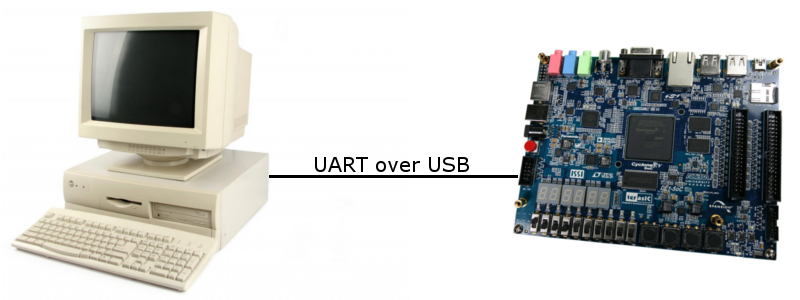
\includegraphics[width=6in]{system-architecture-basic.png}
\caption{Architektura klient-serwer systemu}
\end{figure}

\begin{figure}[!h]
\label{fig:system-architecture}
\centering
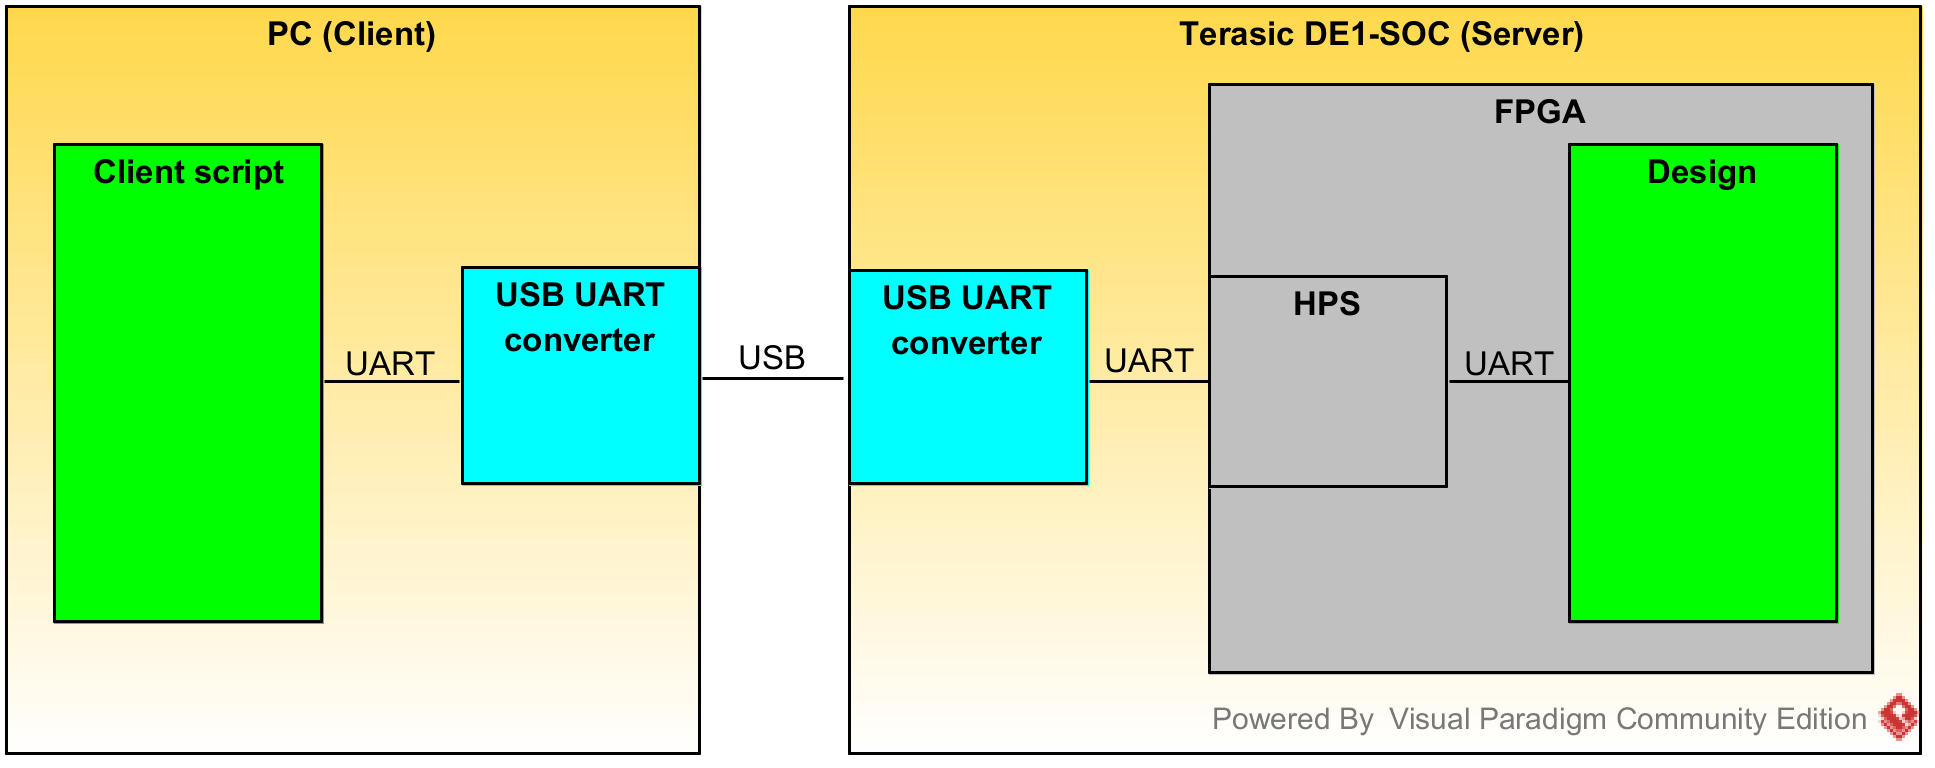
\includegraphics{system-architecture.png}
\caption{Części składowe systemu}
\end{figure}

Serwer (płytka Terasic DE1-SOC) wyposażony jest w układ FPGA, który jest zaprogramowany tak, aby realizował komunikację UART oraz szyfrowanie i deszyfrowanie AES. W układzie FPGA znajdującym się na tej płytce jest zintegrowany procesor ARM (HPS - ang. \textit{hard processor system}), do którego podłączone są sygnały UART biegnące do układu konwertera URAT-USB. Ponieważ te sygnały nie są bezpośrednio podłączone do programowalnej części układu, komunikacja musi zachodzić przez piny HPS, które są skonfigurowane tak, aby FPGA miało do nich dostęp oraz kontrolę (rozdz. \ref{sec:uart-qsys}).

Klientem jest komputer PC z systemem operacyjnym Ubuntu. Programem udostępniającym użytkownikowi funkcjonalność szyfrowania i deszyfrowania plików jest jest skrypt, który odpowiada za komunikację z serwerem wykonującym zlecona zadania.

Komunikacja między klientem a serwerem odbywa się przez kabel USB, którym tunelowany jest sygnał UART. Końcówką tunelu po stronie serwera jest konwerter UART-USB firmy FTDI. Po stronie klienta tunel obsługiwany jest przez wbudowany w system operacyjny sterownik, który umożliwia realizację komunikacji w sposób analogiczny do zwykłego portu szeregowego.


\subsection{Przebieg komunikacji}
\label{sec:przebieg-komunikacji}
Komunikacja między komputerem (klientem) a układem FPGA (serwerem) w celu zaszyfrowania informacji przebiega według schematu:
\begin{enumerate}[noitemsep]
\item Klient wysyła bajt ENC lub DEC wskazujący, czy dane mają być szyfrowane czy deszyfrowane.
\item Serwer odpowiada bajtem ACK jeśli odebrał bajt o wartości ENC lub DEC, NACK w innym przypadku.
\item Jeśli klient otrzymał NACK kończy działanie.
\item Klient wysyła blok zawierający 128 młodszych bajtów klucza oraz 2 bajty CRC16.
\item Serwer odpowiada ACK jeśli blok został przesłany poprawnie(suma kontrolna CRC16 się zgadza), NACK w przeciwnym przypadku.
\item Jeśli klient otrzymał NACK, retransmituje blok oraz oczekuje na potwierdzenie. Retransmisja wykonywana jest do skutku.
\item Klient wysyła blok zawierający 128 starszych bajtów klucza oraz 2 bajty CRC16.
\item Serwer odpowiada ACK jeśli blok został przesłany poprawnie, NACK w przeciwnym przypadku.
\item Jeśli klient otrzymał NACK, retransmituje blok oraz oczekuje na potwierdzenie. Retransmisja wykonywana jest do skutku.
\item Klient wysyła blok zawierający wektor inicjalizacji oraz 2 bajty CRC16.
\item Serwer odpowiada ACK jeśli blok został przesłany poprawnie, NACK w przeciwnym przypadku.
\item Jeśli klient otrzymał NACK, retransmituje blok oraz oczekuje na potwierdzenie. Retransmisja wykonywana jest do skutku.
\item Klient wysyła pierwszy blok danych oraz 2 bajty CRC16.
\item Serwer odpowiada ACK jeśli blok został przesłany poprawnie, NACK w przeciwnym przypadku.
\item Jeśli klient otrzymał NACK, retransmituje blok oraz oczekuje na potwierdzenie. Retransmisja wykonywana jest do skutku.
\item Serwer szyfruje otrzymany blok, wysyła go oraz 2 bajty CRC16. Jednocześnie Klient wysyła kolejny blok do zaszyfrowania.
\item Serwer sprawdza CRC16 i wysyła bajt ACK jeśli blok został otrzymany poprawnie lub NACK w przeciwnym przypadku. Jednocześnie klient postępuje analogicznie.
\item Jeśli odebrany przez serwer blok jest poprawny, oraz jeśli otrzymał od klienta bajt ACK, szyfruje otrzymany blok oraz odsyła go do klienta. W przeciwnym przypadku retransmituje poprzedni zaszyfrowany blok.
\item Jeśli odebrany przez klienta blok jest poprawny, oraz jeśli otrzymał od serwera bajt ACK, wysyła kolejny blok do zaszyfrowania. W przeciwnym wypadku retransmituje poprzedni blok.
\item Wymiana bloków zachodzi dopóki wszystkie informacje nie zostaną zaszyfrowane. O końcu transmisji decyduje klient. Po wysłaniu ostatniego bloku i odebraniu przedostatniego zaszyfrowanego bloku, jeśli zaszyfrowany blok zastał odebrany poprawnie, zamiast ACK wysyła FIN.
\item Serwer po odebraniu bajtu FIN szyfruje ostatni blok oraz odsyła go do klienta.
\item Jeśli klient otrzymał ostatni blok poprawnie wysyła bajt ACK oraz kończy działanie, w przeciwnym wypadku wysyła NACK.
\item Jeśli serwer otrzymał bajt ACK przechodzi do stanu oczekiwania na rozpoczęcie kolejnego procesu szyfrowania. W przeciwnym wypadku retransmituje ostatni zaszyfrowany blok oraz czeka na potwierdzenie. Retransmisja wykonywana jest do skutku.
\end{enumerate}

\begin{figure}[!h]
\centering
\begin{tikztimingtable}[timing/wscale=2.9]
  \textit{RX} & h d{ENC} h      1.5D{KEY\_LOW} h      1.5D{KEY\_HIGH} h      1.5D{INIT\_V} h      1.5D{D1\_PLAIN} h      1.5D{D2\_PLAIN}  d{FIN} 1.5H             d{ACK} h\\
  \textit{TX} & h h      d{ACK} 1.5H           d{ACK} 1.5H            d{ACK} 1.5H          d{ACK} 1.5H            d{ACK} 1.5D{D1\_CYPHER} d{ACK} 1.5D{D2\_CYPHER} h      h\\
\extracode
\tablerules
\end{tikztimingtable}
\label{fig:communication-example}
\caption{Przebieg komunikacji w celu zaszyfrowania dwóch bloków}
\end{figure}

\begin{figure}
\centering
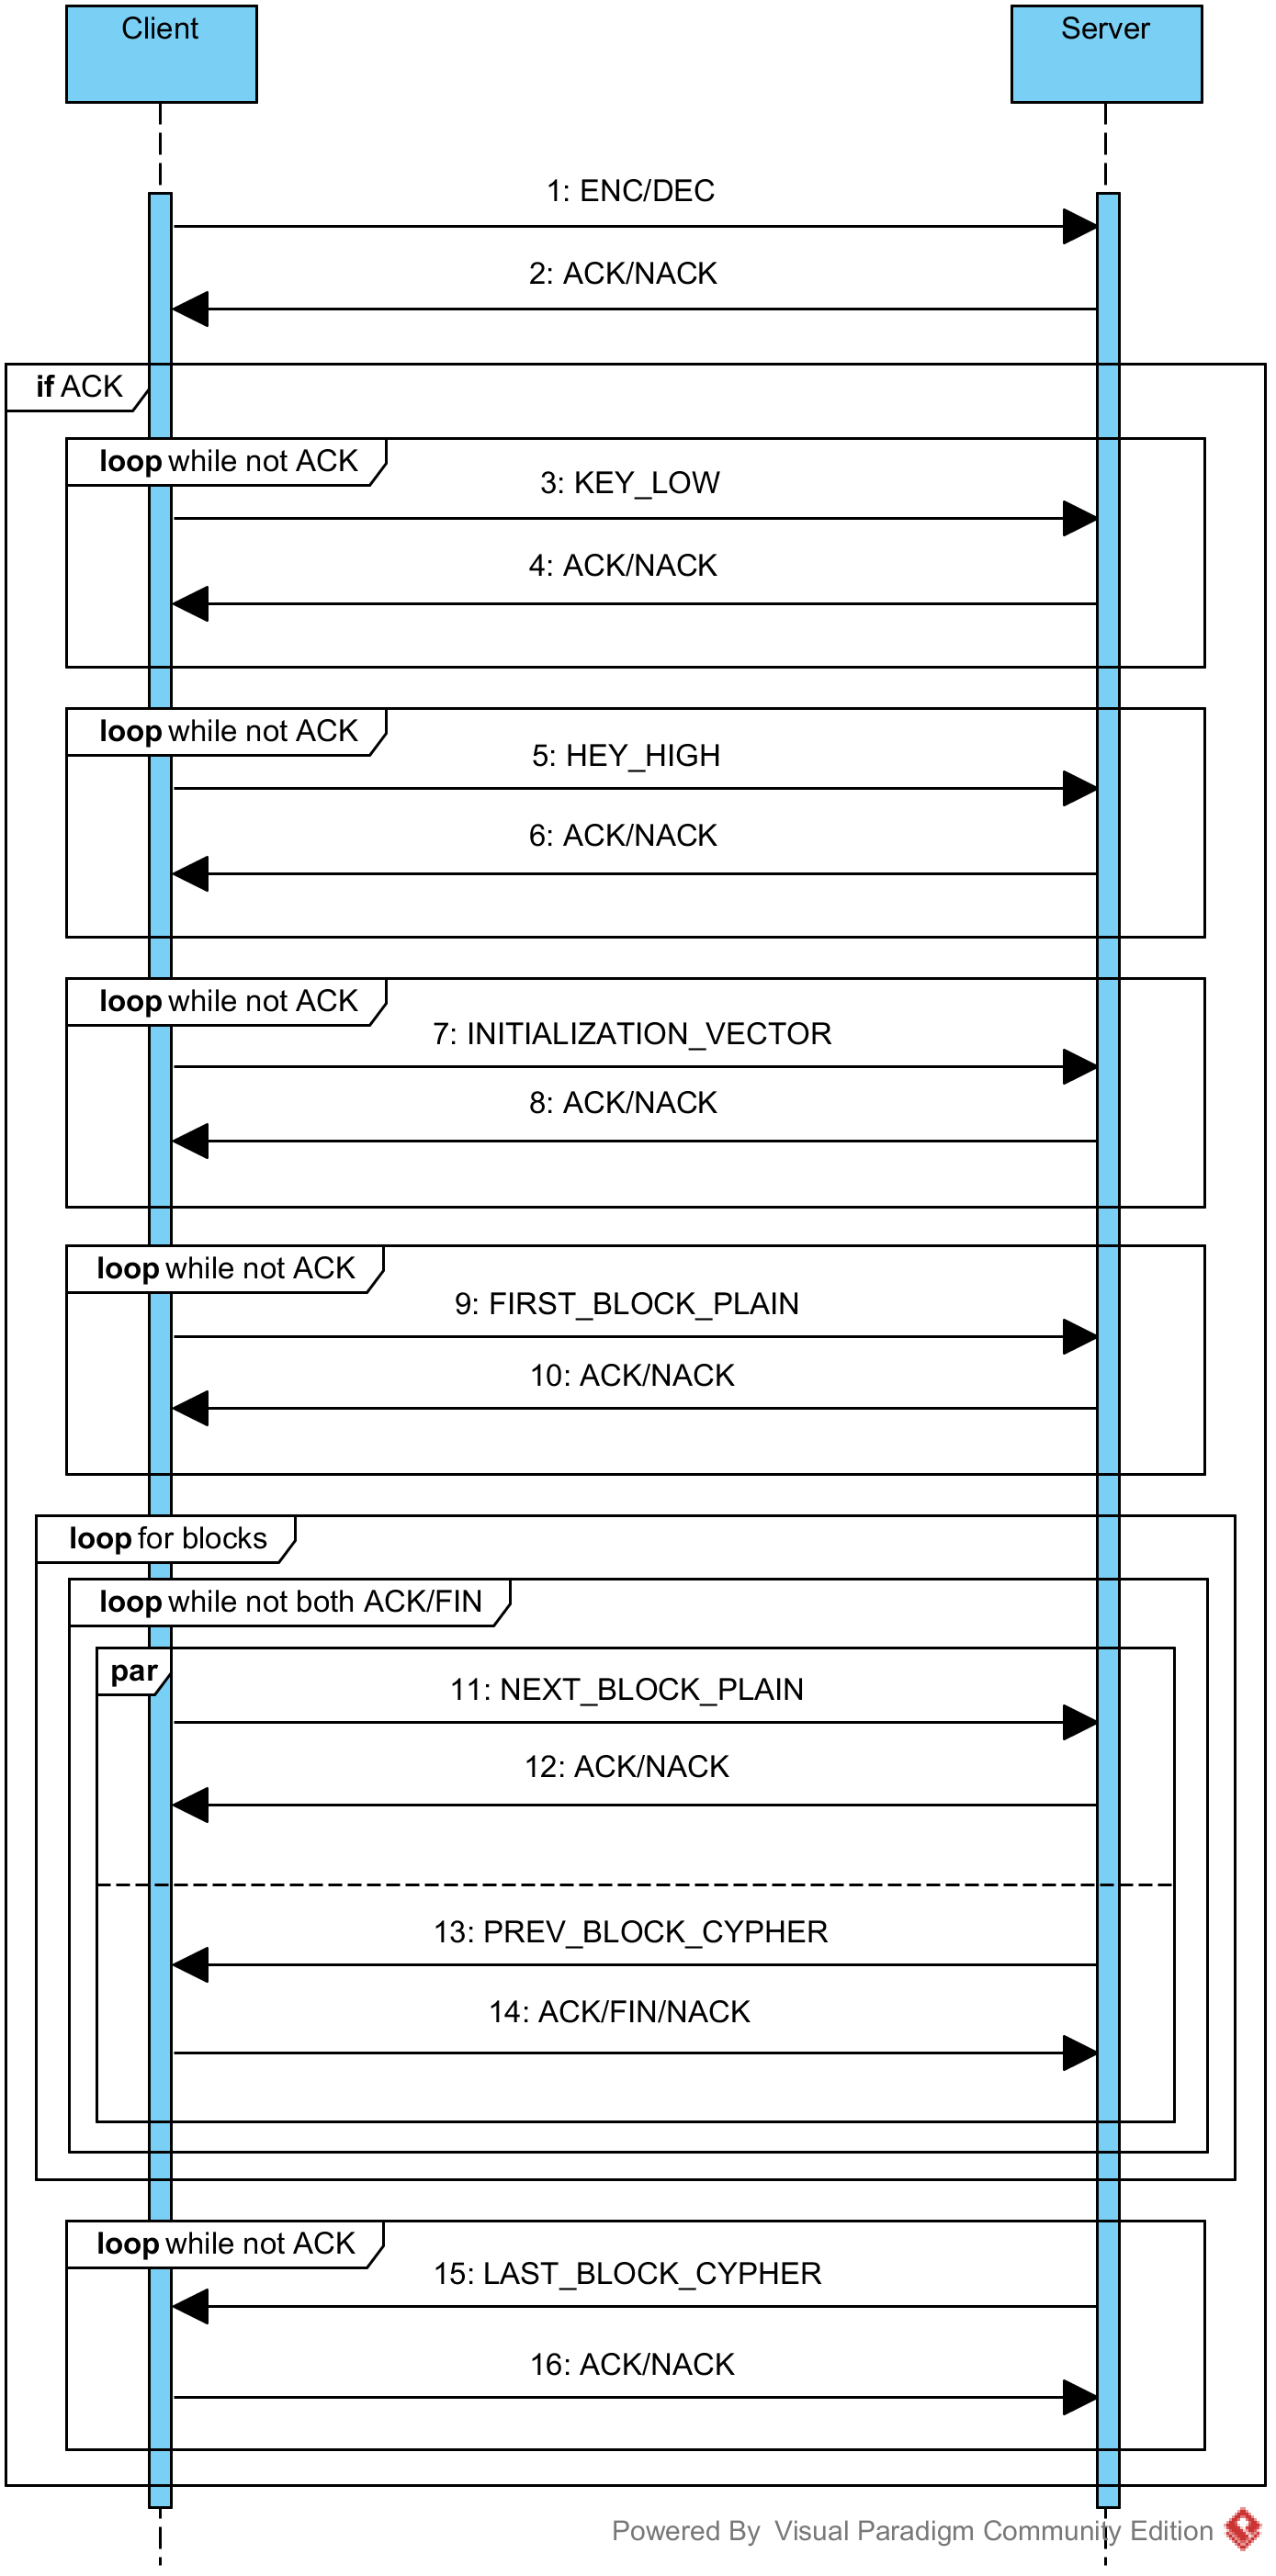
\includegraphics{communication-sequence.png}
\label{fig:communication-sequence}
\caption{Diagram sekwencji komunikacji między klientem a serwerem}
\end{figure}

Schemat \ref{fig:communication-sequence} przestawia diagram sekwencji komunikacji między klientem a użytkownikiem, a rysunek \ref{fig:communication-example} demonstruje przebieg komunikacji w celu zaszyfrowania dwóch bloków danych.

\newpage
\subsection{Struktura projektu FPGA}
Projekt, którym posłuży do zaprogramowania układu FPGA serwera podzielony jest na moduły (rys. \ref{fig:modules}):
\begin{description}
\item[\textit{communicator}] -- moduł odpowiedzialny za zarządzanie procesem przesyłania danych oraz szyfrowania lub deszyfrowania. Główną częścią modułu jest maszyna maszyna stanów (\textit{FSM}), która struje pozostałymi modułami.
\item[\textit{aes\_encryption}] -- moduł szyfrujący bloki AES.
\item[\textit{aes\_decryption}] -- moduł deszyfrujący bloki AES.
\item[\textit{uart\_rx}] -- moduł odbierający bajty.
\item[\textit{uart\_tx}] -- moduł wysyłający bajty.
\item[\textit{block\_serializer}] -- moduł formujący bloki AES ze strumienia odebranych bajtów.
\item[\textit{block\_deserializer}] -- moduł transformujący bloki AES w strumień bajtów do wysłania.
\item[\textit{MUX ENC/DEC}] -- selektor używany do przełączania trybu działania układu (szyfrowane / deszyfrowanie).
\item[\textit{MUX BLOCK/ACK}] -- selektor używany do przełączania źródła wysyłanych bajtów -- z modułu \textit{block\_serializer} (BLOCK) lub potwierdzeń odbioru (ACK).
\item[\textit{HPS}] -- komponent odpowiadający zintegrowanemu procesorowi ARM.
\end{description}

\begin{figure}[!h]
\centering
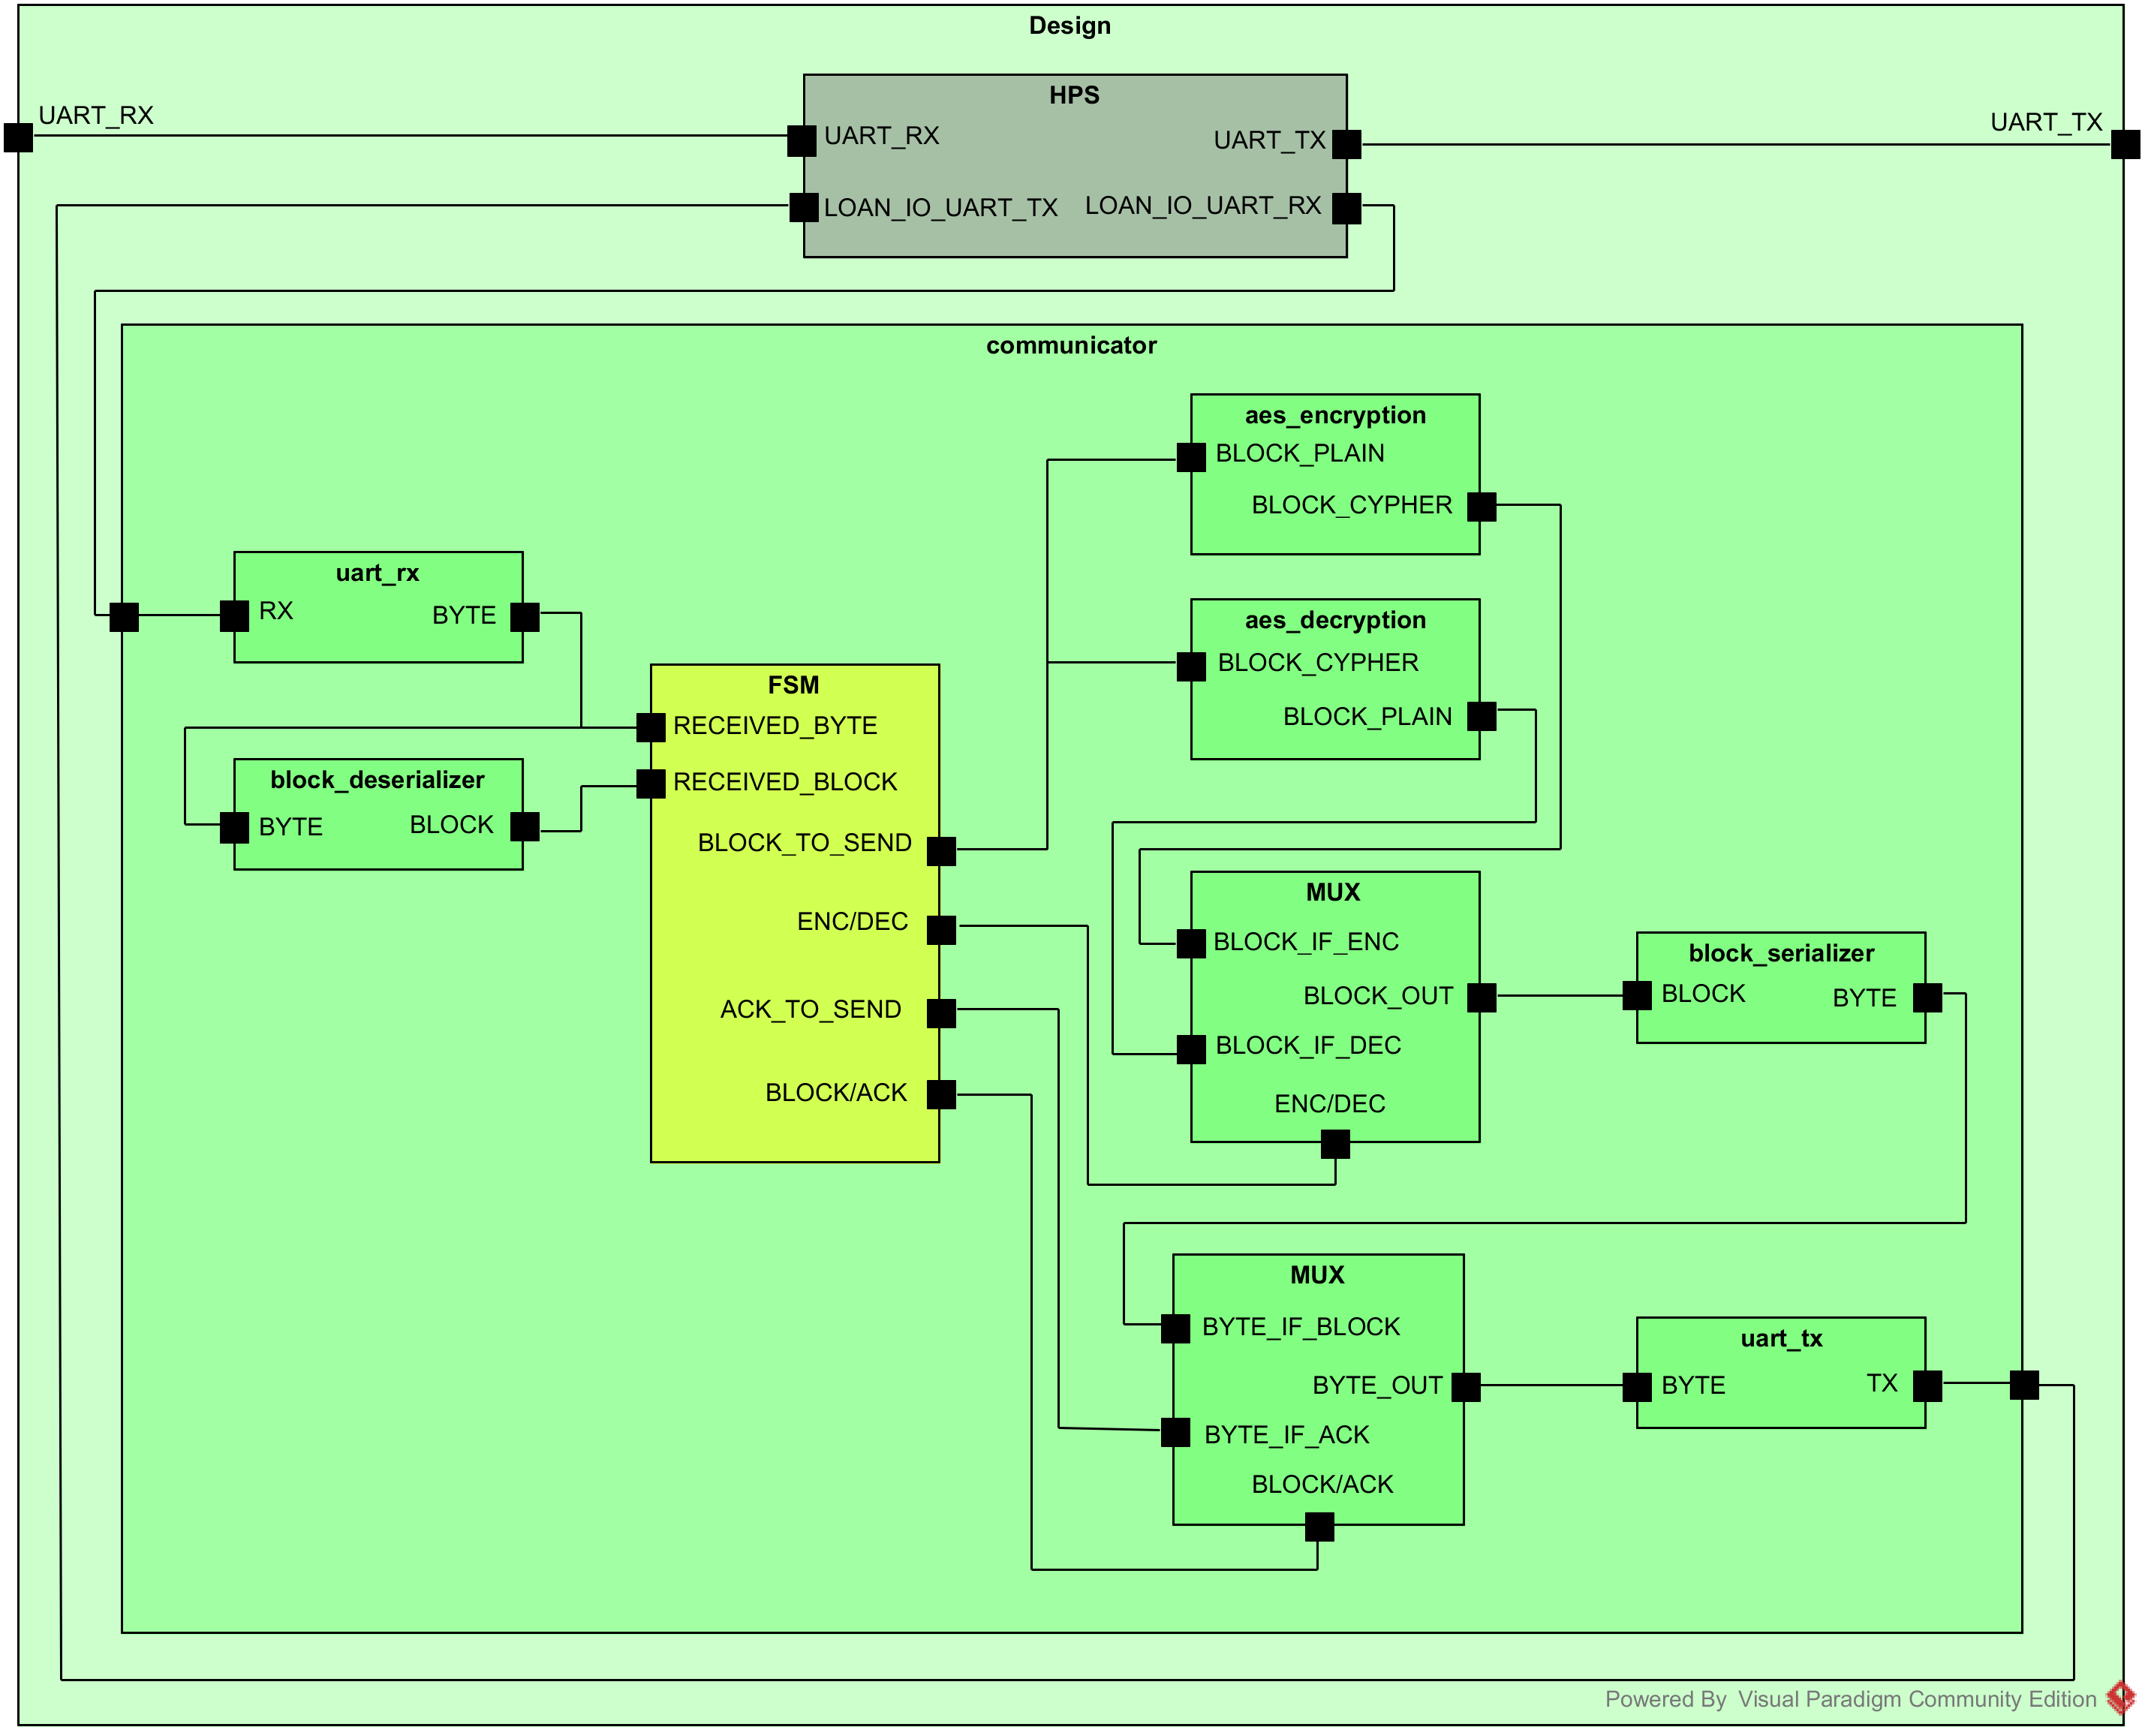
\includegraphics[width=\textwidth]{modules.png}
\label{fig:modules}
\caption{Schemat projektu FPGA}
\end{figure}

Wszystkie moduły wchodzące w skład projektu (rys. \ref{fig:modules}) są szczegółowo opisane w rozdziale \ref{sec:szczegoly-implementacyjne}.
\section{Szczegóły implementacyjne}
\label{sec:szczegoly-implementacyjne}

\subsection{Wykorzystane technologie oraz narzędzia programistyczne}
Projekt jest realizowany na platformie FPGA, więc musi zostać napisany w języku opisu sprzętu. Wykorzystany został język VHDL, ze względu na jego silną kontrolę typów, która pozwala na wczesne wykrywanie niektórych błędów podczas kompilacji, co okazało się bardzo pomocne podczas implementowania modułów AES.

Środowiskiem programistycznym, które zostało wykorzystane do realizacji tego projektu jest Altera Quartus Prime 15.1 Lite Edition. Taki wybór był podyktowany faktem, że wykorzystana w projekcie płytka Terasic DE1-SOC wyposażona jest w układ FPGA firmy Altera, a Quartus jest jedynym środowiskiem przeznaczonym do tworzenia oprogramowania dla układów FPGA tej firmy.

Do realizacji projektu zostało wykorzystane narzędzie QSys, które wchodzi w skład środowiska Quartus oraz służy do integracji zasobów dostępnych na płytce w projekcie, np. HPS, RAM. Pozwala również na konfigurację tych komponentów, co ma kluczowe znaczenie dla wykorzystania znajdującego się na płytce konwertera USB UART (patrz rozdział \ref{sec:uart-qsys}).

Do przygotowania karty SD wykorzystane zostało środowisko Altera SoC FPGA Embedded Design Suite 15.1, które zawiera narzędzia programistyczne przeznaczone do tworzenia projektów korzystających zarówno z programowalnej części FPGA jak i procesora HPS. Użyte zostało narzędzie \textit{bsp-editor}, które posłużyło do wygenerowania preloadera (patrz rozdział \ref{sec:uart-preloader-gen}).

Testy implementowanych komponentów były realizowane jako symulacje funkcyjne przy pomocy narzędzi wchodzących w skład środowiska programistycznego Quartus.


\subsection{Przygotowanie oraz konfiguracja projektu}
\label{sec:przygotowanie-projektu}

Terasic -- producent wykorzystanej w tym projekcie płytki płytki DE1-SOC -- opracował i udostępnił na płycie CD dołączonej do zestawu \cite{??} projekt bazowy GHRD (ang. \textit{Golden Hardware Reference Design}). Jest to projekt skonfigurowany do poprawnego działania z płytką DE1-SOC, w którym ustawione są m.in.
\begin{itemize}[noitemsep]
\item model układu FPGA znajdującego się na płytce
\item konfiguracja pinów
\item podstawowe ograniczenia czasowe układu
\item projekt QSys reprezentujący zintegrowany procesor HPS (ang. \textit{Hard Processor System})
\item główny plik projektu (ang. \textit{top-level entity}) wraz z dodanym komponentem reprezentującym HPS
\end{itemize}
Projekt GHRG zawiera podstawowe ustawienia, więc umożliwia programiście skrócenie etapu konfiguracji projektu oraz szybkie rozpoczęcie pracy nad projektowanym układem. Bazą dla tego projektu był GHRD.

Do konwersji sygnału USB do UART wykorzystany został znajdujący się na płytce Terasic DE1-SOC układ firmy FTDI. Jego sygnały nie są jednak podłączone bezpośrednio do programowalnej części układu FPGA, lecz do zintegrowanego procesora ARM. Aby uzyskać dostęp do jego sygnałów z FPGA należy odpowiednio dostosować projekt oraz stworzyć i wgrać na kartę SD preloader, który podczas uruchamiania płytki przestawi piny UART w odpowiedni tryb działania oraz określi ich kierunek.

\subsubsection{Konfiguracja pinów UART}
\label{sec:uart-qsys}
Aby skonfigurować projekt tak, aby układ FPGA miał dostęp do sygnałów UART konwertera USB UART podłączonych do HPS, należy wykonać następujące czynności \cite{altera-youtube-loanerio, altera-forum-fgga-hps-access, altera-forum-cant-rx}:

\begin{enumerate}
\item Otworzyć w edytorze QSys plik \textit{soc-system.qsys}
\item Wybrać komponent \textit{hps\_0} (rys. \ref{fig:qsys-hps} A) oraz w zakładce \textit{Peripheral Pins} (rys. \ref{fig:qsys-hps} B) dokonać zmian:
	\begin{itemize}[noitemsep,nolistsep]
	\item Zmienić wartość \textit{UART0 pin} na \textit{FPGA} (rys. \ref{fig:qsys-hps} C)
	\item Zmienić wartość \textit{UART0 mode} na \textit{Full} (rys. \ref{fig:qsys-hps} C)
	\item Zaznaczyć \textit{LOANIO 49} oraz \textit{LOANIO 50} (rys. \ref{fig:qsys-hps} D)
	\end{itemize}
\item Opcjonalnie można oczyścić projekt z komponentów, które zostały skonfigurowane w GHRD a nie zostaną wykorzystane: \textit{dipsw\_pio}, \textit{button\_pio}, \textit{led\_pio}.
\item Zapisać zmiany, wygenerować kod VHDL klikając przycisk \textit{Generate HDL...} (rys. \ref{fig:qsys-hps} E) oraz opuścić edytor (rys. \ref{fig:qsys-hps} F).
\item W głównym pliku projektu (ang. \textit{Top-Level Entity}) zmodyfikować komponent \textit{soc-system} tak, aby był zgodny z jego na nowo wygenerowaną wersją.
\item Przypisać wartość \textit{'1'} sygnałom:
	\begin{itemize}[noitemsep,nolistsep]
	\item \textit{hps\_0\_uart0\_cts}
	\item \textit{hps\_0\_uart0\_dsr}
	\item \textit{hps\_0\_uart0\_dcd}
	\item \textit{hps\_0\_uart0\_ri}
	\item \textit{hps\_0\_uart0\_rxd}
	\end{itemize}
\item Sygnał \textit{hps\_0\_hps\_io\_hps\_io\_gpio\_inst\_LOANIO49} przypisać do pinu \textit{HPS\_UART\_RX}.
\item Sygnał \textit{hps\_0\_hps\_io\_hps\_io\_gpio\_inst\_LOANIO50} przypisać do pinu \textit{HPS\_UART\_TX}.
\item Wektor sygnałów \textit{hps\_0\_h2f\_loan\_io\_oe} określa kierunek pinów pinów \textit{LOANIO}.
	\begin{itemize}[noitemsep,nolistsep]
	\item Do sygnału \textit{hps\_0\_h2f\_loan\_io\_oe(49)}, który odpowiada sygnałowi UART RX przypisać wartość \textit{'1'}, co odpowiada kierunkowi \textit{out}.
	\item Do sygnału \textit{hps\_0\_h2f\_loan\_io\_oe(50)}, który odpowiada sygnałowi UART TX przypisać wartość \textit{'0'}, co odpowiada kierunkowi \textit{in}.
	\end{itemize}
\end{enumerate}

\begin{figure}[!h]
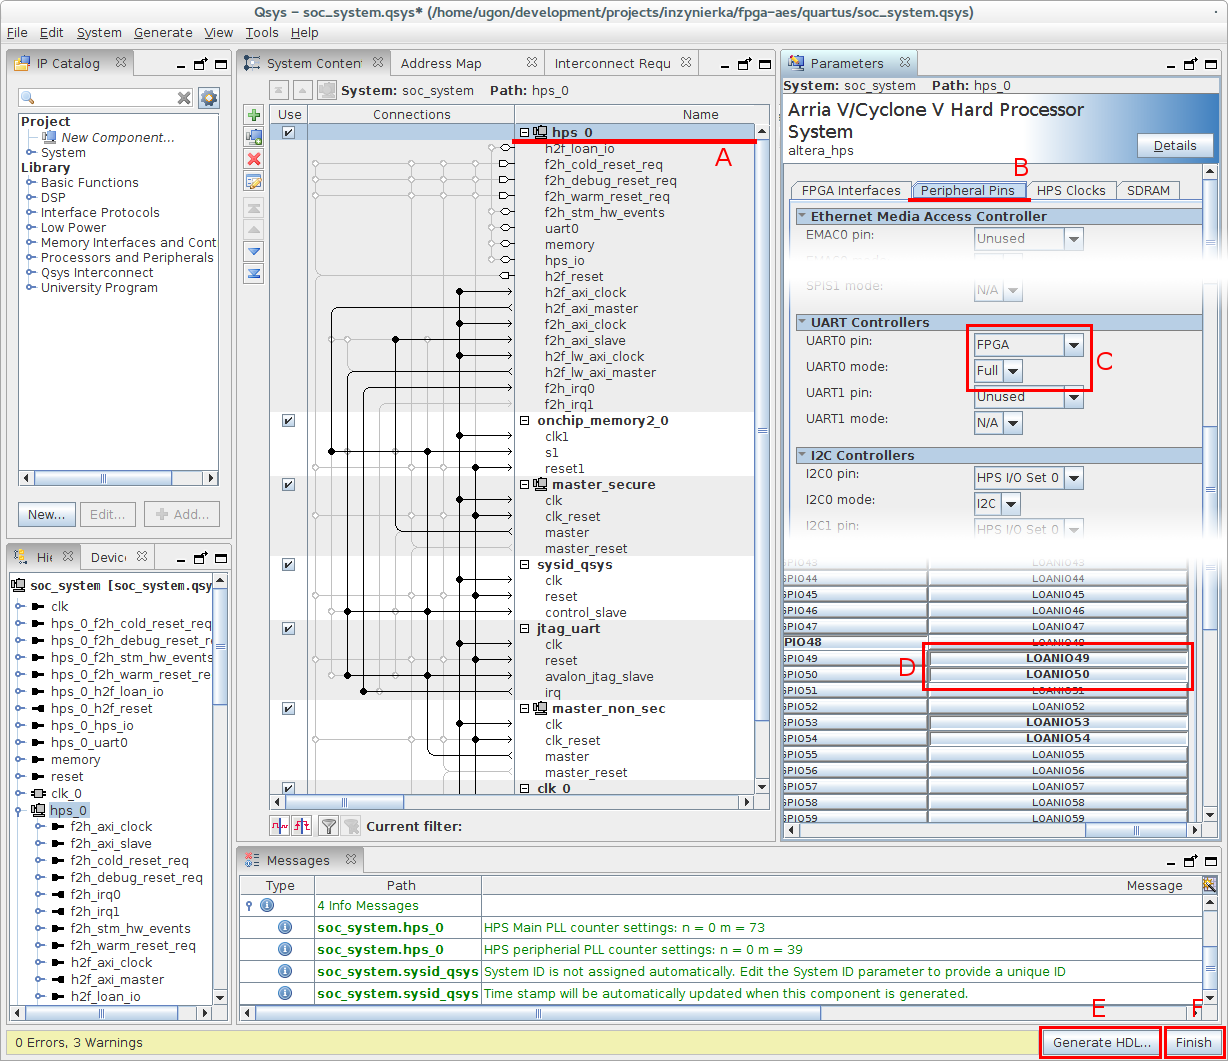
\includegraphics[width=\textwidth]{qsys.png}
\caption{Konfiguracja komponentu HPS w edytorze QSys}
\label{fig:qsys-hps}
\end{figure}

Wykonane zmiany spowodują, że:
\begin{itemize}[noitemsep]
\item Sygnał \textit{hps\_0\_h2f\_loan\_io\_out(49)} będzie odpowiadał sygnałowi UART RX oraz będzie poprawnie połączony z konwerterem USB-UART firmy FTDI.
\item Sygnał \textit{hps\_0\_h2f\_loan\_io\_out(50)} będzie odpowiadał sygnałowi UART TX oraz będzie poprawnie połączony z konwerterem USB-UART firmy FTDI
\end{itemize}


\subsubsection{Przygotowanie preloadera}
\label{sec:uart-preloader-gen}
Aby przy starcie płytki piny UART zostały poprawnie połączone z układem FPGA należy z plików powstałych w wyniku kompilacji projektu wygenerować preloader. Aby to zrobić posłużyłem się narzędziem \textit{bsp-editor} będącym częścią oprogramowania Quartus, zgodnie z instrukcją znalezioną w internecie \cite{rocketboards-preloader}.

\subsubsection{Skrypt startowy programujący układ FPGA}
Aby automatycznie zaprogramować układ FPGA podczas startu urządzenia stworzyłem skrypt, który będzie się wykonywał w fazie U-Boot \cite{rocketboards-uboot-script}.
\begin{lstlisting}
fatload mmc 0:1 $fpgadata soc_system.rbf;
fpga load 0 $fpgadata $filesize;
\end{lstlisting}
Do programowania układu FPGA przy pomocy skryptu potrzebny jest plik konfiguracyjny w formacie \textit{.rbf}. Można go stworzyć konwertując przy pomocy środowiska Quartus plik \textit{.sof} powstały w wyniku kompilacji projektu \cite{rocketboards-sof-to-rfb}. Użyłem trybu programowania \textit{Fast Passive Parallel X16}, któremu odpowiada ustawienie przełączników MSEL[0:4] znajdujących się na płytce na wartość 00100.

\subsubsection{Przygotowanie karty SD}
Najłatwiejszym sposobem na stworzenie karty SD zawierającej potrzebne pliki jest modyfikacja dostarczonych na płycie CD do płytki Terasic DE1-SOC przykładowych obrazów. Lista kroków realizujących to zadanie przy użyciu komputera z systemem operacyjnym Linux \cite{rocketboards-booting-prebuild, rocketboards-updating-sd}:
\begin{enumerate}
\item Po włożeniu karty SD do czytnika należy określić jej ścieżkę w systemie operacyjnym, najlepiej analizując plik \textit{/proc/partitions}. Załóżmy, że ścieżką karty jest \textit{/dev/sdx}.
\begin{lstlisting}
  $ cat /proc/partitions
\end{lstlisting}

\item Wgrać dostarczony przez producenta obraz \textit{DE1\_SoC\_SD.img} na kartę SD.
\begin{lstlisting}
  $ sudo dd if=DE1\_SoC\_SD.img of=/dev/sdx bs=1M
  $ sudo sync
\end{lstlisting}

\item Zastąpić domyślny preloader
\begin{lstlisting}
  $ sudo dd if=preloader-mkpimage.bin of=/dev/sde3 bs=64k seek=0
  $ sudo sync
\end{lstlisting}

\item Wgrać skrypt U-Boot oraz plik zawierający konfigurację układu FPGA na partycję FAT \textit{/dev/sdx1} dowolnym sposobem (np. korzystając z systemowego eksploratora plików).
\end{enumerate}

Aby przy starcie płytki programowanie FPGA przebiegło pomyślnie, należy umieścić kartę SD w czytniku oraz ustawić przełączniki MSEL[4:0] w pozycji 00100.

\subsubsection{Główny zegar}
\label{clk-16}
Główny zegar \textit{CLK\_16}, którym taktowany będzie projektowany układ ma częstotliwość
\begin{equation}
f_{CLK\_16} = 16 * UART\_BAUD\_RATE
\end{equation}
gdzie \textit{UART\_BAUD\_RATE} jest szybkością transmisji sygnału UART wyrażoną w baudach, która dla tego projektu wynosi 115200 baudów. Taka wartość podyktowana jest faktem, że częstą praktyką interpretacji sygnału UART, jest jego próbkowanie z częstotliwością 16 razy szybszą niż częstotliwość zmian sygnału.

Częstotliwość zegara \textit{CLK\_16} jest o wiele niższa niż dostępny w układzie FPGA zegar o częstotliwości 50MHz. Pozwoliło to na uzyskanie żądanej częstotliwości przy pomocy prostego dzielnika częstotliwości.

\begin{figure}[!h]
\begin{lstlisting}[style=vhdl, caption={Dzielnik częstotliwości \textit{uart\_prescaler}}, captionpos=b]
entity uart_prescaler is
	port (
		clk_in  : in  std_logic;  --50MHz
		clk_out : out std_logic); --16 * 115200Hz
end uart_prescaler;

architecture uart_prescaler_impl of uart_prescaler is
	signal clk : std_logic := '0';
begin
	clk_out <= clk;
	
	process (clk_in) 
		variable counter : Integer range 0 to 13 := 0;
	begin	
		if(rising_edge(clk_in)) then
			case counter is
				when 13 =>
					clk <= not clk;
					counter := 0;
				when others =>
					counter := counter + 1;
			end case;
		end if;
	end process;
end uart_prescaler_impl;
\end{lstlisting}
\end{figure}

Układ jest wyzwalany rosnącymi zboczami zegara \textit{CLK\_16}. Jeśli akcja mająca miejsce w danym rosnącym zboczu zależy od wartości innego sygnału, to ma on stałą wartość co najmniej od poprzedzającego do następnego zbocza malejącego.

\subsubsection{Synchronizacja sygnału UART RX}
\label{uart-sync}
Sygnał UART RX pochodzi z peryferyjnego konwertera USB-UART firmy FTDI, który jest w domenie innego zegara. Powoduje to, że w momencie wystąpienia zbocz rosnących lub malejących głównego zegara, sygnał RX może nie mieć dobrze określonej wartości (np. również być w trakcie zbocza). Może to prowadzić do wystąpienia stanów metastabilnych \cite{altera-metastability} i w efekcie doprowadzić do niedeterministycznego działania układu. Aby temu zapobiec sygnał RX został zsynchronizowany przy pomocy dwóch przerzutników typu D wyzwalanych głównym zegarem \cite{altera-metastability, 2ff-synchronization}. 

\begin{figure}[!h]
\centering
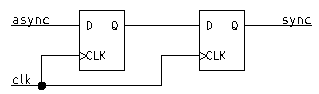
\includegraphics[width=100mm,scale=1.5]{2ff.pdf}
\caption{Synchronizacja sygnału przy użyciu dwóch przerzutników typu D}
\end{figure}

Jest to standardowa technika, która powoduje drastyczne zmniejszenie prawdopodobieństwa wystąpienia stanów metastabilnych z powodu używania sygnałów pochodzących z domen innych zegarów.

\subsubsection{Ograniczenia czasowe}
Aby mieć gwarancję, że projekt nie będzie zachowywał się niedeterministyczne ze względu na złe ułożenie ścieżek sygnałów w chipie FPGA powodujące zbyt długi czas propagacji, zdefiniowane zostały odpowiednie ograniczenia czasowe. Do tego celu posłużyła konsola w narzędziu TimeQuest Timing Analyzer będącym częścią środowiska programistycznego Quartus. Zdefiniowane ograniczenia to:

\begin{itemize}
\item Zewnętrzny zegar \textit{CLK\_50} o częstotliwości 50MHz
\begin{lstlisting}[basicstyle=\footnotesize]
create_clock -name {CLK_50} -period 20.000 { CLOCK_50 }
\end{lstlisting}

\item Główny zegar projektu \textit{CLK\_16}
\begin{lstlisting}[basicstyle=\footnotesize]
create_generated_clock -name {CLK_16} -source {CLOCK_50} 
	-divide_by 26 { uart_prescaler0|clk|q }
\end{lstlisting}

\item Sygnał w module \textit{block\_serializer} (rozdz. \ref{??}), na którego zbocze rosnące musiał być wrażliwy proces sterujący sygnałem zakończenia wysyłania bloku -- \outsignal{FINISHED\_TRANSMITTING}.
\begin{lstlisting}[basicstyle=\footnotesize]
create_generated_clock -name {SERIALIZER_CLK} 
	-source {uart_prescaler0|clk|q} -divide_by 2 -offset 260.000 
	{ communicator0|block_serializer0|forward_start|q }
\end{lstlisting}

\item Sygnał w module \textit{block\_deserializer} (rozdz. \ref{??}), na którego zbocze rosnące musiał być wrażliwy proces sterujący sygnałami odebranego bloku \outsignal{AES\_BLOCK[127:0]} oraz zakończenia odbierania \outsignal{FINISHED\_LISTENING}.
\begin{lstlisting}[basicstyle=\footnotesize]
create_generated_clock -name {DESERIALIZER_CLK} \
	-source {uart_prescaler0|clk|q} -divide_by 2 -offset 260.000 
	{ communicator0|block_deserializer0|forward_finished|q }
\end{lstlisting}

\end{itemize}

Są to wszystkie sygnały pełniące w tym projekcie rolę zegarów.

\subsubsection{Moduł odbierający bajty UART}
Interfejs układu odbierającego bajty UART \textit{uart\_rx}:

\begin{interface}{FINISHED\_LISTENING}
	\item[\insignal{CLK\_16}] główny zegar układu.
	\item[\insignal{RX}] zsynchronizowany przy pomocy dwóch przerzutników typu D sygnał UART RX, wychodzący z konwertera USB-UART.
	\item[\insignal{START\_LISTENING}] sygnał wprowadzający komponent w stan oczekiwania na bajt.
	\item[\outsignal{BYTE[7:0]}] odebrany bajt. Stabilność sygnału jest gwarantowana, gdy \outsignal{FINISHED\_LISTENING} jest w stanie wysokim.
	\item[\outsignal{FINISHED\_LISTENING}] sygnał informujący o zakończeniu odbierania bajtu oraz gotowość na otrzymanie kolejnego sygnału \insignal{START\_LISTENING} podczas kolejnego zbocza rosnącego zegara \insignal{CLK\_16}.
\end{interface}

Po otrzymaniu sygnału \insignal{START\_LISTENING} moduł rozpoczyna nasłuchiwanie na transmisję. Każdy bit jest próbkowany 16 razy. Wartość bitu jest ustalana na podstawie \textit{głosowania} -- bit jest uznawany za {'1'} jeśli co najmniej dwie z trzech środkowych próbek mają wartość {'1'}, analogicznie dla {'0'}. Transmisja bajtu zostaje uznana za rozpoczętą, jeśli zostanie odebrany bit startu -- gdy zostanie napotkana pierwsza próbka o wartości {'0'} i potwierdzona przez głosowanie. Bajt zostaje uznany za poprawnie odebrany, jeśli zostanie odebrany poprawny bit stopu. Bit stopu jest próbkowany jedynie 9 razy. Jest to minimalna liczba próbek pozwalająca przeprowadzić \textit{głosowanie}. Próbkowanie bitu stopu jest skrócone, ze względu na fakt, że pomimo ustawienia zgodnych parametrów transmisji nadajnika i odbiornika, zegar urządzenia nadającego może być minimalnie szybszy. Prowadzi to do zbyt wolnego odbierania napływających informacji i po kilku odebranych bajtach prowadzi do błędów, co zostało zaobserwowane w trakcie testów. Skrócenie czasu odbierania bitu stopu zapobiega takim sytuacjom.

\begin{figure}[!h]
	\centering
	\begin{tikztimingtable}
	\insignal{CLK\_16}          & 32{cc}  \\
	\insignal{RX}               & HHH    16J{Start}    13D{Data[0]}\\
	\insignal{START\_LISTENING} & LH30L\\
	\extracode
	\tablerules
	\draw[red, ->] (3.5,0) -- (3.5,1);
	\draw[red, ->] (9.5,0) -- (9.5,1);
	\draw[red, ->] (10.5,0) -- (10.5,1);
	\draw[red, ->] (11.5,0) -- (11.5,1);
	\draw[red, ->] (26.5,0) -- (26.5,1);
	\draw[red, ->] (27.5,0) -- (27.5,1);
	\draw[red, ->] (28.5,0) -- (28.5,1);
	\end{tikztimingtable}
\caption{\textit{uart\_rx} -- odbiór bitu startu}
\end{figure}

\begin{figure}[!h]
	\centering
	\begin{tikztimingtable}
	\insignal{CLK\_16}              & 31{cc}  \\
	\insignal{RX}                   & 13D{Data[7]} 16J{Stop} HH   \\
	\outsignal{BYTE[7:0]}           & 22U D 8U \\
	\outsignal{FINISHED\_LISTENING} & 22L H 8L \\
	\extracode
	\tablerules
	\draw[red, ->] (4.5,0) -- (4.5,1);
	\draw[red, ->] (5.5,0) -- (5.5,1);
	\draw[red, ->] (3.5,0) -- (3.5,1);
	\draw[red, ->] (19.5,0) -- (19.5,1);
	\draw[red, ->] (20.5,0) -- (20.5,1);
	\draw[red, ->] (21.5,0) -- (21.5,1);
	\end{tikztimingtable}
\caption{\textit{uart\_rx} -- odbiór bitu stopu}
\end{figure}

\begin{figure}[!h]
	\centering
	\begin{tikztimingtable}[timing/wscale=2.8]
  	\insignal{CLK\_UART}            & c cc        cc         cc         cc         cc         cc         cc         cc         cc         cc       c \\
  	\insignal{RX}                   & u J{Start}  D{Data[0]} D{Data[1]} D{Data[2]} D{Data[3]} D{Data[4]} D{Data[5]} D{Data[6]} D{Data[7]} K{Stop}  u \\
  	\outsignal{BYTE[7:0]}           & 10U 0.5d 1.5u \\
	\outsignal{FINISHED\_LISTENING} & 10L 0.5h 1.5l \\
	\extracode
	\tablerules
	\end{tikztimingtable}
\caption{\textit{uart\_rx} -- odbiór całej ramki UART}
\end{figure}
\newpage
\subsection{Moduł wysyłający bajty UART}
Moduł \textit{uart\_tx} wysyła bajty do klienta przez interfejs UART.

\begin{figure}[!h]
\begin{lstlisting}[style=vhdl, captionpos=b, caption={\textit{uart\_tx} -- interfejs modułu}]
port (
	reset_n               : in  std_logic;
	clk_16                : in  std_logic;
	tx                    : out std_logic;

	byte                  : in  std_logic_vector(byte_bits - 1 downto 0);
	start_transmitting    : in  std_logic;
	finished_transmitting : out std_logic);
\end{lstlisting}
\end{figure}

Opis sygnałów interfejsu modułu \textit{uart\_tx}:
\begin{interface}{FINISHED\_TRANSMITTING}
\item[\insignal{CLK\_16}] główny zegar układu.
\item[\insignal{START\_TRANSMITTING}] sygnał rozpoczynający wysyłanie danych.
\item[\insignal{BYTE[7:0]}] bajt do wysłania. Stabilność sygnału jest wymagana, gdy \insignal{START\_TRANSMITTING} jest w stanie wysokim.
\item[\outsignal{TX}] sygnał UART TX wychodzący do konwertera USB-UART.
\item[\outsignal{FINISHED\_TRANSMITTING}] sygnał sygnalizujący zakończenie wysyłania bajtu oraz gotowość na otrzymanie kolejnego sygnału \insignal{START\_TRANSMITTING} podczas kolejnego zbocza rosnącego.
\end{interface}

Moduł rozpoczyna transmisję po otrzymaniu sygnału \insignal{START\_TRANSMITTING} (rys. \ref{fig:uart-tx-stop-start}). Wysyłany jest bajt (rys. \ref{fig:uart-tx-frame}) dostarczony do modułu przez sygnał \insignal{BYTE[7:0]}. Bity startu, danych oraz stopu są wysyłane przez 16 cykli zegara \insignal{CLK\_16}. Zakończenie wysyłania ramki UART sygnalizowane jest przez sygnał \outsignal{FINISHED\_TRANSMITTING}, który również oznacza gotowość modułu na rozpoczęcie transmisji kolejnego bitu podczas następnego zbocza rosnącego. Sygnał \outsignal{FINISHED\_TRANSMITTING} wysyłany jest w przedostatnim cyklu zegarowym wysyłania bitu stopu, aby w ostatnim cyklu mógł nadejść następny sygnał \insignal{START\_TRANSMITTING}. Takie rozwiązanie umożliwia prowadzenie transmisji przez moduł z maksymalną możliwą prędkością -- ani jeden cykl zegara nie jest zmarnowany (rys. \ref{fig:uart-tx-stop-start}).

\newpage

\begin{center}
\centering
\resizebox{\textwidth}{!}{
	\begin{tikztimingtable}[timing/wscale=0.9]
	\insignal{CLK\_16}          & 3{cc}       16{cc}     16{cc}     3{cc}\\
	\insignal{START\_TRANS}     & 3U          15UH       16U        3U     \\
	\insignal{BYTE[7:0]}        & 3U          15UD       16U        3U          \\
	\outsignal{TX}              & 3D{Data[7]} 17.777K{Stop}  17.777J{Start} 3D{Data[0]}\\ %to offset crapy scaling
	\outsignal{FINISHED\_TRANS} & 3U          14UHU      16U        3U\\
	\extracode
	\tablerules
	\end{tikztimingtable}
}
\captionof{figure}{\textit{uart\_tx} -- wysłanie bitu stopu i startu}
\label{fig:uart-tx-stop-start}
\end{center}


\begin{center}
\centering
\resizebox{\textwidth}{!}{
	\begin{tikztimingtable}[timing/wscale=3.0]
	\insignal{CLK\_16}          & c              cc        cc         cc         cc         cc         cc         cc         cc         cc         cc       c \\
	\insignal{START\_TRANS}     & 0.5u0.5h 10.5U     \\
	\insignal{BYTE[7:0]}        & 0.5u0.5d 10.5U      \\
	\outsignal{TX}              & u              J{Start}  D{Data[0]} D{Data[1]} D{Data[2]} D{Data[3]} D{Data[4]} D{Data[5]} D{Data[6]} D{Data[7]} K{Stop}  u \\
	\outsignal{FINISHED\_TRANS} & u              9.5U 0.5h 1.5u\\
	\extracode
	\tablerules
	\end{tikztimingtable}
}
\captionof{figure}{\textit{uart\_tx} -- wysłanie całej ramki UART}
\label{fig:uart-tx-frame}
\end{center}
\subsubsection{Moduł deserializujący bajty UART do bloków AES}
Interfejs modułu deserializującego bajty UART do bloków AES \textit{block\_deserializer}:
\begin{interface}{RX\_FINISHED\_LISTENING}
	\item[\insignal{CLK\_16}] główny zegar układu.

	\item[\insignal{RX\_BYTE[7:0]}] sygnał pochodzący z komponentu \textit{uart\_rx}.
	\item[\outsignal{RX\_START\_LISTENING}] sygnał wychodzący do komponentu \textit{uart\_rx}.
	\item[\insignal{RX\_FINISHED\_LISTENING}] sygnał pochodzący z komponentu \textit{uart\_rx}.

	\item[\insignal{START\_LISTENING}] sygnał wprowadzający komponent w stan oczekiwania na blok.
	\item[\outsignal{BLOCK[127:0]}] odebrany blok AES. Stabilność sygnału jest gwarantowana, gdy \outsignal{FINISHED\_LISTENING} jest w stanie wysokim.
	\item[\outsignal{FINISHED\_LISTENING}] sygnał informujący o zakończeniu odbierania bloku AES oraz gotowość na otrzymanie kolejnego sygnału \insignal{START\_LISTENING} podczas następnego zbocza rosnącego zegara \insignal{CLK\_16}.
	\item[\outsignal{CORRECT}] sygnał określający, czy transmisja bloku AES przebiegła bez błędów. Stabilność sygnału jest gwarantowana, gdy \outsignal{FINISHED\_LISTENING} jest w stanie wysokim.
\end{interface}

Po otrzymaniu sygnału \insignal{START\_LISTENING} moduł rozpoczyna nasłuchiwanie na transmisję. Odbieranie bajtów bloku danych wykonywane jest przez przez moduł \textit{uart\_rx}. Kolejność ułożenia bajtów w bloku \outsignal{BLOCK[127:0]} jest zgodna ze standardem AES. W trakcie odbierania obliczana jest suma kontrolna \textit{CRC16}. Po 128 bajtach bloku danych przesyłane są 2 bajty zawierające oczekiwaną, obliczoną po stronie klienta sumę kontrolną. Jeśli jest ona zgodna z tą obliczaną na bieżąco przez moduł, sygnał \outsignal{CORRECT} przyjmuje wartość {'1'}, w przeciwnym wypadku wartość {'0'}. Po odebraniu 130 bajtów moduł zwraca blok \outsignal{BLOCK[127:0]} wraz z informacją o jego poprawności \outsignal{CORRECT} oraz sygnalizuje gotowość na rozpoczęcie nasłuchiwania na kolejne bloki \outsignal{FINISHED\_LISTENING}.

\begin{figure}[!h]
	\centering
	\begin{tikztimingtable}[timing/wscale=0.95]
	\insignal{CLK\_16}          & 3{cc}  16{cc}           16{cc}         \\
	\outsignal{RX\_START\_LIST} & LH     15LH             15LH           L\\
	\insignal{RX\_BYTE[7:0]}    & L      15LD{BLOCK[0]}   15LD{BLOCK[1]} 2L\\
	\insignal{RX\_FIN\_LIST}    & L      15LH             15LH           2L\\
	\insignal{START\_LIST}      & LH     16L              16L            L\\
	\extracode
	\tablerules
	\end{tikztimingtable}
\caption{\textit{block\_deserializer} -- rozpoczęcie odbierania}
\end{figure}

\begin{figure}[!h]
	\centering
	\begin{tikztimingtable}[timing/wscale=0.95]
	\insignal{CLK\_16}          & 3{cc}          16{cc}       16{cc}             \\
	\outsignal{RX\_START\_LIST} & 2LH            15LH         16L                \\
	\insignal{RX\_BYTE[7:0]}    & LD{BLOCK[127]} 15LD{CRC[0]} 15LD{CRC[1]}       L\\
	\insignal{RX\_FIN\_LIST}    & LH             15LH         15LH               L\\
	\outsignal{BLOCK[127:0]}    & 3L             15L          15LD{BLOCK[127:0]} L\\
	\outsignal{FIN\_LIST}       & 3L             15L          15LH               L\\
	\outsignal{CORRECT}         & 3L             15L          15LH               L\\
	\extracode
	\tablerules
	\end{tikztimingtable}
\caption{\textit{block\_deserializer} -- zakończenie odbierania}
\end{figure}

\begin{figure}[!h]
	\centering
	\begin{tikztimingtable}
	\helpsignal{CLK\_UART}      & 1.5l  130{0.25c0.25c}    l \\
	\outsignal{RX\_START\_LIST} & l     130{0.5lg}      1.5l \\
	\insignal{RX\_BYTE[7:0]}    & 1.5l  130{0.5lg}         l \\
	\insignal{RX\_FIN\_LIST}    & 1.5l  130{0.5lg}         l \\
	\insignal{START\_LIST}      & l         0.5lg        66l \\
	\outsignal{BLOCK[127:0]}    & 66.5l         g          l \\
	\outsignal{FIN\_LIST}       & 66.5l         g          l \\
	\outsignal{CORRECT}         & 66.5l         g          l \\
	\extracode
	\tablerules
	\end{tikztimingtable}
\caption{\textit{block\_deserializer} -- odbieranie całego bloku}
\end{figure}



\subsubsection{Moduł serializujący bloki AES do bajtów UART}
Interfejs modułu serializującego bloki AES do bajtów UART \textit{block\_serializer}:
\begin{interface}{RX\_FINISHED\_TRANSMITTING}
	\item[\insignal{CLK\_16}] główny zegar układu.

	\item[\insignal{TX\_BYTE[7:0]}] sygnał wychodzący do komponentu \textit{uart\_tx}.
	\item[\outsignal{TX\_START\_TRANSMITTING}] sygnał pochodzący z komponentu \textit{uart\_tx}.
	\item[\insignal{TX\_FINISHED\_TRANSMITTING}] sygnał wychodzący do komponentu \textit{uart\_tx}.

	\item[\insignal{START\_TRANSMITTING}] sygnał rozpoczynający transmisję bloku.
	\item[\insignal{BLOCK[127:0]}] blok AES do wysłania. Stabilność sygnału jest wymagana, gdy \outsignal{START\_TRANSMITTING} jest w stanie wysokim.
	\item[\outsignal{FINISHED\_TRANSMITTING}] sygnał informujący o zakończeniu wysyłania bloku AES oraz gotowość na otrzymanie kolejnego sygnału \insignal{START\_TRANSMITTING} podczas kolejnego zbocza rosnącego zegara \insignal{CLK\_16}.
\end{interface}

Po otrzymaniu sygnału \insignal{START\_TRANSMITTING} moduł rozpoczyna transmisję. Wysyłanie bajtów bloku danych wykonywane jest przez przez moduł \textit{uart\_tx}. Kolejność wysyłanych bajtów jest zgodna z kolejnością ich odbierania przez moduł \textit{block\_deserializer}. W trakcie wysyłania obliczana jest suma kontrolna \textit{CRC16}. Po 128 bajtach bloku danych wysyłane są 2 bajty zawierające obliczoną sumę kontrolną. Po wysłaniu 130 bajtów moduł sygnalizuje gotowość na rozpoczęcie transmisji kolejnego bloku \outsignal{FINISHED\_LISTENING}.

\begin{figure}[!h]
	\centering
	\begin{tikztimingtable}[timing/wscale=0.95]
	\insignal{CLK\_16}           & 3{cc}            16{cc}           16{cc}         \\
	\outsignal{TX\_START\_TRANS} & LH               15LH             15LH           L\\
	\outsignal{TX\_BYTE[7:0]}    & LD{BLOCK[0]}     15LD{BLOCK[1]}   15LD{BLOCK[2]} L\\
	\insignal{TX\_FIN\_TRANS}    & L                15LH             15LH           2L\\
	\insignal{BLOCK[127:0]}      & LD{BLOCK[127:0]} 16L              16L            L\\
	\insignal{START\_TRANS}      & LH               16L              16L            L\\
	\extracode
	\tablerules
	\end{tikztimingtable}
\caption{\textit{block\_serializer} -- rozpoczęcie wysyłania}
\end{figure}

\begin{figure}[!h]
	\centering
	\begin{tikztimingtable}[timing/wscale=0.95]
	\helpsignal{CLK\_16}         & 3{cc}           16{cc}       16{cc}  \\
	\outsignal{TX\_START\_TRANS} & 2LH             15LH         16L     \\
	\outsignal{TX\_BYTE[7:0]}    & 2LD{CRC[0]}     15LD{CRC[1]} 16L     \\
	\insignal{TX\_FIN\_TRANS}    & LH              15LH         15LH    L\\
	\outsignal{FIN\_TRANS}       & 2L              16L          15LH    L\\
	\extracode
	\tablerules
	\end{tikztimingtable}
\caption{\textit{block\_serializer} -- zakończenie wysyłania}
\end{figure}

\begin{figure}[!h]
	\centering
	\begin{tikztimingtable}
	\helpsignal{CLK\_UART}       & 1.5l  130{0.25c0.25c}    l \\
	\outsignal{TX\_START\_TRANS} & l     130{0.5lg}      1.5l \\
	\outsignal{TX\_BYTE[7:0]}    & l     130{0.5lg}      1.5l \\
	\insignal{TX\_FIN\_TRANS}    & 1.5l  130{0.5lg}         l \\
	\insignal{START\_TRANS}      & l         0.5lg        66l \\
	\insignal{BLOCK[127:0]}      & l         0.5lg        66l \\
	\outsignal{FIN\_TRANS}       & 66.5l         g          l \\
	\extracode
	\tablerules
	\end{tikztimingtable}
\caption{\textit{block\_serializer} -- transmisja całego bloku}
\end{figure}







\subsubsection{CRC16}
Do sprawdzania poprawności przesyłanych bloków używana jest suma kontrolna CRC16 -- wariant z wielomianem \textit{x8005}. Moduły \textit{block\_serializer} oraz \textit{block\_deserializer} zawierają zmienne wielkości 16b będące akumulatorami przechowującymi aktualnie obliczoną sumę CRC16. Przed rozpoczęciem transmisji są one zerowane. Każdy odebrany/wysłany bajt bloku danych aktualizuje akumulator zgodnie ze sposobem działania CRC16. Moduł \textit{block\_serializer} po wysłaniu bloku danych wysyła 2 bajty akumulatora będące sumą kontrolną bloku. Moduł \textit{block\_serializer} po odebraniu bloku, odbiera 2 bajty sumy kontrolnej obliczonej przez klienta, oraz dodaje je do akumulatora w taki sam sposób jak pozostałe bajty. Poprawność jest określana poprzez sprawdzenie, czy wszystkie bity akumulatora są równe {'0'} -- jeśli są to znaczy, że blok został odebrany poprawnie.

\begin{figure}[!h]
\begin{lstlisting}[language=Python, basicstyle=\ttfamily, autogobble=true, tabsize=3, morekeywords={downto, val, var}]
val crc_poly[16:0] := "1'1000'0000'0000'0101" # wielomian x8005

def crc_add(acc[15:0], data[7:0]):
	var tmp[23:0]

	tmp[23:8] := acc[15:0]
	tmp[7:0]  := data[7:0]

	for i in 23 downto 16:
		if tmp[i] == '1':
			tmp[i:i-16] := tmp[i:i-16] xor crc_poly[16:0]

	return tmp[15:0]
\end{lstlisting}
\caption{Algorytm dodawania bajtu do akumulatora sumy kontrolnej CRC16}
\end{figure}
\subsubsection{Key expansion, szyfrowanie oraz deszyfrowanie}
Implementacje procedury \textit{key expansion}, szyfrowania oraz deszyfrowania są wierną realizacją opisów i pseudokodów znajdujących się w dokumencie stanowiącym standard AES. Do implementacji operacji \textit{SubBytes} użyłem gotowej \textit{Rijandael's S-box}, którą również można znaleźć w tym dokumencie.


\subsection{Moduł zarządzający komunikacją z klientem}
\label{sec:comminicator}
Moduł \textit{communicator} zarządza procesem komunikacji z klientem oraz kontroli poprawności przesyłanych danych. Zadaniem modułu jest realizacja serwerowej części ustalonego protokołu komunikacji z klientem (rozdz. \ref{sec:przebieg-komunikacji}), w szczególności:
\begin{itemize}[noitemsep, nolistsep]
\item zarządzanie procesem przesyłania bloków i potwierdzeń
\item kontrola poprawności bloków
\item obsługa retransmisji niepoprawnych bloków
\item odebranie klucza szyfrującego, wektora inicjalizacji oraz informacji, czy bloki powinny być szyfrowane, czy deszyfrowane
\item zarządzanie procesem szyfrowania, w tym za łączenie bloków zgodnie ze standardem CBC.
\end{itemize}

\begin{figure}[!h]
\begin{lstlisting}[style=vhdl, captionpos=b, caption={\textit{communicator} -- interfejs modułu}]
port (
	clk_16  : in    std_logic;
	reset_n : in    std_logic;
	rx      : in    std_logic;
	tx      : out   std_logic);
\end{lstlisting}
\end{figure}

Opis sygnałów interfejsu modułu \textit{communicator}:
\begin{interface}{CLK\_16}
	\item[\insignal{CLK\_16}] główny zegar układu.
	\item[\insignal{RX}] zsynchronizowany z zegarem \insignal{CLK\_16} sygnał UART RX wychodzący do układu konwertera USB-UART.
	\item[\outsignal{TX}] sygnał UART TX pochodzący z układu konwertera USB-UART.
\end{interface}

Główną częścią modułu \textit{communicator} jest maszyna stanów sterująca wszystkimi realizowanymi zadaniami. Moduł zawiera również instancję innych zdefiniowanych komponentów, które dostarczają niezbędnych funkcjonalności. Na schemacie modułu (rys. \ref{fig:communicator-schemat}) sygnały po lewej stronie wychodzą z maszyny stanów, a sygnały po prawej stronie stanowią jej wejścia. Wyjątkami są sygnały \insignal{RX} i \outsignal{TX}, które są interfejsem modułu i nie są bezpośrednio podłączone do maszyny. Schemat nie zawiera wszystkich sygnałów pojawiających się w implementacji. Pominięte zostały sygnały pomocnicze, które nie są niezbędne do zrozumienia działania układu. Również główny zegar nie został przedstawiony, jest on podłączony do wszystkich modułów poza \textit{key\_expansion}, \textit{aes\_enc}, \textit{aes\_dec}.

Rysunki \ref{fig:communicator-state-machine-1} oraz \ref{fig:communicator-state-machine-2} przedstawiają wszystkie stany maszyny wraz z pseudokodem wykonywanych w nich operacji. Maszyna stanów jest taktowana głównym zegarem \insignal{CLK\_16}, podczas każdego zbocza rosnącego wykonywany jest kod wewnątrz aktywnego stanu. Instrukcje pseudokodu to:
\begin{description}[noitemsep]
	\item[\textbf{state \textit{x}}] -- przejście do stanu \textit{x}.
	\item[\textbf{mux \textit{x}}] -- ustawienie odpowiedniego sygnału, w taki sposób aby selektory byte/block lub enc/dec znalazły się w odpowiednim stanie.
	\item[\textbf{trigger \textit{x}}] -- ustawienie sygnału \textit{x} w stan wysoki na 1 okres głównego zegara zaczynając od kolejnego zbocza malejącego 
	\item[\textbf{store \textit{x} into \textit{y}}] -- ustawienie sygnału \textit{y} na wartość \textit{x}
\end{description}

%%%%%%%%%%%%%%%%%%%%%%%%%%%%%%%%%%%%%%%%%%%%%%%%%%%%%%%%%%%%%%%%%%%%%%%%%%%%%%%%%%%%%%%%%%%%%%%%%%%%%%%%
%%%%%%%%%%%%%%%%%%%%%%%%%%%%%%%%%%%%%%%%%%%%%%%%%%%%%%%%%%%%%%%%%%%%%%%%%%%%%%%%%%%%%%%%%%%%%%%%%%%%%%%%
%%%%%%%%%%%%%%%%%%%%%%%%%%%%%%%%%%%%%%%%%%%%%%%%%%%%%%%%%%%%%%%%%%%%%%%%%%%%%%%%%%%%%%%%%%%%%%%%%%%%%%%%
\tikzset{
    state/.style={
           rectangle,
           rounded corners,
           draw=black, very thick,
           minimum height=2em,
           inner sep=2pt,
           text centered,
           },
}

\begin{figure}
\centering
\begin{tikzpicture}[->,>=stealth', y=-1cm]

\node[state, initial] (start) {
\begin{tabular}{l}
	\textbf{start}\\
	\begin{lstlisting}[language=Python, basicstyle=\tiny\ttfamily, autogobble=true,
    tabsize=3, morekeywords={state, trigger, mux}]
		mux byte
		trigger byte_receive
		state choice
	\end{lstlisting}
\end{tabular}
};

\node[state, below=of start] (choice) {
\begin{tabular}{l}
	\textbf{choice}\\
	\begin{lstlisting}[language=Python, basicstyle=\tiny\ttfamily, autogobble=true,
    tabsize=3, morekeywords={state, trigger, mux, store, into}]
		if finished_byte_receive
			if byte_received == ENC:
				mux aes_enc
				store ACK into byte_to_send
			elif byte_received == DEC:
				mux aes_dec
				store ACK into byte_to_send
			else:
				store NACK into byte_to_send	
		
			trigger send_byte
			state choice_ack
	\end{lstlisting}
\end{tabular}
};

\node[state, right=of choice] (choice_ack) {
\begin{tabular}{l}
	\textbf{choice\_ack}\\
	\begin{lstlisting}[language=Python, basicstyle=\tiny\ttfamily, autogobble=true,
    tabsize=3, morekeywords={state, trigger, mux}]
		if finished_byte_send 
			if byte_to_send == ACK:
				mux block
				trigger block_receive
				state key_low
			else:
				trigger byte_receive
				state choice
	\end{lstlisting}
\end{tabular}
};

\node[state, below=of choice] (key_low) {
\begin{tabular}{l}
	\textbf{key\_low}\\
	\begin{lstlisting}[language=Python, basicstyle=\tiny\ttfamily, autogobble=true,
    tabsize=3, morekeywords={state, trigger, state, store, into, mux}]
		if finished_block_receive 
			if crc_correct:
				store block_received into key_low
				store ACK into byte_to_send
			else:
				store NACK into byte_to_send
	
			mux byte
			trigger byte_send
			state key_low_ack
	\end{lstlisting}
\end{tabular}
};

\node[state, right=of key_low] (key_low_ack) {
\begin{tabular}{l}
	\textbf{key\_low\_ack}\\
	\begin{lstlisting}[language=Python, basicstyle=\tiny\ttfamily, autogobble=true,
    tabsize=3, morekeywords={state, trigger, mux}]
		if finished_byte_send:
			if byte_sent == ACK:
				state key_high
			else:
				state key_low
		
			mux block
			trigger block_receive
	\end{lstlisting}
\end{tabular}
};

\node[state, below=of key_low] (key_high) {
\begin{tabular}{l}
	\textbf{key\_high}\\
	\begin{lstlisting}[language=Python, basicstyle=\tiny\ttfamily, autogobble=true,
    tabsize=3, morekeywords={state, trigger, state, store, into, mux}]
		if finished_block_receive:
			if crc_correct:
				store block_received into key_high
				store ACK into byte_to_send
			elif finished_block_receive:
				store NACK into byte_to_send
	
			mux byte
			trigger byte_send
			state key_high_ack
	\end{lstlisting}
\end{tabular}
};

\node[state, right=of key_high] (key_high_ack) {
\begin{tabular}{l}
	\textbf{key\_high\_ack}\\
	\begin{lstlisting}[language=Python, basicstyle=\tiny\ttfamily, autogobble=true,
    tabsize=3, morekeywords={state, trigger, mux}]
		if finished_byte_send:
			if byte_sent == ACK:
				state init_vector
			else:
				state key_high

			mux block
			trigger block_receive
	\end{lstlisting}
\end{tabular}
};

\node[state, below=of key_high] (init_vector) {
\begin{tabular}{l}
	\textbf{init\_vector}\\
	\begin{lstlisting}[language=Python, basicstyle=\tiny\ttfamily, autogobble=true,
    tabsize=3, morekeywords={state, trigger, mux, store, into}]
		if finished_block_receive 
			if crc_correct:
				store block_received into aes_enc_prev_ciphertext
				store block_received into aes_dec_prev_ciphertext
				store ACK into byte_to_send
			else:
				store NACK into byte_to_send

			mux byte
			trigger byte_send
			state init_vector_ack
	\end{lstlisting}
\end{tabular}
};

\node[state, right=of init_vector] (init_vector_ack) {
\begin{tabular}{l}
	\textbf{init\_vector\_ack}\\
	\begin{lstlisting}[language=Python, basicstyle=\tiny\ttfamily, autogobble=true,
    tabsize=3, morekeywords={state, trigger, mux}]
		if finished_byte_send
			if byte_sent == ACK:
				state first_block
			else:
				state init_vector	

			mux block
			trigger block_receive
	\end{lstlisting}
\end{tabular}
};


\node[state, below=of init_vector_ack] (first_block) {
\begin{tabular}{l}
	\textbf{first\_block}
\end{tabular}
};

\path[->] (start) edge node {} (choice);

\path[->] (choice) edge node {} (choice_ack);
\path[->] (choice_ack) edge node {} (key_low);
\path[->] (choice_ack) edge [bend right] node {} (choice);

\path[->] (key_low) edge node {} (key_low_ack);
\path[->] (key_low_ack) edge node {} (key_high);
\path[->] (key_low_ack) edge [bend right] node {} (key_low);

\path[->] (key_high) edge node {} (key_high_ack);
\path[->] (key_high_ack) edge node {} (init_vector);
\path[->] (key_high_ack) edge [bend right] node {} (key_high);

\path[->] (init_vector) edge node {} (init_vector_ack);
\path[->] (init_vector_ack) edge node {} (first_block);
\path[->] (init_vector_ack) edge [bend right] node {} (init_vector);

\end{tikzpicture}
\caption{Maszyna stanów modułu \textit{communicator} -- stany początkowe}
\label{fig:communicator-state-machine-1}
\end{figure}


%%%%%%%%%%%%%%%%%%%%%%%%%%%%%%%%%%%%%%%%%%%%%%%%%%%%%%%%%%%%%%%%%%%%%%%%%%%%%%%%%%%%%%%%%%%%%%%%%%%%%%%%
%%%%%%%%%%%%%%%%%%%%%%%%%%%%%%%%%%%%%%%%%%%%%%%%%%%%%%%%%%%%%%%%%%%%%%%%%%%%%%%%%%%%%%%%%%%%%%%%%%%%%%%%
%%%%%%%%%%%%%%%%%%%%%%%%%%%%%%%%%%%%%%%%%%%%%%%%%%%%%%%%%%%%%%%%%%%%%%%%%%%%%%%%%%%%%%%%%%%%%%%%%%%%%%%%

\begin{figure}
\centering
\begin{tikzpicture}[->,>=stealth', y=-1cm]

\node[state] (first_block) {
\begin{tabular}{l}
	\textbf{first\_block}\\
	\begin{lstlisting}[language=Python, basicstyle=\tiny\ttfamily, autogobble=true,
    tabsize=3, morekeywords={state, trigger, store, into, mux}]
		if finished_block_receive:
			if crc_correct:
				store block_received into maybe_next_block_to_send
				store ACK into byte_to_send
			else:
				store NACK into byte_to_send

			mux byte
			trigger byte_send
			trigger byte_receive
			state blocks_ack
	\end{lstlisting}
\end{tabular}
};

\node[state, below=0.7cm of first_block] (blocks) {
\begin{tabular}{l}
	\textbf{blocks}\\
	\begin{lstlisting}[language=Python, basicstyle=\tiny\ttfamily, autogobble=true,
    tabsize=3, morekeywords={state, trigger, store, into, mux}]
		if finished_block_receive and finished_block_send:
			# send and receive finished simultaneously
			if crc_correct:
				store block_received into maybe_next_block_to_send
				store aes_enc_ciphertext into aes_enc_prev_ciphertext
				store aes_dec_ciphertext into aes_dec_prev_ciphertext
				store ACK into byte_to_send
			else:
				store NACK into byte_to_send

			mux byte
			trigger byte_send
			trigger byte_receive
			state blocks_ack

		elif finished_block_receive:
			# receive finished first
			if crc_correct:
				store block_received into maybe_next_block_to_send
				store aes_enc_ciphertext into aes_enc_prev_ciphertext
				store aes_dec_ciphertext into aes_dec_prev_ciphertext
				store ACK into byte_to_send
			else:
				store NACK into byte_to_send
				
			state blocks_r_finished_t_waiting

		elif finished_block_send:
			# send finished first
			state blocks_r_waiting_t_finished
	\end{lstlisting}
\end{tabular}
};

\node[state, above right= -1cm and 2.5cm of first_block] (blocks_r_finished_t_waiting) {
\begin{tabular}{l}
	\textbf{blocks\_r\_finished\_t\_waiting}\\
	\begin{lstlisting}[language=Python, basicstyle=\tiny\ttfamily, autogobble=true,
    tabsize=3, morekeywords={state, trigger, mux}]
    	if finished_block_send:
    		mux byte
    		trigger byte_send
    		trigger byte_receive
    		state blocks_ack
	\end{lstlisting}
\end{tabular}
};

\node[state, below=0.7cm of blocks_r_finished_t_waiting] (blocks_r_waiting_t_finished) {
\begin{tabular}{l}
	\textbf{blocks\_r\_waiting\_t\_finished}\\
	\begin{lstlisting}[language=Python, basicstyle=\tiny\ttfamily, autogobble=true,
    tabsize=3, morekeywords={state, trigger, store, into, mux}]
		if finished_block_receive:
			if crc_correct:
				store block_received into maybe_next_block_to_send
				store aes_enc_ciphertext into aes_enc_prev_ciphertext
				store aes_dec_ciphertext into aes_dec_prev_ciphertext
				store ACK into byte_to_send
			else:
				store NACK into byte_to_send

			mux byte
			trigger byte_send
			trigger byte_receive
			state blocks_ack
	\end{lstlisting}
\end{tabular}
};

\node[state, below=0.7cm of blocks_r_waiting_t_finished] (blocks_ack) {
\begin{tabular}{l}
	\textbf{blocks\_ack}\\
	\begin{lstlisting}[language=Python, basicstyle=\tiny\ttfamily, autogobble=true,
    tabsize=3, morekeywords={state, trigger, store, into, mux}]
		if finished_byte_receive and finished_byte_send:
			# send and receive finished simultaneously 
			if byte_received == FIN:
				if byte_to_send == ACK:
					store maybe_next_block_to_send into block_to_send
				state finishing
			elif byte_received == ACK:			
				if byte_to_send == ACK:
					store maybe_next_block_to_send into block_to_send
				trigger block_receive	
				state blocks
			else:			
				trigger block_receive
				state blocks

			mux block
			trigger block_send

		elif finished_byte_receive:
			# receive finished first
			if byte_received == FIN:
				store True into finished
				if byte_to_send == ACK:
					store maybe_next_block_to_send into block_to_send
			elif byte_received == ACK:			
				store False into finished
				if byte_to_send == ACK:
					store maybe_next_block_to_send into block_to_send
			else:			
				store False into finished

			state acks_r_finished_t_waiting

		elif finished_bytev_send:
			# send finished first
			state acks_r_waiting_t_finished

	\end{lstlisting}
\end{tabular}
};

\node[state, below=0.7cm of blocks] (acks_r_finished_t_waiting) {
\begin{tabular}{l}
	\textbf{acks\_r\_finished\_t\_waiting}\\
	\begin{lstlisting}[language=Python, basicstyle=\tiny\ttfamily, autogobble=true,
    tabsize=3, morekeywords={state, trigger, mux}]
		if finished_byte_send:
			if finished:
				state finishing
			else:
				trigger block_receive
				state blocks

			mux block
			trigger block_send

	\end{lstlisting}
\end{tabular}
};

\node[state, below=0.7cm of acks_r_finished_t_waiting] (acks_r_waiting_t_finished) {
\begin{tabular}{l}
	\textbf{acks\_r\_waiting\_t\_finished}\\
	\begin{lstlisting}[language=Python, basicstyle=\tiny\ttfamily, autogobble=true,
    tabsize=3, morekeywords={state, trigger, store, into, mux}]
		if finished_block_receive:
			if byte_received == FIN:
				if byte_to_send == ACK:
					store maybe_next_block_to_send into block_to_send
				state finishing
			elif byte_received == ACK:			
				if byte_to_send == ACK:
					store maybe_next_block_to_send into block_to_send
				trigger block_receive	
				state blocks
			else:			
				trigger block_receive
				state blocks

			mux block
			trigger block_send
	\end{lstlisting}
\end{tabular}
};

\node[state, below=0.7cm of blocks_ack] (finishing) {
\begin{tabular}{l}
	\textbf{finishing}\\
	\begin{lstlisting}[language=Python, basicstyle=\tiny\ttfamily, autogobble=true,
    tabsize=3, morekeywords={state, trigger, mux}]
		if finished_block_send:
			mux block
			trigger byte_receive
			state finishing_ack
	
	\end{lstlisting}
\end{tabular}
};

\node[state, below=0.7cm of finishing] (finishing_ack) {
\begin{tabular}{l}
	\textbf{finishing\_ack}\\
	\begin{lstlisting}[language=Python, basicstyle=\tiny\ttfamily, autogobble=true,
    tabsize=3, morekeywords={state, trigger, mux}]
		if finished_byte_receive:
			if byte_receive == ACK or byte_received == FIN:
				trigger byte_receive
				state choice
			else:
				mux block
				trigger block_receive
				state finishing
	
	\end{lstlisting}
\end{tabular}
};

\node[state, above=0.7cm of first_block] (init_vector_ack) {
\begin{tabular}{l}
	\textbf{init\_vector\_ack}
\end{tabular}
};

\node[state, below=0.7cm of finishing_ack] (choice) {
\begin{tabular}{l}
	\textbf{choice}
\end{tabular}
};

\path[->] (init_vector_ack) edge node {} (first_block);

% \path[->] (first_block) edge node {} (blocks_ack);
\draw[->] let \p{MIDX}=($(blocks.east)!0.33!(blocks_r_waiting_t_finished.west)$) in
          let \p{MIDY}=($(first_block.south)!0.5!(blocks.north)$) in
          let \p{DESTY}=($(blocks.east) - (0, 1)$) in
          let \p{A} = ($(first_block.south -| first_block.east) - (0, 0.5)$) in
          (\p{A}) -- (\x{MIDX}, \y{A}) -- (\x{MIDX}, \y{DESTY}) -- (\p{DESTY} -| blocks_ack.west);

% \path[->] (blocks) edge node {} (blocks_ack);
\draw[->] (blocks.east) -- (blocks.east -| blocks_ack.west);

% \path[->] (blocks) edge node {} (blocks_r_finished_t_waiting);
\draw[->] let \p{MIDY}=($(blocks_r_waiting_t_finished.south)!0.66!(blocks.north)$) in
          let \p{MIDX}=($(blocks.east)!0.66!(blocks_r_waiting_t_finished.west)$) in
             (\p{MIDY} -| blocks.east) 
          -- (\p{MIDX} |- \p{MIDY}) 
          -- (\p{MIDX} |- blocks_r_finished_t_waiting.west) 
          -- (blocks_r_finished_t_waiting.west);

% \path[->] (blocks) edge node {} (blocks_r_waiting_t_finished);
\draw[->] let \p{MID}=($(blocks_r_waiting_t_finished.south)!0.33!(blocks.north)$) in
          (\p{MID} -| blocks.east) -- (\p{MID} -| blocks_r_waiting_t_finished.west);

% \path[->] (blocks_r_finished_t_waiting) edge node {} (blocks_ack);
\draw[->] let \p{A}=($(blocks_r_finished_t_waiting.east) + (2, 0)$) in
          let \p{B}=(blocks_ack.east) in
			 (blocks_r_finished_t_waiting.east) 
    	  -- (\x{A}, \y{A})
    	  -- (\x{A}, \y{B})
    	  -- (blocks_ack.east);

\path[->] (blocks_r_waiting_t_finished) edge node {} (blocks_ack);

% \path[->] (blocks_ack) edge node {} (blocks);
\draw[->] let \p{A}=($(blocks.east) + (0, 1)$) in 
          (\p{A} -| blocks_ack.west) -- (\p{A});

\path[->] (blocks_ack) edge node {} (finishing);

% \path[->] (blocks_ack) edge node {} (acks_r_finished_t_waiting);
\draw[->] let \p{A}=($(acks_r_finished_t_waiting.north -| acks_r_finished_t_waiting.east) + (0, 0.7)$) in
          (\p{A} -| blocks_ack.west) -- (\p{A});

% \path[->] (blocks_ack) edge node {} (acks_r_waiting_t_finished);
\draw[->] let \p{A}=($(blocks_ack.south -| blocks_ack.west) - (0, 0.7)$) in
          let \p{B}=($(acks_r_waiting_t_finished.north -| acks_r_waiting_t_finished.east) - (0.7, 0)$) in
          (\p{A}) -- (\p{A} -| \p{B}) -- (\p{B});

\path[->] (acks_r_finished_t_waiting) edge node {} (blocks);

% \path[->] (acks_r_finished_t_waiting) edge node {} (finishing);
\draw[->] let \p{MID}=($(acks_r_finished_t_waiting.south)!0.5!(finishing.north)$) in
		  let \p{A}=($(acks_r_finished_t_waiting.south -| acks_r_finished_t_waiting.east) - (0.5, 0)$) in
          let \p{B}=($(finishing.north -| finishing.west) + (0.5, 0)$) in
          (\p{A}) -- (\p{A} |- \p{MID}) -- (\p{B} |- \p{MID}) -- (\p{B});


% \path[->] (acks_r_waiting_t_finished) edge node {} (blocks);
\draw[->] let \p{MID}=($(blocks.west)!0.5!(acks_r_finished_t_waiting.west)$) in
          (\p{MID} |- acks_r_waiting_t_finished.north) -- (\p{MID} |- blocks.south);


% \path[->] (acks_r_waiting_t_finished) edge node {} (finishing);
\draw[->] (acks_r_waiting_t_finished.east |- finishing.west) -- (finishing.west);

% \path[->] (finishing) edge [bend right] node {} (finishing_ack);
\draw[->] let \p{A}=($(finishing.south) + (0.5, 0)$) in (\p{A}) -- (\p{A} |- finishing_ack.north);

\path[->] (finishing_ack) edge node {} (choice);

% \path[->] (finishing_ack) edge [bend right] node {} (finishing);
\draw[->] let \p{A}=($(finishing.south) - (0.5, 0)$) in (\p{A} |- finishing_ack.north) -- (\p{A});

\end{tikzpicture}
\caption{Maszyna stanów modułu \textit{communicator} -- wymiana bloków danych}
\label{fig:communicator-state-machine-2}
\end{figure}

%%%%%%%%%%%%%%%%%%%%%%%%%%%%%%%%%%%%%%%%%%%%%%%%%%%%%%%%%%%%%%%%%%%%%%%%%%%%%%%%%%%%%%%%%%%%%%%%%%%%%%%%
%%%%%%%%%%%%%%%%%%%%%%%%%%%%%%%%%%%%%%%%%%%%%%%%%%%%%%%%%%%%%%%%%%%%%%%%%%%%%%%%%%%%%%%%%%%%%%%%%%%%%%%%
%%%%%%%%%%%%%%%%%%%%%%%%%%%%%%%%%%%%%%%%%%%%%%%%%%%%%%%%%%%%%%%%%%%%%%%%%%%%%%%%%%%%%%%%%%%%%%%%%%%%%%%%

\begin{figure}
\centering
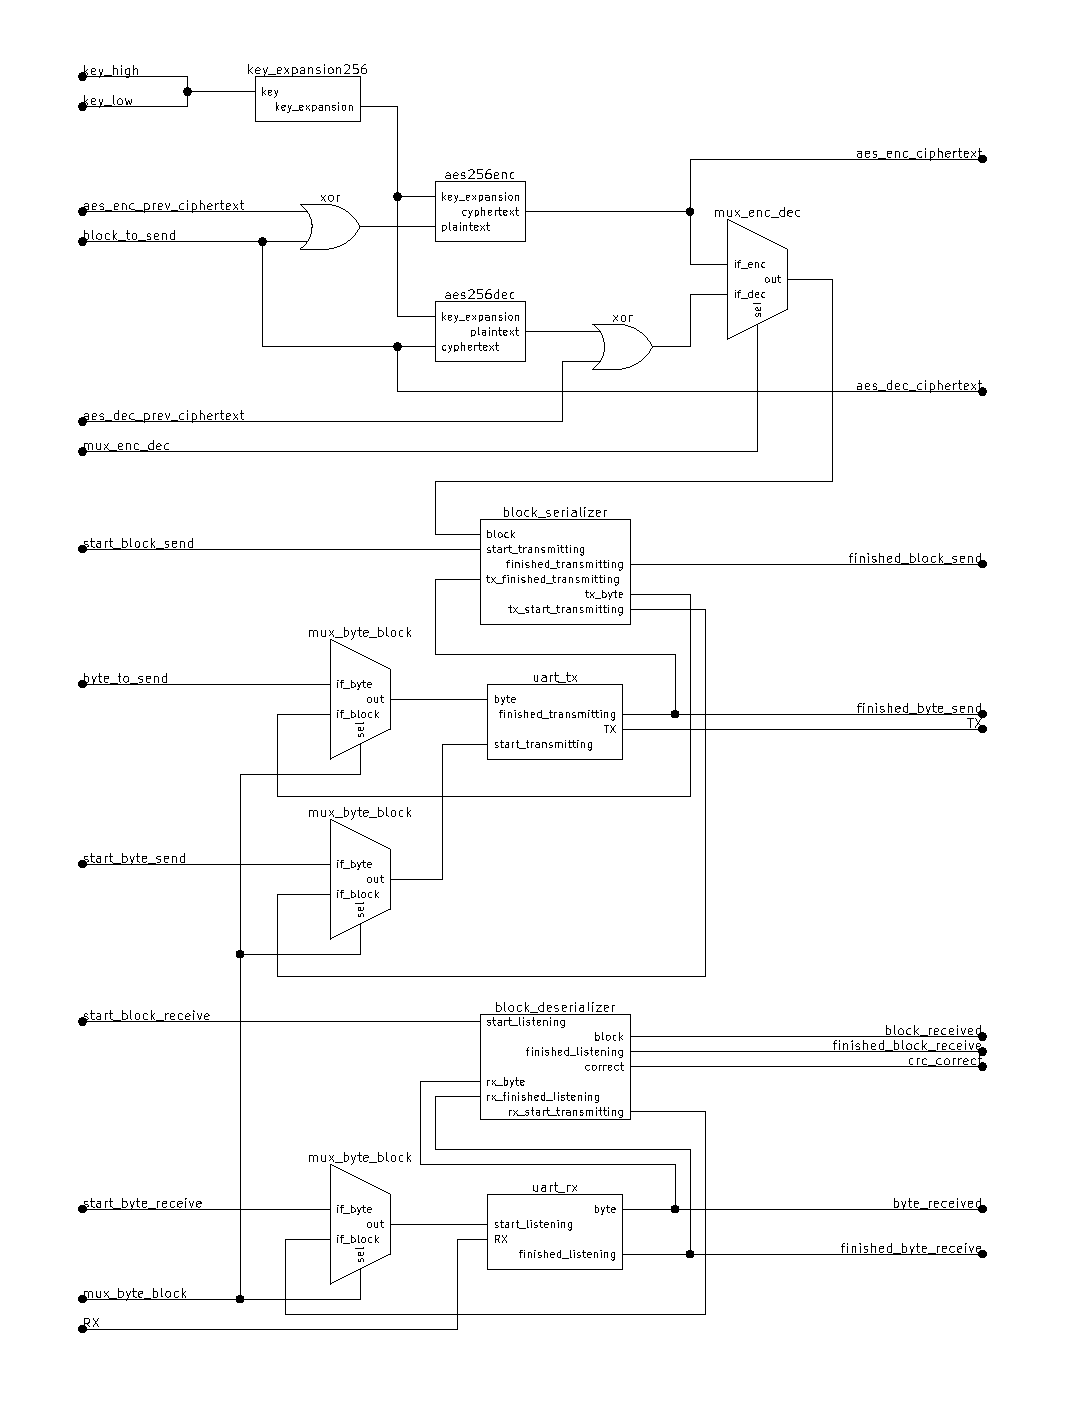
\includegraphics{pictures/communicator.pdf}
\caption{Schemat modułu \textit{communicator}}
\label{fig:communicator-schemat}
\end{figure}

%%%%%%%%%%%%%%%%%%%%%%%%%%%%%%%%%%%%%%%%%%%%%%%%%%%%%%%%%%%%%%%%%%%%%%%%%%%%%%%%%%%%%%%%%%%%%%%%%%%%%%%%
%%%%%%%%%%%%%%%%%%%%%%%%%%%%%%%%%%%%%%%%%%%%%%%%%%%%%%%%%%%%%%%%%%%%%%%%%%%%%%%%%%%%%%%%%%%%%%%%%%%%%%%%
%%%%%%%%%%%%%%%%%%%%%%%%%%%%%%%%%%%%%%%%%%%%%%%%%%%%%%%%%%%%%%%%%%%%%%%%%%%%%%%%%%%%%%%%%%%%%%%%%%%%%%%%


\newpage
\subsection{Skrypt klienta}
Skrypt klienta jest implementacją algorytmu komunikacji z serwerem szyfrującym (płytką Terasic DE1-SOC) przedstawionego w sekcji \ref{sec:przebieg-komunikacji}. Program przyjmuje od użytkownika tryb działania (szyfrowanie lub deszyfrowanie), klucz szyfrowania, wektor inicjalizacji oraz nazwy plików wejściowego i wyjściowego. Program odczytuje z dysku dane wejściowe, wysyła je do serwera oraz odbiera dane przetworzone i zapisuje je do pliku wynikowego. Jest napisany w języku python, oraz korzysta z bibliotek:
\begin{description}[noitemsep]
\item[serial] -- komunikacja przez port szeregowy UART
\item[threading] -- wielowątkowość związana z jednoczesnym wysyłaniem i odbieraniem bloków
\item[crcmod] -- obliczanie sumy kontrolnej crc16
\item[struct] -- konwersja liczby crc16 do tablicy bajtów możliwej do przesłania biblioteką serial
\item[argparse] -- parsowanie argumentów programu
\item[re] -- obsługa wyrażeń regularnych
\end{description}

\subsubsection{Padding}
Algorytm AES działa na blokach o wielkości 128b. W celu przetwarzania danych o wielkości nie będącej wielokrotnością rozmiaru bloku stosowany jest padding. W tym projekcie należy to do zadań klienta. Używany jest padding metodą dopełniania bloków do rozmiarów 128b bajtami o wartości równej brakującej liczbie bajtów. W celu uniknięcia niejednoznaczności przy usuwaniu wypełnienia, do wiadomości o wielkości będącej wielokrotnością 128b dodawany jest cały blok bajtów o wartości 16. W ten sposób ostatni bajt wiadomości zawsze zawiera liczbę bajtów dopełnienia, co pozwala na jednoznaczne usunięcie paddingu. 

Zastosowana metoda jest jedną ze standardowych praktyk. Została wybrana ze względu na fakt, że jest używana przez program \textit{openssl}, z którym produkt końcowy ma być kompatybilny. Jest zaimplementowana w sposób zgodny ze standardem RFC-2315 \cite{padding-rfc}.





\newpage
\section{Szczegóły implementacyjne -- AES}
\label{sec:szczegoly-implementacyjne-aes}
Szyfrowanie i deszyfrowanie jest realizowane w sposób zgodny ze standardem AES \cite{aes-standard}. Moduły szyfrujący i deszyfrujący działają w sposób asynchroniczny -- nie są taktowane zegarem. Takie rozwiązanie zostało wybrane ze względu na fakt, że wąskim gardłem systemu jest kanał komunikacji. Próby poprawy wydajności szyfrowania oraz deszyfrowania np. poprzez implementację przetwarzania potokowego (ang. \textit{pipelining}) nie przyniosłyby skutku ze względu na bardzo niską osiągalną prędkość transmisji (rozdz. \ref{sec:uart-parametry}).

Logika AES jest zaimplementowane w języku VHDL jako funkcje, które zostały zdekomponowane do niewielkich składowych w celu poprawy czytelności kodu.

\subsection{Arytmetyka w ciele \textit{GF($2^8$)}}
\label{sec:arytmetyka}
Transformacje stanu używane przez Algorytm AES są zdefiniowane przy pomocy działań na wielomianach o współczynnikach należących do ciała skończonego \textit{GF($2^8$)} \cite[rozdz. 4.3]{aes-standard}. Arytmetyka w tym ciele różni się od arytmetyki w ciele liczb rzeczywistych.

\paragraph{Dodawanie w ciele \textit{GF($2^8$)}} \cite[rozdz. 4.1]{aes-standard} jest operacją XOR. Takie działanie jest dostępne w języku VHDL, więc nie wymagało implementacji specjalnej procedury.

\paragraph{Mnożenie w ciele \textit{GF($2^8$)}} \cite[rozdz. 4.2]{aes-standard} jest równoważne mnożeniu wielomianów modulo pewien wielomian nierozkładalny -- dla AES jest to wielomian
\begin{equation*}
m(x) = x^8 + x^4 + x^3 + x + 1
\end{equation*}
To działanie jest zaimplementowane jako funkcja \textit{multiply}(listing \ref{lst:multiply-impl}) realizująca zmodyfikowany algorytm dodawania \textit{peasant's algorithm} \cite{multiply-algo}.

\begin{figure}[!h]
\begin{lstlisting}[style=vhdl, captionpos=b, caption={Mnożenie wielomianów w ciele \textit{GF($2^8$)}}, label={lst:multiply-impl}]
function multiply (left  : std_logic_vector(7 downto 0); 
                   right : std_logic_vector(7 downto 0)) 
return std_logic_vector is
	
constant irred_poly      : std_logic_vector(7 downto 0) := x"1b";
variable a               : std_logic_vector(7 downto 0) := (others => '0');
variable b               : std_logic_vector(7 downto 0) := (others => '0');
variable p               : std_logic_vector(7 downto 0) := (others => '0');
variable extended_b_lsb  : std_logic_vector(7 downto 0) := (others => '0');
variable extended_a_carry: std_logic_vector(7 downto 0) := (others => '0');

begin
	a := left;
	b := right;
	p := (others => '0');

	for i in 0 to 7 loop
		--1
		extended_b_lsb := (others => b(0));
		p := p xor (extended_b_lsb and a);

		--2
		b := '0' & b(7 downto 1);

		--3
		extended_a_carry := (others => a(7));

		--4
		a := a(6 downto 0) & '0';

		--5
		a := a xor (extended_a_carry and irred_poly);
	end loop;
		
	return p;
end function;
\end{lstlisting}
\end{figure}


\newpage
\subsection{Transformacje stanu}
Algorytm AES przy szyfrowaniu oraz rozwinięciu klucza wykorzystuje cztery podstawowe transformacje stanu.

\paragraph{SubBytes} \cite[rozdz. 5.1.1]{aes-standard} jest transformacją realizującą nieliniowe podstawienie bajtów. Każdy bajt stanu jest zastąpiony odpowiadającym mu bajtem \cite[rys. 6]{aes-standard} z tablicy podstawień S-Box \cite[rys. 7]{aes-standard}, która jest zaimplementowana jako tablica predefiniowanych stałych (listing. \ref{lst:s-box}). Pobranie z tablicy wartości do podstawienia realizowane jest przez funkcję \textit{lookup\_sub}. Transformacja SubBytes jest funkcją korzystającą ze zdefiniowanego S-Box (listing \ref{lst:sub-bytes}).

\paragraph{ShiftRows} \cite[rozdz. 5.1.2]{aes-standard} jest transformacją polegającą na cyklicznym przesunięciu trzech ostatnich rzędów stanu w lewo odpowiednio o 1, 2 lub 3 pozycje \cite[rys. 8]{aes-standard} (listing \ref{lst:shift-rows}).

\paragraph{AddRoundKey} \cite[rozdz. 5.1.3]{aes-standard} jest transformacją polegającą na dodaniu (operacja XOR, rozdz. \ref{sec:arytmetyka}) do stanu klucza rundy \cite[rys. 10]{aes-standard} (listing \ref{lst:add-round-key}). Wszystkie rundy posiadają oddzielne klucze, które są wygenerowane przy pomocy procedury rozwinięcia klucza (rozdz. \ref{sec:key-expansion}).

\paragraph{MixColumns} \cite[rozdz. 5.1.3]{aes-standard} jest transformacją operującą na kolumnach, która taktuje je jako wielomiany o współczynnikach należących do ciała \textit{GF($2^8$)}, będących wartościami odpowiednich bajtów stanu. Każda z kolumn jest pomnożona modulo $x^4 + 1$ przez wielomian $a(x)$ \cite[rys. 9]{aes-standard}.
\begin{equation*}
a(x) = 3x^3 + x^2 + x + 2
\end{equation*}
Transformacja MixColumns jest zaimplementowana jako funkcja modyfikująca stan według wzorów wyprowadzonych w dokumencie stanowiącym standard AES \cite[rozdz. 5.1.3]{aes-standard} (listing \ref{lst:mix-columns}).


\begin{figure}[!h]
\begin{lstlisting}[style=vhdl, captionpos=b, caption={Implementacja S-Box}, label={lst:s-box}]
type t_sub_table is array (0 to 255) of std_logic_vector(7 downto 0);

constant sub_table : t_sub_table := (
	------|   0      1      2      3      4      5     ...     e      f
	------|------|------|------|------|------|------|------|------|------|
	/* 0 */ x"63", x"7c", x"77", x"7b", x"f2", x"6b",  ... , x"ab", x"76",
	/* 1 */ x"ca", x"82", x"c9", x"7d", x"fa", x"59",  ... , x"72", x"c0",
	/* 2 */ x"b7", x"fd", x"93", x"26", x"36", x"3f",  ... , x"31", x"15",
	/* 3 */ x"04", x"c7", x"23", x"c3", x"18", x"96",  ... , x"b2", x"75",
	/* 4 */ x"09", x"83", x"2c", x"1a", x"1b", x"6e",  ... , x"2f", x"84",
	/* 5 */ x"53", x"d1", x"00", x"ed", x"20", x"fc",  ... , x"58", x"cf",
	/* 6 */ x"d0", x"ef", x"aa", x"fb", x"43", x"4d",  ... , x"9f", x"a8",
	/* 7 */ x"51", x"a3", x"40", x"8f", x"92", x"9d",  ... , x"f3", x"d2",
	/* 8 */ x"cd", x"0c", x"13", x"ec", x"5f", x"97",  ... , x"19", x"73",
	/* 9 */ x"60", x"81", x"4f", x"dc", x"22", x"2a",  ... , x"0b", x"db",
	/* a */ x"e0", x"32", x"3a", x"0a", x"49", x"06",  ... , x"e4", x"79",
	/* b */ x"e7", x"c8", x"37", x"6d", x"8d", x"d5",  ... , x"ae", x"08",
	/* c */ x"ba", x"78", x"25", x"2e", x"1c", x"a6",  ... , x"8b", x"8a",
	/* d */ x"70", x"3e", x"b5", x"66", x"48", x"03",  ... , x"1d", x"9e",
	/* e */ x"e1", x"f8", x"98", x"11", x"69", x"d9",  ... , x"28", x"df",
	/* f */ x"8c", x"a1", x"89", x"0d", x"bf", x"e6",  ... , x"bb", x"16");

function lookup_sub (index : std_logic_vector(7 downto 0)) 
return std_logic_vector is begin
	return sub_table(to_integer(unsigned(index)));
end function;
\end{lstlisting}
\end{figure}

\begin{figure}[!p]
\begin{lstlisting}[style=vhdl, captionpos=b, caption={Implementacja transformacji stanu SubBytes}, label={lst:sub-bytes}]
function sub_bytes (state_in : aes_state) return aes_state is 
	variable state_out : aes_state;
begin
	for r in 0 to 3 loop
		for c in 0 to 3 loop
			state_out(r, c) := lookup_sub(state_in(r, c));
		end loop;
	end loop;
		
	return state_out;
end function;
\end{lstlisting}
\end{figure}


\begin{figure}[!p]
\begin{lstlisting}[style=vhdl, captionpos=b, caption={Implementacja transformacji stanu ShiftRows}, label={lst:shift-rows}]
function shift_rows (state_in : aes_state) return aes_state is
 	variable state_out : aes_state;
begin
	for r in 0 to 3 loop
		for c in 0 to 3 loop
			state_out(r, c) := state_in(r, (c + r) mod 4);
		end loop;
	end loop;
		
	return state_out;
end function;
\end{lstlisting}
\end{figure}


\begin{figure}[!p]
\begin{lstlisting}[style=vhdl, captionpos=b, caption={Implementacja transformacji stanu AddRoundKey}, label={lst:add-round-key}]
function add_round_key state_in      : aes_state; 
                       key_expansion : std_logic_vector; 
                       round_number  : Integer) return aes_state is
	constant byte_bits   : Integer := 8;
	constant word_length : Integer := 4 * 8;
	constant Nb          : Integer := 4;

	variable key_word    : std_logic_vector(word_length - 1 downto 0);
 	variable state_out   : aes_state;
begin
	for c in 0 to 3 loop
		key_word := key_expansion((round_number * Nb + 1 + c) * word_length-1 
			downto (round_number * Nb + c) * word_length);
		for r in 0 to 3 loop
			state_out(r, c) := state_in(r, c) 
				xor key_word(byte_bits * (r + 1) - 1 downto byte_bits * r);
		end loop;
	end loop;

	return state_out;
end function;
\end{lstlisting}
\end{figure}

\begin{figure}[!t]
\begin{lstlisting}[style=vhdl, captionpos=b, caption={Implementacja transformacji stanu MixColumns}, label={lst:mix-columns}]
function mix_columns  state_in : aes_state) return aes_state is
	variable state_out : aes_state;
begin
	for c in 0 to 3 loop
		state_out(0, c) :=     multiply(x"02", state_in(0, c)) 
		                   xor multiply(x"03", state_in(1, c))
		                   xor                 state_in(2, c)  
		                   xor                 state_in(3, c);
				
		state_out(1, c) :=                     state_in(0, c)  
		                   xor multiply(x"02", state_in(1, c)) 
		                   xor multiply(x"03", state_in(2, c)) 
		                   xor                 state_in(3, c);
				
		state_out(2, c) :=                     state_in(0, c)  
		                   xor                 state_in(1, c)
		                   xor multiply(x"02", state_in(2, c)) 
		                   xor multiply(x"03", state_in(3, c));
		   			
		state_out(3, c) :=     multiply(x"03", state_in(0, c)) 
		                   xor                 state_in(1, c)
		                   xor                 state_in(2, c)  
		                   xor multiply(x"02", state_in(3, c));
	end loop;

	return state_out;
end;
\end{lstlisting}
\end{figure}

\newpage
\subsection{Rozwinięcie klucza}
\label{sec:key-expansion}
Algorytm AES w każdej rundzie potrzebuje osobnego 128-bitowego klucza rundy. Aby otrzymać te klucze rozwija się 256-bitowy klucz szyfrowania przy pomocy algorytmu Rijndael'a (ang. \textit{Rijndael key schedule}) \cite[rozdz. 5.2]{aes-standard}. Procedura została zaimplementowana jako funkcja (listing \ref{lst:key-schedule}) działająca według algorytmu opisanego w standardzie AES \cite[rys. 11]{aes-standard}.

\begin{figure}[!p]
\begin{lstlisting}[style=vhdl, captionpos=b, caption={Implementacja rozwinięcia klucza -- \textit{Rijndael key schedule}}, label={lst:key-schedule}]
function key_expansion256 (key : std_logic_vector) 
return std_logic_vector is

constant word_length : Integer := 4 * 8;
constant byte_bits   : Integer := 8;
constant Nk          : Integer := 8;
	
variable tmp         : std_logic_vector(word_length - 1 downto 0);
variable tmp2        : std_logic_vector(word_length - 1 downto 0);
variable rcon        : std_logic_vector(word_length - 1 downto 0);
variable result      : std_logic_vector(60 * word_length - 1 downto 0);

begin

result(word_length * Nk - 1 downto 0) := key;
for i in Nk to 59 loop
	tmp := result(word_length * i - 1 downto word_length * (i - 1));
	
	if (i mod Nk = 0) then
		--RotWord
		tmp2 := tmp;
		tmp(word_length - 1 downto word_length - byte_bits) := 
			tmp2(byte_bits - 1 downto 0);
		tmp(word_length - byte_bits - 1 downto 0) := 
			tmp2(word_length - 1 downto byte_bits);

		--SubWord
		for j in 0 to 3 loop
			tmp((j + 1) * byte_bits - 1 downto j * byte_bits) := 
				lookup_sub(tmp((j + 1) * byte_bits - 1 downto j * byte_bits));
		end loop;

		--Rcon XOR
		tmp(byte_bits - 1 downto 0) := 
			tmp(byte_bits - 1 downto 0) 
			  xor std_logic_vector(to_unsigned(2 ** (i / Nk - 1), byte_bits));

	elsif (i mod Nk = 4) then
		--SubWord
		for j in 0 to 3 loop
			tmp((j + 1) * byte_bits - 1 downto j * byte_bits) := 
				lookup_sub(tmp((j + 1) * byte_bits - 1 downto j * byte_bits));
		end loop;
	end if;
	
	result(word_length * (i + 1) - 1 downto word_length * i) := 
		tmp xor result(word_length * (i-Nk+1)-1 downto word_length * (i-Nk));
end loop;
return result;

end function;
\end{lstlisting}
\end{figure}

\newpage
\subsection{Moduł szyfrujący AES}
Logika szyfrująca została zaimplementowana jako funkcja realizująca algorytm opisany w standardzie AES \cite[rozdz. 5.1, rys. 5]{aes-standard} (listing \ref{lst:aes-encryption}). Korzysta ona ze zdefiniowanych funkcji pomocniczych wykonujących kolejne rundy przekształcenia (listing \ref{lst:rounds}).

Moduł szyfrujący AES przyjmuje rozwinięcie klucza i blok tekstu jawnego oraz zwraca tekst zaszyfrowany. Jest zaimplementowany jako wywołanie funkcji szyfrującej (listing. \ref{lst:aes-encryption-module}).

Opis sygnałów interfejsu modułu \textit{aes256enc}:
\begin{interface}{KEY\_EXPANSION}
	\item[\insignal{KEY\_EXPANSION}] rozwinięcie klucza AES.
	\item[\insignal{PLAINTEXT}] blok tekstu jawnego.
	\item[\outsignal{CYPHERTEXT}] blok tekstu zaszyfrowanego.
\end{interface}

\begin{figure}[!h]
\begin{lstlisting}[style=vhdl, captionpos=b, caption={Implementacja funkcji szyfrującej AES}, label={lst:aes-encryption}]
function encode256 (plaintext     : std_logic_vector; 
                    key_expansion : std_logic_vector) 
return std_logic_vector is
	variable cyphertext    : std_logic_vector(127 downto 0);
	variable state         : aes_state;
	begin
	for r in 0 to 3 loop
		for c in 0 to 3 loop
			state(r, c) := plaintext((r + 4 * c + 1) * 8-1 downto (r+4*c)*8);
		end loop;
	end loop;

	state := round_0(state, key_expansion);

	for i in 1 to 13 loop
		state := round_n(state, key_expansion, i);
	end loop;

	state := round_last(state, key_expansion);

	for r in 0 to 3 loop
		for c in 0 to 3 loop
			cyphertext((r + 4 * c + 1) * 8-1 downto (r+4*c)*8) := state(r, c);
		end loop;
	end loop;

	return cyphertext;
end function;
\end{lstlisting}
\end{figure}

\begin{figure}[!p]
\begin{lstlisting}[style=vhdl, captionpos=b, caption={Implementacja rund szyfrowania}, label={lst:rounds}]
function round_0 (state_in      : aes_state; 
                  key_expansion : std_logic_vector) return aes_state is begin
	return add_round_key(state_in, key_expansion, 0);
end function;

function round_n (state_in      : aes_state; 
                  key_expansion : std_logic_vector;
                  n             : Integer) return aes_state is
	variable state : aes_state;
begin
	state := state_in;
	state := sub_bytes(state);
	state := shift_rows(state);
	state := mix_columns(state);
	state := add_round_key(state, key_expansion, n);

	return state;
end function;

function round_last (state_in      : aes_state; 
                     key_expansion : std_logic_vector) return aes_state is
	variable state : aes_state;
begin
	state := state_in;
	state := sub_bytes(state);
	state := shift_rows(state);
	state := add_round_key(state, key_expansion, 14);

	return state;
end function;
\end{lstlisting}
\end{figure}

\begin{figure}[!p]
\begin{lstlisting}[style=vhdl, captionpos=b, caption={\textit{aes256enc} -- interfejs i implementacja modułu szyfrującego AES}, label={lst:aes-encryption-module}]
entity aes256enc is
	generic (
		byte_bits          : Integer := 8;
		block_bytes        : Integer := 16;
		block_bits         : Integer := 128;
		key_bytes          : Integer := 32;
		key_expansion_bits : Integer := 15 * 128);
	port (
		key_expansion : in  std_logic_vector(key_expansion_bits-1 downto 0);
		plaintext     : in  std_logic_vector(block_bits - 1 downto 0);
		cyphertext    : out std_logic_vector(block_bits - 1 downto 0));
end aes256enc;

architecture aes256enc_impl of aes256enc is begin

	cyphertext <= encode256(plaintext, key_expansion);

end aes256enc_impl;
\end{lstlisting}
\end{figure}




\newpage
\subsection{Moduł deszyfrujący AES}
Moduł deszyfrujący AES przyjmuje rozwinięcie klucza i blok tekstu zaszyfrowanego oraz zwraca blok tekstu jawnego.

\begin{figure}[!h]
\begin{lstlisting}[style=vhdl, captionpos=b, caption={\textit{aes256dec} -- interfejs i implementacja modułu deszyfrującego AES}, label={lst:aes-decryption-module}]
port (
	key_expansion : in  std_logic_vector(key_expansion_bits - 1 downto 0);
	cyphertext    : in  std_logic_vector(block_bits - 1 downto 0);
	plaintext     : out std_logic_vector(block_bits - 1 downto 0));
\end{lstlisting}
\end{figure}

Opis sygnałów interfejsu modułu \textit{aes256dec}:
\begin{interface}{KEY\_EXPANSION}
	\item[\insignal{KEY\_EXPANSION}] rozwinięcie klucza AES.
	\item[\insignal{CYPHERTEXT}] blok tekstu zaszyfrowanego.
	\item[\outsignal{PLAINTEXT}] blok tekstu jawnego.
\end{interface}

Podczas deszyfrowania wykorzystywane są transformacje odwrotne \cite[rozdz. 5.3.1-4]{aes-standard}. Kolejność przekształceń w rundach również jest inna \cite[rys. 12]{aes-standard}. Funkcja deszyfrująca oraz wszystkie jej składowe zostały zaimplementowane analogicznie do ich szyfrujących odpowiedników, zgodnie ze standardem AES \cite[rozdz. 5.3]{aes-standard}.

\subsection{Tryb wiązania bloków CBC}
W celu zaszyfrowania danych o wielkości przekraczającej 128b konieczny jest ich podział na bloki. Jeśli każdy z otrzymanych bloków zostanie zaszyfrowany niezależnie (w trybie ECB \cite{cbc-comparison}) może to prowadzić do luk w bezpieczeństwie. Jest to następstwem faktu, że postaci zaszyfrowane jednakowych bloków są równe. Jest to zauważalne np. dla obrazów (rys. \ref{fig:cbc-comparison}).

\begin{figure}[!h]
\subfloat[Postać jawna]{
\includegraphics[width = 2 in]{pictures/duck-plaintext.jpg}}
\hfill
\subfloat[Bloki szyfrowane niezależnie]{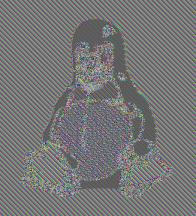
\includegraphics[width = 2 in]{pictures/duck-ecb.jpg}}
\hfill
\subfloat[Tryb CBC]{
\includegraphics[width = 2 in]{pictures/duck-cbc.jpg}}
\caption{Wpływ trybu CBC na wynik szyfrowania \cite{cbc-comparison}}
\label{fig:cbc-comparison}
\end{figure}

Aby zapobiec takim lukom w bezpieczeństwie stosowane są tryby wiązania bloków. W tym projekcie używany jest tryb CBC (ang. \textit{cipher block chaining}), który został wybrany ze względu na jego dużą popularność. Polega on na dodawaniu (operacja XOR) do bloków tekstu jawnego postaci zaszyfrowanych bloków poprzedzających (rys. \ref{fig:cbc}). W celu szyfrowania pierwszego bloku stosowany jest wektor inicjalizacji.

\begin{figure}[!h]
\centering
\subfloat[Szyfrowanie w trybie CBC]{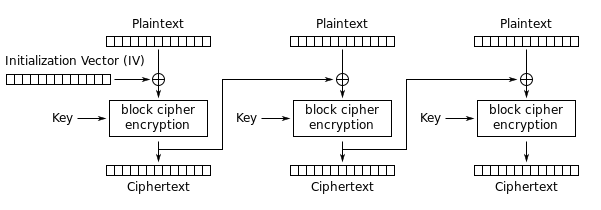
\includegraphics[width = \textwidth]{pictures/cbc-encryption.png}}
\newline
\subfloat[Deszyfrownaie w trybie CBC]{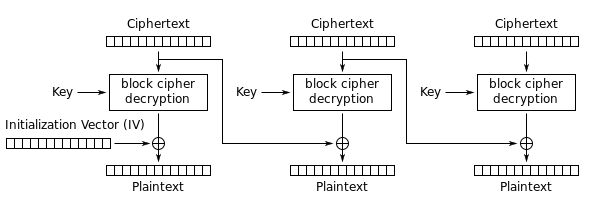
\includegraphics[width = \textwidth]{pictures/cbc-decryption.png}}
\caption{Sposób działania trybu wiązania bloków CBC \cite{cbc}}
\label{fig:cbc}
\end{figure}

Wiązanie boków w trybie CBC jest realizowane przez moduł \textit{communicator} (rozdz. \ref{sec:comminicator}). Operacja zaimplementowana jest przy pomocy bramek XOR:
\begin{itemize}
\item W przypadku szyfrowania bramka sumuje sygnał bloku do zaszyfrowania z zaszyfrowaną postacią bloku poprzedniego (lub wektorem inicjalizacji dla bloku pierwszego). Sygnał wyjściowy bramki połączony jest bezpośrednio do wejścia \textit{plaintext} modułu \textit{aes256enc} (rys. \ref{fig:communicator-schemat}).
\item W przypadku deszyfrowania bramka sumuje sygnał wyjściowy \textit{plaintext} modułu \textit{aes256dec} z zaszyfrowaną postacią bloku poprzedniego (lub wektorem inicjalizacji w przypadku bloku pierwszego). Sygnał wyjściowy bramki interpretowany jest jako postać jawna bloku (rys. \ref{fig:communicator-schemat}).
\end{itemize}
\section{Szczegóły implementacyjne -- komunikacja}
\label{sec:szczegoly-implementacyjne-uart}
Komunikacja między klientem (komputerem PC) a serwerem (płytką z układem FPGA) jest realizowana zgodnie z protokołem UART. Zaimplementowane zostały moduły odpowiadające za obsługę takiej komunikacji. Stworzone zostały również moduły odbierające i wysyłające bloki AES, oraz sterujące procesem komunikacji, kontroli błędów oraz szyfrowania i deszyfrowania.

\subsubsection{Moduł odbierający bajty UART}
Interfejs układu odbierającego bajty UART \textit{uart\_rx}:

\begin{interface}{FINISHED\_LISTENING}
	\item[\insignal{CLK\_16}] główny zegar układu.
	\item[\insignal{RX}] zsynchronizowany przy pomocy dwóch przerzutników typu D sygnał UART RX, wychodzący z konwertera USB-UART.
	\item[\insignal{START\_LISTENING}] sygnał wprowadzający komponent w stan oczekiwania na bajt.
	\item[\outsignal{BYTE[7:0]}] odebrany bajt. Stabilność sygnału jest gwarantowana, gdy \outsignal{FINISHED\_LISTENING} jest w stanie wysokim.
	\item[\outsignal{FINISHED\_LISTENING}] sygnał informujący o zakończeniu odbierania bajtu oraz gotowość na otrzymanie kolejnego sygnału \insignal{START\_LISTENING} podczas kolejnego zbocza rosnącego zegara \insignal{CLK\_16}.
\end{interface}

Po otrzymaniu sygnału \insignal{START\_LISTENING} moduł rozpoczyna nasłuchiwanie na transmisję. Każdy bit jest próbkowany 16 razy. Wartość bitu jest ustalana na podstawie \textit{głosowania} -- bit jest uznawany za {'1'} jeśli co najmniej dwie z trzech środkowych próbek mają wartość {'1'}, analogicznie dla {'0'}. Transmisja bajtu zostaje uznana za rozpoczętą, jeśli zostanie odebrany bit startu -- gdy zostanie napotkana pierwsza próbka o wartości {'0'} i potwierdzona przez głosowanie. Bajt zostaje uznany za poprawnie odebrany, jeśli zostanie odebrany poprawny bit stopu. Bit stopu jest próbkowany jedynie 9 razy. Jest to minimalna liczba próbek pozwalająca przeprowadzić \textit{głosowanie}. Próbkowanie bitu stopu jest skrócone, ze względu na fakt, że pomimo ustawienia zgodnych parametrów transmisji nadajnika i odbiornika, zegar urządzenia nadającego może być minimalnie szybszy. Prowadzi to do zbyt wolnego odbierania napływających informacji i po kilku odebranych bajtach prowadzi do błędów, co zostało zaobserwowane w trakcie testów. Skrócenie czasu odbierania bitu stopu zapobiega takim sytuacjom.

\begin{figure}[!h]
	\centering
	\begin{tikztimingtable}
	\insignal{CLK\_16}          & 32{cc}  \\
	\insignal{RX}               & HHH    16J{Start}    13D{Data[0]}\\
	\insignal{START\_LISTENING} & LH30L\\
	\extracode
	\tablerules
	\draw[red, ->] (3.5,0) -- (3.5,1);
	\draw[red, ->] (9.5,0) -- (9.5,1);
	\draw[red, ->] (10.5,0) -- (10.5,1);
	\draw[red, ->] (11.5,0) -- (11.5,1);
	\draw[red, ->] (26.5,0) -- (26.5,1);
	\draw[red, ->] (27.5,0) -- (27.5,1);
	\draw[red, ->] (28.5,0) -- (28.5,1);
	\end{tikztimingtable}
\caption{\textit{uart\_rx} -- odbiór bitu startu}
\end{figure}

\begin{figure}[!h]
	\centering
	\begin{tikztimingtable}
	\insignal{CLK\_16}              & 31{cc}  \\
	\insignal{RX}                   & 13D{Data[7]} 16J{Stop} HH   \\
	\outsignal{BYTE[7:0]}           & 22U D 8U \\
	\outsignal{FINISHED\_LISTENING} & 22L H 8L \\
	\extracode
	\tablerules
	\draw[red, ->] (4.5,0) -- (4.5,1);
	\draw[red, ->] (5.5,0) -- (5.5,1);
	\draw[red, ->] (3.5,0) -- (3.5,1);
	\draw[red, ->] (19.5,0) -- (19.5,1);
	\draw[red, ->] (20.5,0) -- (20.5,1);
	\draw[red, ->] (21.5,0) -- (21.5,1);
	\end{tikztimingtable}
\caption{\textit{uart\_rx} -- odbiór bitu stopu}
\end{figure}

\begin{figure}[!h]
	\centering
	\begin{tikztimingtable}[timing/wscale=2.8]
  	\insignal{CLK\_UART}            & c cc        cc         cc         cc         cc         cc         cc         cc         cc         cc       c \\
  	\insignal{RX}                   & u J{Start}  D{Data[0]} D{Data[1]} D{Data[2]} D{Data[3]} D{Data[4]} D{Data[5]} D{Data[6]} D{Data[7]} K{Stop}  u \\
  	\outsignal{BYTE[7:0]}           & 10U 0.5d 1.5u \\
	\outsignal{FINISHED\_LISTENING} & 10L 0.5h 1.5l \\
	\extracode
	\tablerules
	\end{tikztimingtable}
\caption{\textit{uart\_rx} -- odbiór całej ramki UART}
\end{figure}
\newpage
\subsection{Moduł wysyłający bajty UART}
Moduł \textit{uart\_tx} wysyła bajty do klienta przez interfejs UART.

\begin{figure}[!h]
\begin{lstlisting}[style=vhdl, captionpos=b, caption={\textit{uart\_tx} -- interfejs modułu}]
port (
	reset_n               : in  std_logic;
	clk_16                : in  std_logic;
	tx                    : out std_logic;

	byte                  : in  std_logic_vector(byte_bits - 1 downto 0);
	start_transmitting    : in  std_logic;
	finished_transmitting : out std_logic);
\end{lstlisting}
\end{figure}

Opis sygnałów interfejsu modułu \textit{uart\_tx}:
\begin{interface}{FINISHED\_TRANSMITTING}
\item[\insignal{CLK\_16}] główny zegar układu.
\item[\insignal{START\_TRANSMITTING}] sygnał rozpoczynający wysyłanie danych.
\item[\insignal{BYTE[7:0]}] bajt do wysłania. Stabilność sygnału jest wymagana, gdy \insignal{START\_TRANSMITTING} jest w stanie wysokim.
\item[\outsignal{TX}] sygnał UART TX wychodzący do konwertera USB-UART.
\item[\outsignal{FINISHED\_TRANSMITTING}] sygnał sygnalizujący zakończenie wysyłania bajtu oraz gotowość na otrzymanie kolejnego sygnału \insignal{START\_TRANSMITTING} podczas kolejnego zbocza rosnącego.
\end{interface}

Moduł rozpoczyna transmisję po otrzymaniu sygnału \insignal{START\_TRANSMITTING} (rys. \ref{fig:uart-tx-stop-start}). Wysyłany jest bajt (rys. \ref{fig:uart-tx-frame}) dostarczony do modułu przez sygnał \insignal{BYTE[7:0]}. Bity startu, danych oraz stopu są wysyłane przez 16 cykli zegara \insignal{CLK\_16}. Zakończenie wysyłania ramki UART sygnalizowane jest przez sygnał \outsignal{FINISHED\_TRANSMITTING}, który również oznacza gotowość modułu na rozpoczęcie transmisji kolejnego bitu podczas następnego zbocza rosnącego. Sygnał \outsignal{FINISHED\_TRANSMITTING} wysyłany jest w przedostatnim cyklu zegarowym wysyłania bitu stopu, aby w ostatnim cyklu mógł nadejść następny sygnał \insignal{START\_TRANSMITTING}. Takie rozwiązanie umożliwia prowadzenie transmisji przez moduł z maksymalną możliwą prędkością -- ani jeden cykl zegara nie jest zmarnowany (rys. \ref{fig:uart-tx-stop-start}).

\newpage

\begin{center}
\centering
\resizebox{\textwidth}{!}{
	\begin{tikztimingtable}[timing/wscale=0.9]
	\insignal{CLK\_16}          & 3{cc}       16{cc}     16{cc}     3{cc}\\
	\insignal{START\_TRANS}     & 3U          15UH       16U        3U     \\
	\insignal{BYTE[7:0]}        & 3U          15UD       16U        3U          \\
	\outsignal{TX}              & 3D{Data[7]} 17.777K{Stop}  17.777J{Start} 3D{Data[0]}\\ %to offset crapy scaling
	\outsignal{FINISHED\_TRANS} & 3U          14UHU      16U        3U\\
	\extracode
	\tablerules
	\end{tikztimingtable}
}
\captionof{figure}{\textit{uart\_tx} -- wysłanie bitu stopu i startu}
\label{fig:uart-tx-stop-start}
\end{center}


\begin{center}
\centering
\resizebox{\textwidth}{!}{
	\begin{tikztimingtable}[timing/wscale=3.0]
	\insignal{CLK\_16}          & c              cc        cc         cc         cc         cc         cc         cc         cc         cc         cc       c \\
	\insignal{START\_TRANS}     & 0.5u0.5h 10.5U     \\
	\insignal{BYTE[7:0]}        & 0.5u0.5d 10.5U      \\
	\outsignal{TX}              & u              J{Start}  D{Data[0]} D{Data[1]} D{Data[2]} D{Data[3]} D{Data[4]} D{Data[5]} D{Data[6]} D{Data[7]} K{Stop}  u \\
	\outsignal{FINISHED\_TRANS} & u              9.5U 0.5h 1.5u\\
	\extracode
	\tablerules
	\end{tikztimingtable}
}
\captionof{figure}{\textit{uart\_tx} -- wysłanie całej ramki UART}
\label{fig:uart-tx-frame}
\end{center}
\subsubsection{Moduł deserializujący bajty UART do bloków AES}
Interfejs modułu deserializującego bajty UART do bloków AES \textit{block\_deserializer}:
\begin{interface}{RX\_FINISHED\_LISTENING}
	\item[\insignal{CLK\_16}] główny zegar układu.

	\item[\insignal{RX\_BYTE[7:0]}] sygnał pochodzący z komponentu \textit{uart\_rx}.
	\item[\outsignal{RX\_START\_LISTENING}] sygnał wychodzący do komponentu \textit{uart\_rx}.
	\item[\insignal{RX\_FINISHED\_LISTENING}] sygnał pochodzący z komponentu \textit{uart\_rx}.

	\item[\insignal{START\_LISTENING}] sygnał wprowadzający komponent w stan oczekiwania na blok.
	\item[\outsignal{BLOCK[127:0]}] odebrany blok AES. Stabilność sygnału jest gwarantowana, gdy \outsignal{FINISHED\_LISTENING} jest w stanie wysokim.
	\item[\outsignal{FINISHED\_LISTENING}] sygnał informujący o zakończeniu odbierania bloku AES oraz gotowość na otrzymanie kolejnego sygnału \insignal{START\_LISTENING} podczas następnego zbocza rosnącego zegara \insignal{CLK\_16}.
	\item[\outsignal{CORRECT}] sygnał określający, czy transmisja bloku AES przebiegła bez błędów. Stabilność sygnału jest gwarantowana, gdy \outsignal{FINISHED\_LISTENING} jest w stanie wysokim.
\end{interface}

Po otrzymaniu sygnału \insignal{START\_LISTENING} moduł rozpoczyna nasłuchiwanie na transmisję. Odbieranie bajtów bloku danych wykonywane jest przez przez moduł \textit{uart\_rx}. Kolejność ułożenia bajtów w bloku \outsignal{BLOCK[127:0]} jest zgodna ze standardem AES. W trakcie odbierania obliczana jest suma kontrolna \textit{CRC16}. Po 128 bajtach bloku danych przesyłane są 2 bajty zawierające oczekiwaną, obliczoną po stronie klienta sumę kontrolną. Jeśli jest ona zgodna z tą obliczaną na bieżąco przez moduł, sygnał \outsignal{CORRECT} przyjmuje wartość {'1'}, w przeciwnym wypadku wartość {'0'}. Po odebraniu 130 bajtów moduł zwraca blok \outsignal{BLOCK[127:0]} wraz z informacją o jego poprawności \outsignal{CORRECT} oraz sygnalizuje gotowość na rozpoczęcie nasłuchiwania na kolejne bloki \outsignal{FINISHED\_LISTENING}.

\begin{figure}[!h]
	\centering
	\begin{tikztimingtable}[timing/wscale=0.95]
	\insignal{CLK\_16}          & 3{cc}  16{cc}           16{cc}         \\
	\outsignal{RX\_START\_LIST} & LH     15LH             15LH           L\\
	\insignal{RX\_BYTE[7:0]}    & L      15LD{BLOCK[0]}   15LD{BLOCK[1]} 2L\\
	\insignal{RX\_FIN\_LIST}    & L      15LH             15LH           2L\\
	\insignal{START\_LIST}      & LH     16L              16L            L\\
	\extracode
	\tablerules
	\end{tikztimingtable}
\caption{\textit{block\_deserializer} -- rozpoczęcie odbierania}
\end{figure}

\begin{figure}[!h]
	\centering
	\begin{tikztimingtable}[timing/wscale=0.95]
	\insignal{CLK\_16}          & 3{cc}          16{cc}       16{cc}             \\
	\outsignal{RX\_START\_LIST} & 2LH            15LH         16L                \\
	\insignal{RX\_BYTE[7:0]}    & LD{BLOCK[127]} 15LD{CRC[0]} 15LD{CRC[1]}       L\\
	\insignal{RX\_FIN\_LIST}    & LH             15LH         15LH               L\\
	\outsignal{BLOCK[127:0]}    & 3L             15L          15LD{BLOCK[127:0]} L\\
	\outsignal{FIN\_LIST}       & 3L             15L          15LH               L\\
	\outsignal{CORRECT}         & 3L             15L          15LH               L\\
	\extracode
	\tablerules
	\end{tikztimingtable}
\caption{\textit{block\_deserializer} -- zakończenie odbierania}
\end{figure}

\begin{figure}[!h]
	\centering
	\begin{tikztimingtable}
	\helpsignal{CLK\_UART}      & 1.5l  130{0.25c0.25c}    l \\
	\outsignal{RX\_START\_LIST} & l     130{0.5lg}      1.5l \\
	\insignal{RX\_BYTE[7:0]}    & 1.5l  130{0.5lg}         l \\
	\insignal{RX\_FIN\_LIST}    & 1.5l  130{0.5lg}         l \\
	\insignal{START\_LIST}      & l         0.5lg        66l \\
	\outsignal{BLOCK[127:0]}    & 66.5l         g          l \\
	\outsignal{FIN\_LIST}       & 66.5l         g          l \\
	\outsignal{CORRECT}         & 66.5l         g          l \\
	\extracode
	\tablerules
	\end{tikztimingtable}
\caption{\textit{block\_deserializer} -- odbieranie całego bloku}
\end{figure}



\subsubsection{Moduł serializujący bloki AES do bajtów UART}
Interfejs modułu serializującego bloki AES do bajtów UART \textit{block\_serializer}:
\begin{interface}{RX\_FINISHED\_TRANSMITTING}
	\item[\insignal{CLK\_16}] główny zegar układu.

	\item[\insignal{TX\_BYTE[7:0]}] sygnał wychodzący do komponentu \textit{uart\_tx}.
	\item[\outsignal{TX\_START\_TRANSMITTING}] sygnał pochodzący z komponentu \textit{uart\_tx}.
	\item[\insignal{TX\_FINISHED\_TRANSMITTING}] sygnał wychodzący do komponentu \textit{uart\_tx}.

	\item[\insignal{START\_TRANSMITTING}] sygnał rozpoczynający transmisję bloku.
	\item[\insignal{BLOCK[127:0]}] blok AES do wysłania. Stabilność sygnału jest wymagana, gdy \outsignal{START\_TRANSMITTING} jest w stanie wysokim.
	\item[\outsignal{FINISHED\_TRANSMITTING}] sygnał informujący o zakończeniu wysyłania bloku AES oraz gotowość na otrzymanie kolejnego sygnału \insignal{START\_TRANSMITTING} podczas kolejnego zbocza rosnącego zegara \insignal{CLK\_16}.
\end{interface}

Po otrzymaniu sygnału \insignal{START\_TRANSMITTING} moduł rozpoczyna transmisję. Wysyłanie bajtów bloku danych wykonywane jest przez przez moduł \textit{uart\_tx}. Kolejność wysyłanych bajtów jest zgodna z kolejnością ich odbierania przez moduł \textit{block\_deserializer}. W trakcie wysyłania obliczana jest suma kontrolna \textit{CRC16}. Po 128 bajtach bloku danych wysyłane są 2 bajty zawierające obliczoną sumę kontrolną. Po wysłaniu 130 bajtów moduł sygnalizuje gotowość na rozpoczęcie transmisji kolejnego bloku \outsignal{FINISHED\_LISTENING}.

\begin{figure}[!h]
	\centering
	\begin{tikztimingtable}[timing/wscale=0.95]
	\insignal{CLK\_16}           & 3{cc}            16{cc}           16{cc}         \\
	\outsignal{TX\_START\_TRANS} & LH               15LH             15LH           L\\
	\outsignal{TX\_BYTE[7:0]}    & LD{BLOCK[0]}     15LD{BLOCK[1]}   15LD{BLOCK[2]} L\\
	\insignal{TX\_FIN\_TRANS}    & L                15LH             15LH           2L\\
	\insignal{BLOCK[127:0]}      & LD{BLOCK[127:0]} 16L              16L            L\\
	\insignal{START\_TRANS}      & LH               16L              16L            L\\
	\extracode
	\tablerules
	\end{tikztimingtable}
\caption{\textit{block\_serializer} -- rozpoczęcie wysyłania}
\end{figure}

\begin{figure}[!h]
	\centering
	\begin{tikztimingtable}[timing/wscale=0.95]
	\helpsignal{CLK\_16}         & 3{cc}           16{cc}       16{cc}  \\
	\outsignal{TX\_START\_TRANS} & 2LH             15LH         16L     \\
	\outsignal{TX\_BYTE[7:0]}    & 2LD{CRC[0]}     15LD{CRC[1]} 16L     \\
	\insignal{TX\_FIN\_TRANS}    & LH              15LH         15LH    L\\
	\outsignal{FIN\_TRANS}       & 2L              16L          15LH    L\\
	\extracode
	\tablerules
	\end{tikztimingtable}
\caption{\textit{block\_serializer} -- zakończenie wysyłania}
\end{figure}

\begin{figure}[!h]
	\centering
	\begin{tikztimingtable}
	\helpsignal{CLK\_UART}       & 1.5l  130{0.25c0.25c}    l \\
	\outsignal{TX\_START\_TRANS} & l     130{0.5lg}      1.5l \\
	\outsignal{TX\_BYTE[7:0]}    & l     130{0.5lg}      1.5l \\
	\insignal{TX\_FIN\_TRANS}    & 1.5l  130{0.5lg}         l \\
	\insignal{START\_TRANS}      & l         0.5lg        66l \\
	\insignal{BLOCK[127:0]}      & l         0.5lg        66l \\
	\outsignal{FIN\_TRANS}       & 66.5l         g          l \\
	\extracode
	\tablerules
	\end{tikztimingtable}
\caption{\textit{block\_serializer} -- transmisja całego bloku}
\end{figure}







\subsubsection{CRC16}
Do sprawdzania poprawności przesyłanych bloków używana jest suma kontrolna CRC16 -- wariant z wielomianem \textit{x8005}. Moduły \textit{block\_serializer} oraz \textit{block\_deserializer} zawierają zmienne wielkości 16b będące akumulatorami przechowującymi aktualnie obliczoną sumę CRC16. Przed rozpoczęciem transmisji są one zerowane. Każdy odebrany/wysłany bajt bloku danych aktualizuje akumulator zgodnie ze sposobem działania CRC16. Moduł \textit{block\_serializer} po wysłaniu bloku danych wysyła 2 bajty akumulatora będące sumą kontrolną bloku. Moduł \textit{block\_serializer} po odebraniu bloku, odbiera 2 bajty sumy kontrolnej obliczonej przez klienta, oraz dodaje je do akumulatora w taki sam sposób jak pozostałe bajty. Poprawność jest określana poprzez sprawdzenie, czy wszystkie bity akumulatora są równe {'0'} -- jeśli są to znaczy, że blok został odebrany poprawnie.

\begin{figure}[!h]
\begin{lstlisting}[language=Python, basicstyle=\ttfamily, autogobble=true, tabsize=3, morekeywords={downto, val, var}]
val crc_poly[16:0] := "1'1000'0000'0000'0101" # wielomian x8005

def crc_add(acc[15:0], data[7:0]):
	var tmp[23:0]

	tmp[23:8] := acc[15:0]
	tmp[7:0]  := data[7:0]

	for i in 23 downto 16:
		if tmp[i] == '1':
			tmp[i:i-16] := tmp[i:i-16] xor crc_poly[16:0]

	return tmp[15:0]
\end{lstlisting}
\caption{Algorytm dodawania bajtu do akumulatora sumy kontrolnej CRC16}
\end{figure}
\subsection{Moduł zarządzający komunikacją z klientem}
\label{sec:comminicator}
Moduł \textit{communicator} zarządza procesem komunikacji z klientem oraz kontroli poprawności przesyłanych danych. Zadaniem modułu jest realizacja serwerowej części ustalonego protokołu komunikacji z klientem (rozdz. \ref{sec:przebieg-komunikacji}), w szczególności:
\begin{itemize}[noitemsep, nolistsep]
\item zarządzanie procesem przesyłania bloków i potwierdzeń
\item kontrola poprawności bloków
\item obsługa retransmisji niepoprawnych bloków
\item odebranie klucza szyfrującego, wektora inicjalizacji oraz informacji, czy bloki powinny być szyfrowane, czy deszyfrowane
\item zarządzanie procesem szyfrowania, w tym za łączenie bloków zgodnie ze standardem CBC.
\end{itemize}

\begin{figure}[!h]
\begin{lstlisting}[style=vhdl, captionpos=b, caption={\textit{communicator} -- interfejs modułu}]
port (
	clk_16  : in    std_logic;
	reset_n : in    std_logic;
	rx      : in    std_logic;
	tx      : out   std_logic);
\end{lstlisting}
\end{figure}

Opis sygnałów interfejsu modułu \textit{communicator}:
\begin{interface}{CLK\_16}
	\item[\insignal{CLK\_16}] główny zegar układu.
	\item[\insignal{RX}] zsynchronizowany z zegarem \insignal{CLK\_16} sygnał UART RX wychodzący do układu konwertera USB-UART.
	\item[\outsignal{TX}] sygnał UART TX pochodzący z układu konwertera USB-UART.
\end{interface}

Główną częścią modułu \textit{communicator} jest maszyna stanów sterująca wszystkimi realizowanymi zadaniami. Moduł zawiera również instancję innych zdefiniowanych komponentów, które dostarczają niezbędnych funkcjonalności. Na schemacie modułu (rys. \ref{fig:communicator-schemat}) sygnały po lewej stronie wychodzą z maszyny stanów, a sygnały po prawej stronie stanowią jej wejścia. Wyjątkami są sygnały \insignal{RX} i \outsignal{TX}, które są interfejsem modułu i nie są bezpośrednio podłączone do maszyny. Schemat nie zawiera wszystkich sygnałów pojawiających się w implementacji. Pominięte zostały sygnały pomocnicze, które nie są niezbędne do zrozumienia działania układu. Również główny zegar nie został przedstawiony, jest on podłączony do wszystkich modułów poza \textit{key\_expansion}, \textit{aes\_enc}, \textit{aes\_dec}.

Rysunki \ref{fig:communicator-state-machine-1} oraz \ref{fig:communicator-state-machine-2} przedstawiają wszystkie stany maszyny wraz z pseudokodem wykonywanych w nich operacji. Maszyna stanów jest taktowana głównym zegarem \insignal{CLK\_16}, podczas każdego zbocza rosnącego wykonywany jest kod wewnątrz aktywnego stanu. Instrukcje pseudokodu to:
\begin{description}[noitemsep]
	\item[\textbf{state \textit{x}}] -- przejście do stanu \textit{x}.
	\item[\textbf{mux \textit{x}}] -- ustawienie odpowiedniego sygnału, w taki sposób aby selektory byte/block lub enc/dec znalazły się w odpowiednim stanie.
	\item[\textbf{trigger \textit{x}}] -- ustawienie sygnału \textit{x} w stan wysoki na 1 okres głównego zegara zaczynając od kolejnego zbocza malejącego 
	\item[\textbf{store \textit{x} into \textit{y}}] -- ustawienie sygnału \textit{y} na wartość \textit{x}
\end{description}

%%%%%%%%%%%%%%%%%%%%%%%%%%%%%%%%%%%%%%%%%%%%%%%%%%%%%%%%%%%%%%%%%%%%%%%%%%%%%%%%%%%%%%%%%%%%%%%%%%%%%%%%
%%%%%%%%%%%%%%%%%%%%%%%%%%%%%%%%%%%%%%%%%%%%%%%%%%%%%%%%%%%%%%%%%%%%%%%%%%%%%%%%%%%%%%%%%%%%%%%%%%%%%%%%
%%%%%%%%%%%%%%%%%%%%%%%%%%%%%%%%%%%%%%%%%%%%%%%%%%%%%%%%%%%%%%%%%%%%%%%%%%%%%%%%%%%%%%%%%%%%%%%%%%%%%%%%
\tikzset{
    state/.style={
           rectangle,
           rounded corners,
           draw=black, very thick,
           minimum height=2em,
           inner sep=2pt,
           text centered,
           },
}

\begin{figure}
\centering
\begin{tikzpicture}[->,>=stealth', y=-1cm]

\node[state, initial] (start) {
\begin{tabular}{l}
	\textbf{start}\\
	\begin{lstlisting}[language=Python, basicstyle=\tiny\ttfamily, autogobble=true,
    tabsize=3, morekeywords={state, trigger, mux}]
		mux byte
		trigger byte_receive
		state choice
	\end{lstlisting}
\end{tabular}
};

\node[state, below=of start] (choice) {
\begin{tabular}{l}
	\textbf{choice}\\
	\begin{lstlisting}[language=Python, basicstyle=\tiny\ttfamily, autogobble=true,
    tabsize=3, morekeywords={state, trigger, mux, store, into}]
		if finished_byte_receive
			if byte_received == ENC:
				mux aes_enc
				store ACK into byte_to_send
			elif byte_received == DEC:
				mux aes_dec
				store ACK into byte_to_send
			else:
				store NACK into byte_to_send	
		
			trigger send_byte
			state choice_ack
	\end{lstlisting}
\end{tabular}
};

\node[state, right=of choice] (choice_ack) {
\begin{tabular}{l}
	\textbf{choice\_ack}\\
	\begin{lstlisting}[language=Python, basicstyle=\tiny\ttfamily, autogobble=true,
    tabsize=3, morekeywords={state, trigger, mux}]
		if finished_byte_send 
			if byte_to_send == ACK:
				mux block
				trigger block_receive
				state key_low
			else:
				trigger byte_receive
				state choice
	\end{lstlisting}
\end{tabular}
};

\node[state, below=of choice] (key_low) {
\begin{tabular}{l}
	\textbf{key\_low}\\
	\begin{lstlisting}[language=Python, basicstyle=\tiny\ttfamily, autogobble=true,
    tabsize=3, morekeywords={state, trigger, state, store, into, mux}]
		if finished_block_receive 
			if crc_correct:
				store block_received into key_low
				store ACK into byte_to_send
			else:
				store NACK into byte_to_send
	
			mux byte
			trigger byte_send
			state key_low_ack
	\end{lstlisting}
\end{tabular}
};

\node[state, right=of key_low] (key_low_ack) {
\begin{tabular}{l}
	\textbf{key\_low\_ack}\\
	\begin{lstlisting}[language=Python, basicstyle=\tiny\ttfamily, autogobble=true,
    tabsize=3, morekeywords={state, trigger, mux}]
		if finished_byte_send:
			if byte_sent == ACK:
				state key_high
			else:
				state key_low
		
			mux block
			trigger block_receive
	\end{lstlisting}
\end{tabular}
};

\node[state, below=of key_low] (key_high) {
\begin{tabular}{l}
	\textbf{key\_high}\\
	\begin{lstlisting}[language=Python, basicstyle=\tiny\ttfamily, autogobble=true,
    tabsize=3, morekeywords={state, trigger, state, store, into, mux}]
		if finished_block_receive:
			if crc_correct:
				store block_received into key_high
				store ACK into byte_to_send
			elif finished_block_receive:
				store NACK into byte_to_send
	
			mux byte
			trigger byte_send
			state key_high_ack
	\end{lstlisting}
\end{tabular}
};

\node[state, right=of key_high] (key_high_ack) {
\begin{tabular}{l}
	\textbf{key\_high\_ack}\\
	\begin{lstlisting}[language=Python, basicstyle=\tiny\ttfamily, autogobble=true,
    tabsize=3, morekeywords={state, trigger, mux}]
		if finished_byte_send:
			if byte_sent == ACK:
				state init_vector
			else:
				state key_high

			mux block
			trigger block_receive
	\end{lstlisting}
\end{tabular}
};

\node[state, below=of key_high] (init_vector) {
\begin{tabular}{l}
	\textbf{init\_vector}\\
	\begin{lstlisting}[language=Python, basicstyle=\tiny\ttfamily, autogobble=true,
    tabsize=3, morekeywords={state, trigger, mux, store, into}]
		if finished_block_receive 
			if crc_correct:
				store block_received into aes_enc_prev_ciphertext
				store block_received into aes_dec_prev_ciphertext
				store ACK into byte_to_send
			else:
				store NACK into byte_to_send

			mux byte
			trigger byte_send
			state init_vector_ack
	\end{lstlisting}
\end{tabular}
};

\node[state, right=of init_vector] (init_vector_ack) {
\begin{tabular}{l}
	\textbf{init\_vector\_ack}\\
	\begin{lstlisting}[language=Python, basicstyle=\tiny\ttfamily, autogobble=true,
    tabsize=3, morekeywords={state, trigger, mux}]
		if finished_byte_send
			if byte_sent == ACK:
				state first_block
			else:
				state init_vector	

			mux block
			trigger block_receive
	\end{lstlisting}
\end{tabular}
};


\node[state, below=of init_vector_ack] (first_block) {
\begin{tabular}{l}
	\textbf{first\_block}
\end{tabular}
};

\path[->] (start) edge node {} (choice);

\path[->] (choice) edge node {} (choice_ack);
\path[->] (choice_ack) edge node {} (key_low);
\path[->] (choice_ack) edge [bend right] node {} (choice);

\path[->] (key_low) edge node {} (key_low_ack);
\path[->] (key_low_ack) edge node {} (key_high);
\path[->] (key_low_ack) edge [bend right] node {} (key_low);

\path[->] (key_high) edge node {} (key_high_ack);
\path[->] (key_high_ack) edge node {} (init_vector);
\path[->] (key_high_ack) edge [bend right] node {} (key_high);

\path[->] (init_vector) edge node {} (init_vector_ack);
\path[->] (init_vector_ack) edge node {} (first_block);
\path[->] (init_vector_ack) edge [bend right] node {} (init_vector);

\end{tikzpicture}
\caption{Maszyna stanów modułu \textit{communicator} -- stany początkowe}
\label{fig:communicator-state-machine-1}
\end{figure}


%%%%%%%%%%%%%%%%%%%%%%%%%%%%%%%%%%%%%%%%%%%%%%%%%%%%%%%%%%%%%%%%%%%%%%%%%%%%%%%%%%%%%%%%%%%%%%%%%%%%%%%%
%%%%%%%%%%%%%%%%%%%%%%%%%%%%%%%%%%%%%%%%%%%%%%%%%%%%%%%%%%%%%%%%%%%%%%%%%%%%%%%%%%%%%%%%%%%%%%%%%%%%%%%%
%%%%%%%%%%%%%%%%%%%%%%%%%%%%%%%%%%%%%%%%%%%%%%%%%%%%%%%%%%%%%%%%%%%%%%%%%%%%%%%%%%%%%%%%%%%%%%%%%%%%%%%%

\begin{figure}
\centering
\begin{tikzpicture}[->,>=stealth', y=-1cm]

\node[state] (first_block) {
\begin{tabular}{l}
	\textbf{first\_block}\\
	\begin{lstlisting}[language=Python, basicstyle=\tiny\ttfamily, autogobble=true,
    tabsize=3, morekeywords={state, trigger, store, into, mux}]
		if finished_block_receive:
			if crc_correct:
				store block_received into maybe_next_block_to_send
				store ACK into byte_to_send
			else:
				store NACK into byte_to_send

			mux byte
			trigger byte_send
			trigger byte_receive
			state blocks_ack
	\end{lstlisting}
\end{tabular}
};

\node[state, below=0.7cm of first_block] (blocks) {
\begin{tabular}{l}
	\textbf{blocks}\\
	\begin{lstlisting}[language=Python, basicstyle=\tiny\ttfamily, autogobble=true,
    tabsize=3, morekeywords={state, trigger, store, into, mux}]
		if finished_block_receive and finished_block_send:
			# send and receive finished simultaneously
			if crc_correct:
				store block_received into maybe_next_block_to_send
				store aes_enc_ciphertext into aes_enc_prev_ciphertext
				store aes_dec_ciphertext into aes_dec_prev_ciphertext
				store ACK into byte_to_send
			else:
				store NACK into byte_to_send

			mux byte
			trigger byte_send
			trigger byte_receive
			state blocks_ack

		elif finished_block_receive:
			# receive finished first
			if crc_correct:
				store block_received into maybe_next_block_to_send
				store aes_enc_ciphertext into aes_enc_prev_ciphertext
				store aes_dec_ciphertext into aes_dec_prev_ciphertext
				store ACK into byte_to_send
			else:
				store NACK into byte_to_send
				
			state blocks_r_finished_t_waiting

		elif finished_block_send:
			# send finished first
			state blocks_r_waiting_t_finished
	\end{lstlisting}
\end{tabular}
};

\node[state, above right= -1cm and 2.5cm of first_block] (blocks_r_finished_t_waiting) {
\begin{tabular}{l}
	\textbf{blocks\_r\_finished\_t\_waiting}\\
	\begin{lstlisting}[language=Python, basicstyle=\tiny\ttfamily, autogobble=true,
    tabsize=3, morekeywords={state, trigger, mux}]
    	if finished_block_send:
    		mux byte
    		trigger byte_send
    		trigger byte_receive
    		state blocks_ack
	\end{lstlisting}
\end{tabular}
};

\node[state, below=0.7cm of blocks_r_finished_t_waiting] (blocks_r_waiting_t_finished) {
\begin{tabular}{l}
	\textbf{blocks\_r\_waiting\_t\_finished}\\
	\begin{lstlisting}[language=Python, basicstyle=\tiny\ttfamily, autogobble=true,
    tabsize=3, morekeywords={state, trigger, store, into, mux}]
		if finished_block_receive:
			if crc_correct:
				store block_received into maybe_next_block_to_send
				store aes_enc_ciphertext into aes_enc_prev_ciphertext
				store aes_dec_ciphertext into aes_dec_prev_ciphertext
				store ACK into byte_to_send
			else:
				store NACK into byte_to_send

			mux byte
			trigger byte_send
			trigger byte_receive
			state blocks_ack
	\end{lstlisting}
\end{tabular}
};

\node[state, below=0.7cm of blocks_r_waiting_t_finished] (blocks_ack) {
\begin{tabular}{l}
	\textbf{blocks\_ack}\\
	\begin{lstlisting}[language=Python, basicstyle=\tiny\ttfamily, autogobble=true,
    tabsize=3, morekeywords={state, trigger, store, into, mux}]
		if finished_byte_receive and finished_byte_send:
			# send and receive finished simultaneously 
			if byte_received == FIN:
				if byte_to_send == ACK:
					store maybe_next_block_to_send into block_to_send
				state finishing
			elif byte_received == ACK:			
				if byte_to_send == ACK:
					store maybe_next_block_to_send into block_to_send
				trigger block_receive	
				state blocks
			else:			
				trigger block_receive
				state blocks

			mux block
			trigger block_send

		elif finished_byte_receive:
			# receive finished first
			if byte_received == FIN:
				store True into finished
				if byte_to_send == ACK:
					store maybe_next_block_to_send into block_to_send
			elif byte_received == ACK:			
				store False into finished
				if byte_to_send == ACK:
					store maybe_next_block_to_send into block_to_send
			else:			
				store False into finished

			state acks_r_finished_t_waiting

		elif finished_bytev_send:
			# send finished first
			state acks_r_waiting_t_finished

	\end{lstlisting}
\end{tabular}
};

\node[state, below=0.7cm of blocks] (acks_r_finished_t_waiting) {
\begin{tabular}{l}
	\textbf{acks\_r\_finished\_t\_waiting}\\
	\begin{lstlisting}[language=Python, basicstyle=\tiny\ttfamily, autogobble=true,
    tabsize=3, morekeywords={state, trigger, mux}]
		if finished_byte_send:
			if finished:
				state finishing
			else:
				trigger block_receive
				state blocks

			mux block
			trigger block_send

	\end{lstlisting}
\end{tabular}
};

\node[state, below=0.7cm of acks_r_finished_t_waiting] (acks_r_waiting_t_finished) {
\begin{tabular}{l}
	\textbf{acks\_r\_waiting\_t\_finished}\\
	\begin{lstlisting}[language=Python, basicstyle=\tiny\ttfamily, autogobble=true,
    tabsize=3, morekeywords={state, trigger, store, into, mux}]
		if finished_block_receive:
			if byte_received == FIN:
				if byte_to_send == ACK:
					store maybe_next_block_to_send into block_to_send
				state finishing
			elif byte_received == ACK:			
				if byte_to_send == ACK:
					store maybe_next_block_to_send into block_to_send
				trigger block_receive	
				state blocks
			else:			
				trigger block_receive
				state blocks

			mux block
			trigger block_send
	\end{lstlisting}
\end{tabular}
};

\node[state, below=0.7cm of blocks_ack] (finishing) {
\begin{tabular}{l}
	\textbf{finishing}\\
	\begin{lstlisting}[language=Python, basicstyle=\tiny\ttfamily, autogobble=true,
    tabsize=3, morekeywords={state, trigger, mux}]
		if finished_block_send:
			mux block
			trigger byte_receive
			state finishing_ack
	
	\end{lstlisting}
\end{tabular}
};

\node[state, below=0.7cm of finishing] (finishing_ack) {
\begin{tabular}{l}
	\textbf{finishing\_ack}\\
	\begin{lstlisting}[language=Python, basicstyle=\tiny\ttfamily, autogobble=true,
    tabsize=3, morekeywords={state, trigger, mux}]
		if finished_byte_receive:
			if byte_receive == ACK or byte_received == FIN:
				trigger byte_receive
				state choice
			else:
				mux block
				trigger block_receive
				state finishing
	
	\end{lstlisting}
\end{tabular}
};

\node[state, above=0.7cm of first_block] (init_vector_ack) {
\begin{tabular}{l}
	\textbf{init\_vector\_ack}
\end{tabular}
};

\node[state, below=0.7cm of finishing_ack] (choice) {
\begin{tabular}{l}
	\textbf{choice}
\end{tabular}
};

\path[->] (init_vector_ack) edge node {} (first_block);

% \path[->] (first_block) edge node {} (blocks_ack);
\draw[->] let \p{MIDX}=($(blocks.east)!0.33!(blocks_r_waiting_t_finished.west)$) in
          let \p{MIDY}=($(first_block.south)!0.5!(blocks.north)$) in
          let \p{DESTY}=($(blocks.east) - (0, 1)$) in
          let \p{A} = ($(first_block.south -| first_block.east) - (0, 0.5)$) in
          (\p{A}) -- (\x{MIDX}, \y{A}) -- (\x{MIDX}, \y{DESTY}) -- (\p{DESTY} -| blocks_ack.west);

% \path[->] (blocks) edge node {} (blocks_ack);
\draw[->] (blocks.east) -- (blocks.east -| blocks_ack.west);

% \path[->] (blocks) edge node {} (blocks_r_finished_t_waiting);
\draw[->] let \p{MIDY}=($(blocks_r_waiting_t_finished.south)!0.66!(blocks.north)$) in
          let \p{MIDX}=($(blocks.east)!0.66!(blocks_r_waiting_t_finished.west)$) in
             (\p{MIDY} -| blocks.east) 
          -- (\p{MIDX} |- \p{MIDY}) 
          -- (\p{MIDX} |- blocks_r_finished_t_waiting.west) 
          -- (blocks_r_finished_t_waiting.west);

% \path[->] (blocks) edge node {} (blocks_r_waiting_t_finished);
\draw[->] let \p{MID}=($(blocks_r_waiting_t_finished.south)!0.33!(blocks.north)$) in
          (\p{MID} -| blocks.east) -- (\p{MID} -| blocks_r_waiting_t_finished.west);

% \path[->] (blocks_r_finished_t_waiting) edge node {} (blocks_ack);
\draw[->] let \p{A}=($(blocks_r_finished_t_waiting.east) + (2, 0)$) in
          let \p{B}=(blocks_ack.east) in
			 (blocks_r_finished_t_waiting.east) 
    	  -- (\x{A}, \y{A})
    	  -- (\x{A}, \y{B})
    	  -- (blocks_ack.east);

\path[->] (blocks_r_waiting_t_finished) edge node {} (blocks_ack);

% \path[->] (blocks_ack) edge node {} (blocks);
\draw[->] let \p{A}=($(blocks.east) + (0, 1)$) in 
          (\p{A} -| blocks_ack.west) -- (\p{A});

\path[->] (blocks_ack) edge node {} (finishing);

% \path[->] (blocks_ack) edge node {} (acks_r_finished_t_waiting);
\draw[->] let \p{A}=($(acks_r_finished_t_waiting.north -| acks_r_finished_t_waiting.east) + (0, 0.7)$) in
          (\p{A} -| blocks_ack.west) -- (\p{A});

% \path[->] (blocks_ack) edge node {} (acks_r_waiting_t_finished);
\draw[->] let \p{A}=($(blocks_ack.south -| blocks_ack.west) - (0, 0.7)$) in
          let \p{B}=($(acks_r_waiting_t_finished.north -| acks_r_waiting_t_finished.east) - (0.7, 0)$) in
          (\p{A}) -- (\p{A} -| \p{B}) -- (\p{B});

\path[->] (acks_r_finished_t_waiting) edge node {} (blocks);

% \path[->] (acks_r_finished_t_waiting) edge node {} (finishing);
\draw[->] let \p{MID}=($(acks_r_finished_t_waiting.south)!0.5!(finishing.north)$) in
		  let \p{A}=($(acks_r_finished_t_waiting.south -| acks_r_finished_t_waiting.east) - (0.5, 0)$) in
          let \p{B}=($(finishing.north -| finishing.west) + (0.5, 0)$) in
          (\p{A}) -- (\p{A} |- \p{MID}) -- (\p{B} |- \p{MID}) -- (\p{B});


% \path[->] (acks_r_waiting_t_finished) edge node {} (blocks);
\draw[->] let \p{MID}=($(blocks.west)!0.5!(acks_r_finished_t_waiting.west)$) in
          (\p{MID} |- acks_r_waiting_t_finished.north) -- (\p{MID} |- blocks.south);


% \path[->] (acks_r_waiting_t_finished) edge node {} (finishing);
\draw[->] (acks_r_waiting_t_finished.east |- finishing.west) -- (finishing.west);

% \path[->] (finishing) edge [bend right] node {} (finishing_ack);
\draw[->] let \p{A}=($(finishing.south) + (0.5, 0)$) in (\p{A}) -- (\p{A} |- finishing_ack.north);

\path[->] (finishing_ack) edge node {} (choice);

% \path[->] (finishing_ack) edge [bend right] node {} (finishing);
\draw[->] let \p{A}=($(finishing.south) - (0.5, 0)$) in (\p{A} |- finishing_ack.north) -- (\p{A});

\end{tikzpicture}
\caption{Maszyna stanów modułu \textit{communicator} -- wymiana bloków danych}
\label{fig:communicator-state-machine-2}
\end{figure}

%%%%%%%%%%%%%%%%%%%%%%%%%%%%%%%%%%%%%%%%%%%%%%%%%%%%%%%%%%%%%%%%%%%%%%%%%%%%%%%%%%%%%%%%%%%%%%%%%%%%%%%%
%%%%%%%%%%%%%%%%%%%%%%%%%%%%%%%%%%%%%%%%%%%%%%%%%%%%%%%%%%%%%%%%%%%%%%%%%%%%%%%%%%%%%%%%%%%%%%%%%%%%%%%%
%%%%%%%%%%%%%%%%%%%%%%%%%%%%%%%%%%%%%%%%%%%%%%%%%%%%%%%%%%%%%%%%%%%%%%%%%%%%%%%%%%%%%%%%%%%%%%%%%%%%%%%%

\begin{figure}
\centering
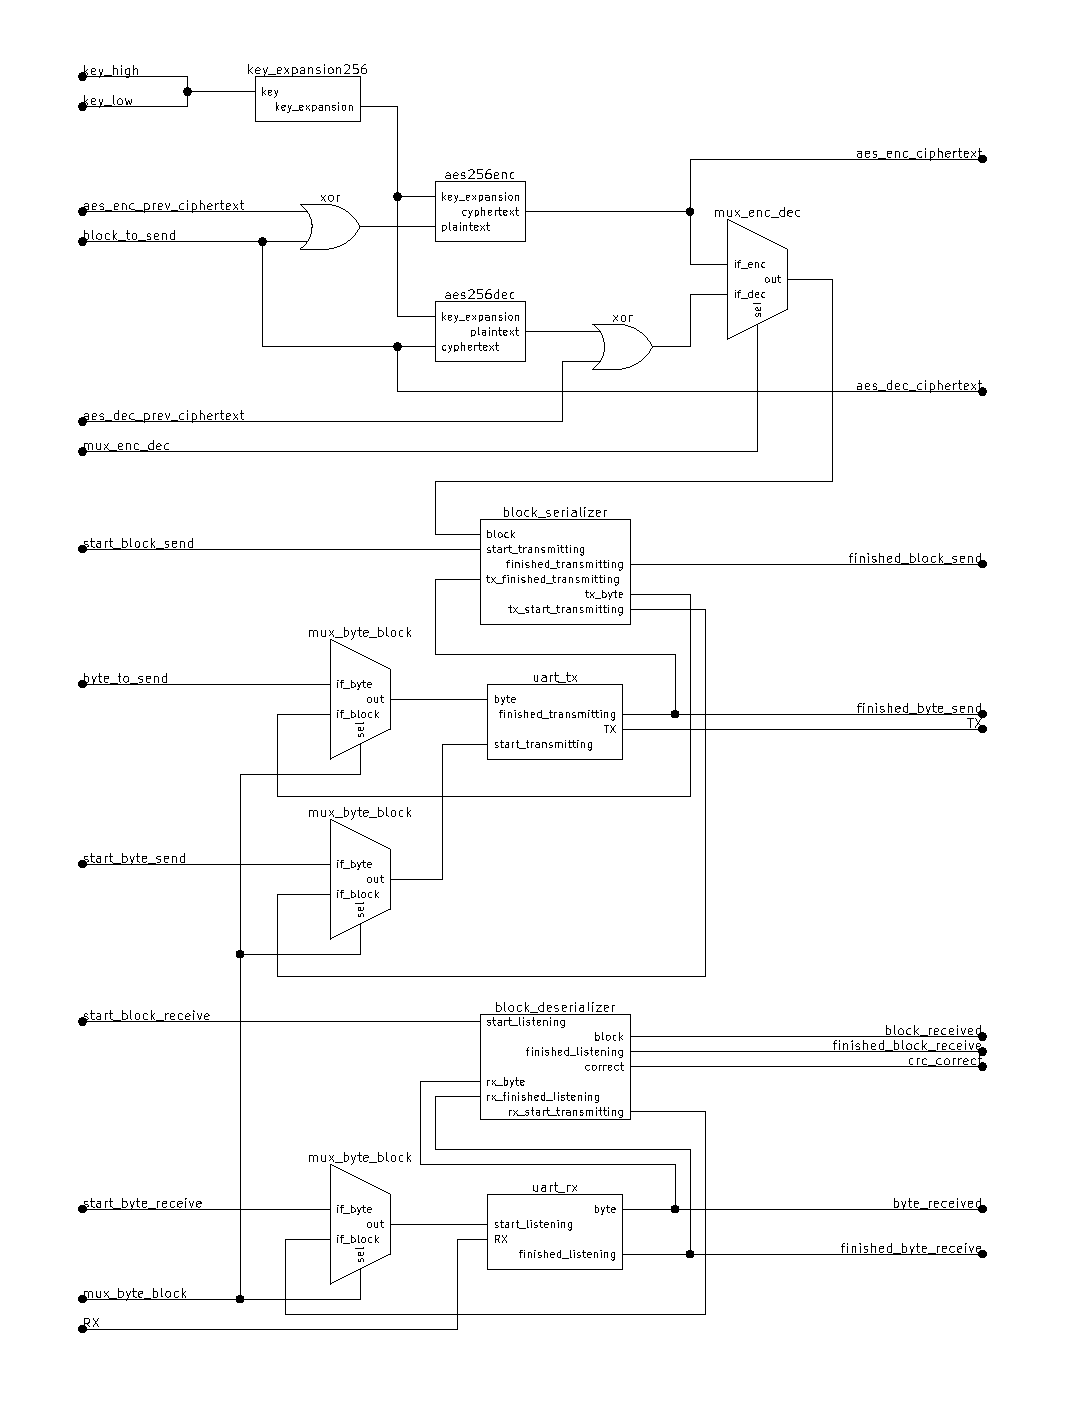
\includegraphics{pictures/communicator.pdf}
\caption{Schemat modułu \textit{communicator}}
\label{fig:communicator-schemat}
\end{figure}

%%%%%%%%%%%%%%%%%%%%%%%%%%%%%%%%%%%%%%%%%%%%%%%%%%%%%%%%%%%%%%%%%%%%%%%%%%%%%%%%%%%%%%%%%%%%%%%%%%%%%%%%
%%%%%%%%%%%%%%%%%%%%%%%%%%%%%%%%%%%%%%%%%%%%%%%%%%%%%%%%%%%%%%%%%%%%%%%%%%%%%%%%%%%%%%%%%%%%%%%%%%%%%%%%
%%%%%%%%%%%%%%%%%%%%%%%%%%%%%%%%%%%%%%%%%%%%%%%%%%%%%%%%%%%%%%%%%%%%%%%%%%%%%%%%%%%%%%%%%%%%%%%%%%%%%%%%


\newpage
\subsection{Skrypt klienta}
Skrypt klienta jest implementacją algorytmu komunikacji z serwerem szyfrującym (płytką Terasic DE1-SOC) przedstawionego w sekcji \ref{sec:przebieg-komunikacji}. Program przyjmuje od użytkownika tryb działania (szyfrowanie lub deszyfrowanie), klucz szyfrowania, wektor inicjalizacji oraz nazwy plików wejściowego i wyjściowego. Program odczytuje z dysku dane wejściowe, wysyła je do serwera oraz odbiera dane przetworzone i zapisuje je do pliku wynikowego. Jest napisany w języku python, oraz korzysta z bibliotek:
\begin{description}[noitemsep]
\item[serial] -- komunikacja przez port szeregowy UART
\item[threading] -- wielowątkowość związana z jednoczesnym wysyłaniem i odbieraniem bloków
\item[crcmod] -- obliczanie sumy kontrolnej crc16
\item[struct] -- konwersja liczby crc16 do tablicy bajtów możliwej do przesłania biblioteką serial
\item[argparse] -- parsowanie argumentów programu
\item[re] -- obsługa wyrażeń regularnych
\end{description}

\subsubsection{Padding}
Algorytm AES działa na blokach o wielkości 128b. W celu przetwarzania danych o wielkości nie będącej wielokrotnością rozmiaru bloku stosowany jest padding. W tym projekcie należy to do zadań klienta. Używany jest padding metodą dopełniania bloków do rozmiarów 128b bajtami o wartości równej brakującej liczbie bajtów. W celu uniknięcia niejednoznaczności przy usuwaniu wypełnienia, do wiadomości o wielkości będącej wielokrotnością 128b dodawany jest cały blok bajtów o wartości 16. W ten sposób ostatni bajt wiadomości zawsze zawiera liczbę bajtów dopełnienia, co pozwala na jednoznaczne usunięcie paddingu. 

Zastosowana metoda jest jedną ze standardowych praktyk. Została wybrana ze względu na fakt, że jest używana przez program \textit{openssl}, z którym produkt końcowy ma być kompatybilny. Jest zaimplementowana w sposób zgodny ze standardem RFC-2315 \cite{padding-rfc}.


\section{Pomiary wydajności modułu szyfrującego}
Ze względu na zastosowanie protokołu UART do komunikacji wydajność produktu ograniczona jest prędkością transmisji. Moduł szyfrujący AES może jednak działać z szybszą prędkością. W celu zmierzenia wydajności szyfrowania przeprowadzono test wydajnościowy.

\subsection{Metodyka testów}
W celu ustalenia wydajności modułu szyfrującego utworzono nowy projekt. Zaimplementowano układ taktowany zegarem, który na każdym rosnącym zboczu podawał na wejście modułu szyfrującego blok losowych danych oraz porównywał wyjście tego modułu (poprzedni blok w zaszyfrowanej formie) z oczekiwaną wartością. Jeśli przez długi okres czasu (ok. 1 godziny) wszystkie wyniki były poprawne to uznawano, że moduł jest zdolny szyfrować bloki z aktualną częstotliwością zegara.

Do testów użyto 16 różnych par losowych danych wejściowych i ich oczekiwanej postaci zaszyfrowanej. Aby zagwarantować, że kompilator nie zoptymalizuje projektu poprzez uproszczenie modułu szyfrującego lub przeprowadzenie częściowych obliczeń w czasie kompilacji, dane zostały umieszczone w pamięci ROM w układzie FPGA (ang. \textit{on-chip memory}). W czasie działania układu kolejne bloki i wartości oczekiwane są pobierane z pamięci. Użyta została pamięć M10K, która jest w stanie działać z częstotliwością 315MHz (\cite[rozdz. 2]{altera-vol1}). Jest to wartość znacznie większa niż zmierzona maksymalna częstotliwość pracy modułu szyfrującego, więc pamięć nie stanowi wąskiego gardła systemu pomiarowego.

Przyjęto założenie, że klucz w trakcie szyfrowania jest stały -- wszystkie bloki szyfrowane są jednym kluczem, a przy jego zmianie można poświęcić kilka cykli zegara na ustabilizowanie się układu przed przystąpieniem do szyfrowania. Użyty został losowo wygenerowany klucz, który w celu uniknięcia optymalizacji kompilatora również został umieszczony w pamięci i jest wczytywany przez układ przy starcie.

Poprawność szyfrowanych bloków sprawdzana jest przez porównanie wyników z wartościami oczekiwanymi. W przypadku wystąpienia pierwszego błędu zapalana jest dioda LED na płytce Terasic DE1-SOC, co oznacza, że układ nie działa stabilnie przy aktualnej częstotliwości zegara. Zegar o żądanej częstotliwości generowany jest przez układ PLL.

\subsection{Wyniki testów}
Analiza opóźnień przeprowadzona przez narzędzie \textit{TimeQuest Timing Analyzer} będące częścią środowiska Quartus wykazała, że dla najgorszego modelu (\textit{Slow 1100mV 85C Model}\footnote{Slow/Fast -- jakość egzemplarza układu, 1100mV -- napięcie zasilające, 0C/85C -- temperatura działania}) układ może działać poprawnie z częstotliwością 16,13MHz. Przeprowadzone testy na rzeczywistym urządzeniu (układzie FPGA na płytce Terasic DE1-SoC) pokazały, że moduł szyfrujący działa stabilnie przy częstotliwości 20MHz. Dla takiej częstotliwości narzędzie \textit{TimeQuest Timing Analyzer} informuje, że dla najgorszych modeli (\textit{Slow 1100mV 85C Model} oraz \textit{Slow 1100mV 0C Model}) naruszony jest czas ustalania (ang. \textit{setup time}), ale dla modeli szybkich (\textit{Fast 1100mV 85C Model} oraz \textit{Fast 1100mV 0C Model}) analiza czasowa jest bez zastrzeżeń.

Działanie modułu z częstotliwością 20MHz pozwala na zaszyfrowanie z prędkością
\begin{equation*}
20MHz * 128b = 2560b/s = \textbf{320MB/s}
\end{equation*}

\subsection{Interpretacja wyników}
Dla porównania przeprowadzono testy wydajności szyfrowania na komputerze PC wyposażonym w procesor Intel i7 6700K taktowany zegarem 4GHz. Użyto benchmarku w programie VeraCrypt, który dał następujące wyniki:
\begin{description}
\item[243MB/s] Przy wyłączonej akceleracji sprzętowej (szyfrowanie bez użycia instrukcji AES-NI \cite{aes-processors}) przy użyciu jednego wątku
\item[1,1GB/s] Przy włączonej akceleracji sprzętowej (szyfrowanie z użyciem instrukcji AES-NI \cite{aes-processors}) przy użyciu jednego wątku
\end{description}

Zaimplementowany w układzie FPGA moduł szyfrujący jest więc o 30\% szybszy od procesora Intel i7 najnowszej generacji działającego bez użycia instrukcji AES-NI, oraz o 70\% wolniejszy od tego samego procesora wykorzystującego instrukcje AES-NI.

Projekt modułu szyfrującego można jednak optymalizować, np. poprzez zastosowanie przetwarzania potokowego (ang. \textit{pipelining}). Przy podziale modułu na 14  części, po jednej dla każdej rundy szyfrowania, moduł mógłby szyfrować z prędkością nawet czterokrotnie szybszą od współczesnego procesora Intel wykorzystującego sprzętową akcelerację szyfrowania (przy założeniu, że narzut związany z podziałem modułu byłby mały). Badanie wpływu pipeliningu na wydajność modułu szyfrującego nie zostało przeprowadzone -- może być przedmiotem dodatkowych badań.
\section{Możliwości rozwoju}
Otrzymany produkt końcowy może stanowić bazę dla optymalizacji i ulepszeń. W obecnej wersji, ze względu na ograniczenia transmisji UART możliwe jest przesyłanie danych z prędkością jedynie 1MB/90sek. Najważniejszym z proponowanych usprawnień jest zastąpienie tego protokołu komunikacji bardziej wydajnym. Można również rozważyć optymalizacje związane z implementacją logiki szyfrującej w bardziej wydajny sposób, lub integrację układów szyfrujących z procesorami CPU lub innymi układami wykorzystywanymi np. w IoT.

\subsection{Prędkość transmisji}
Zastosowanie w projekcie protokołu UART do komunikacji ma negatywny wpływ na wydajność produktu. Zastosowane parametry transmisji (115200 baud, 1 bit stopu, brak bitu parzystości) oraz narzut na komunikację związany z koniecznością kontroli poprawności przesyłanych danych powoduje, że maksymalna prędkość transmisji danych wynosi jedynie 1MB/90s. Jest to ograniczenie wynikające wyłącznie z wybranego sposobu komunikacji. Wydajność modułu szyfrującego i deszyfrującego jest o wiele wyższa. Produkt można usprawnić stosując inny protokół komunikacji, który pozwoliłby na osiąganie wyższych prędkości transmisji danych.

Istnieją układy FPGA, które są zintegrowane z procesorem ARM (np. układ Altera Cyclone V na płytce Terasic DE1-SOC, która była użyta w tym projekcie). Posiadają one szybki interfejs między HPS a programowalną częścią układu. Przykładem zastosowania takiego połączenia jest uruchomienie systemu operacyjnego na procesorze ARM oraz zaprogramowanie i wykorzystanie części FPGA jako sprzętowego układu szyfrującego. Wydajność takiego rozwiązania niewątpliwie nie była by tak drastycznie ograniczona przez prędkość transmisji.

\subsection{Implementacja modułu szyfrującego}
W tym projekcie moduł szyfrujący jest asynchroniczny -- nie jest taktowany zegarem. Wydajność takiego rozwiązania można poprawić stosując potokowość (ang. \textit{pipelining}) -- zaprojektować układ synchroniczny, który w każdym takcie zegara wykonuje pewien fragment procesu szyfrowania, dla wielu bloków jednocześnie. Przykładem podziału procesu szyfrowania na etapy może być podział na rundy -- moduł szyfruje jednocześnie wiele bloków, każdy w innej rundzie.

Można również rozważyć zaprojektowanie modułu, który byłby mniej skomplikowany i zużywał mniej programowalnych jednostek układu FPGA. Większość procesu szyfrowania AES to powtarzanie tej samej operacji (rundy). Można zaprojektować synchroniczny układ szyfrujący tak, aby szyfrowanie trwało wiele taktów zegara, oraz w każdym takcie stan był modyfikowany przez ten sam układ logiczny. Zmniejszyłoby to zapotrzebowanie na zasoby, ale mogłoby to pogorszyć szybkość szyfrowania.

\subsection{Poprawa obsługi błędów}
Obecnie moja implementacja komunikacji obsługuje jedynie błędy związane z przekłamaniem bitów danych podczas transmisji UART. Nie są obsługiwane błędy związane ze złym formatem ramki UART (ang. \textit{framing error}). Wystąpienie takich błędów może spowodować zawieszenie układu. Zaimplementowany został przycisk reset, który przywraca układ do stanu początkowego, który jest sposobem na wyprowadzenie układu z zawieszenia. Takie rozwiązanie można poprawić implementując obsługę błędów formatu ramki, np. timeout. Wyeliminowałoby by to konieczność ręcznego resetowania układu w przypadku wystąpienia błędu.

Błędy związane ze złym formatem ramki mogą wystąpić, jednak podczas testowania nie zostały zaobserwowane.

\subsection{Integracja z procesorem}
Obecnie popularne procesory są wyposażone w zestaw instrukcji AES-NI przeznaczonych do szyfrowania AES \cite{aes-processors}. Przykładem takich jednostek są procesory Intel (począwszy od architektury Westmere -- 2010r.) oraz AMD (począwszy od architektury Bulldozer -- 2011r.) Propozycją polepszenia wydajności lub zmniejszenia poboru prądu podczas szyfrowania AES jest wyposażenie procesorów w zintegrowany sprzętowy układ szyfrujący, podobnie jak to ma miejsce ze zintegrowanymi GPU. Takie rozwiązanie wymagałoby jednak sprawdzenia, czy jest opłacalne. Możliwe jest, że zyski wynikające z takiego rozwiązania nie były by na tyle duże, aby uzasadnić koszty związane z zastosowaniem takiego rozwiązania.

\subsection{Zastosowanie w IoT}
Obecnie jedną z szybko rozwijających się koncepcji jest Internet of Things. Sprzętowe szyfrowanie AES mogło by znaleźć w niej zastosowanie. Można by zaprojektować układ szyfrujący optymalizujący zużycie energii. Pozwoliłoby to na zastosowanie go w urządzeniach, które zasilane są przy pomocy baterii i od których oczekuje się, że będą działać przez długi okres czasu bez konieczności jej wymiany. Taki dedykowany układ  szyfrujący, w porównaniu do szyfrowania przy pomocy procesorów ogólnego przeznaczenia, mógłby pozwolić na dłuższy czas pracy urządzeń IoT.
	
\listoffigures
\lstlistoflistings

\bibliography{../common/bibliografia}
\end{document}
